\documentclass[binding=0.6cm, LaM]{sapthesis}
\usepackage{microtype}
\usepackage[english]{babel}
\usepackage[utf8]{inputenx}
\usepackage{hyperref}
\usepackage{wasysym}
\usepackage{siunitx}
\usepackage{biblatex}
\usepackage{titlesec}
\usepackage{float}
\usepackage{xcolor}
\newcommand{\fpg}[1]{\textcolor{red}{#1} }
\addbibresource{sample.bib}
\hypersetup{pdftitle={My thesis},pdfauthor={Giada Caneva Santoro}}
\usepackage{amsmath, amssymb}
\title{Coherent and Coincident Analyses of LIGO-Virgo Data from the Third Observing Run}
\author{Giada Caneva Santoro}
\IDnumber{1490713}
\course{Facolt\`a di Scienze Matematiche Fisiche e Naturali}
\courseorganizer{Corso di Laurea Magistrale in Fisica}
\AcademicYear{2018/2019}
\copyyear{2020}
\advisor{Dr. Francesco Pannarale Greco}
\authoremail{giada.greenday92@gmail.com}
\DeclareUnicodeCharacter{2212}{-}
\begin{document}

\frontmatter
\maketitle
\dedication{Fortsett å gå.}


\tableofcontents

\mainmatter 

\chapter{Introduction}
\fpg{Non ancora letto.}%
	More than 100 years ago, Albert Einstein predicted the existence of gravitational waves,
	GWs, on the basis of his theory of general relativity.  
	Einstein predicted that the motion of two bodies, such as planets or stars—orbit each other,
	could cause distortions of spacetime, GWs \cite{1,2}, 
	These ripples in the fabric of spacetime would spread out like the ripples in a pond when a stone is tossed in,
	although their amplitude would be so small that it would be nearly impossible to detect by any technology foreseen at that time.
	It was also predicted that objects moving in an orbit would lose energy for this reason 
	(a consequence of the law of conservation of energy), as some energy would be given off as GWs, 
	although this would be insignificantly small in all but the most extreme cases. 
	GWs squeeze and stretch anything in their path as they pass by. \\
	The most powerful GWs are created when objects move at very high speeds. 
	Examples of such things are orbiting pairs of black holes (BHs) and neutron stars (NS), 
	or massive stars blowing up at the ends of their lives.
	There are four categories of GWs based on what generates them: 
	continuous, compact binary inspiral, stochastic, and burst. 	
	Each category of objects generates a unique or characteristic set of signal 
	that LIGO-Virgo's interferometers can sense, and that researchers can look for in LIGO-Virgo’s data. \\ 
        The interferometers are designed to detect a specified range of frequencies of GWs,
        which means that they cannot detect objects orbiting at rates that fall outside of this range of frequencies 
        (either too low or too high). 
	During the final moments of the merger of two compact objects such as NSs 
	or BHs the emission of GWs is at its peak. The binary loses energy, 
	largely through GWs, and as a result, the two compact objects spiral in towards each other, 
	reaching extreme velocities at the very end of this process. 
	In the final fraction of a second of their merger a significant amount of their mass is converted into gravitational energy, 
	and travel outward as GWs, that potentially fall within the detector’s sensitive range. \\
	However, the time they spend orbiting in that range of frequencies is typically very brief.
        The masses of the objects involved dictate how long they emit detectable GWs. 
        Heavy objects, like BHs, move through their final inspiral phase much more rapidly than 'lighter' objects, 
        like NSs. This means that BH  merger signals are much shorter than NS merger signals.
        For example, the first detection of a GW signal, GW150914, coming from the a pair of merging BHs, 
	produced a signal just two-tenths of a second long \cite{14}. 
        In contrast, the first NS merger LIGO detected in August 2017 generated a signal over 100 seconds long \cite{15}. \\
	This first observation was a a remarkable accomplishment: it demonstrated both the existence of binary stellar-mass BH systems, 
	and the fact that such mergers could occur within the current age of the universe.  
	It also confirmed the last remaining unproven prediction of general relativity and validated 
	its predictions of spacetime distortion in the context of large scale cosmic events. 
	Prior to this first detection, GWs had only been inferred indirectly,
        via their effect on the timing of pulsars in binary star systems.
	This event  marked the beginning of a new era of GW astronomy, 
	which would enable observations of violent astrophysical events that were not previously possible, 
	and potentially allow the direct observation of the birth of the universe.


%----------------------------------------------------------------------------------------------------------------------------------------------------------------------------------------------------------
\chapter{Gravitational-Wave Detection Principles}
\fpg{Una lettura.}%
	The aim of this thesis is to expose the methodologies involved 
	in compact binary coalescence through gravitational wave observation. 
	Before giving into this topic, it is useful to shortly discuss gravitational waves, 
	the theory behind them and the instrumental apparatus that is being used to detect them. 
	In this chapter we give a broad outline of these subjects, 
	without going too deep into details. \\
	We begin by introducing the basics of gravitational wave theory in section 2.1. 
	In section 2.2 we discuss gravitational wave interferometric detectors. 
	In section 2.3 we briefly describe the noise sources that affect the detection. 
	Finally. in section 2.4, we describe the astrophysical sources of gravitational radiation.

\section{Gravitational waves in linearized gravity}

	In 1915, Albert Einstein presented his general theory of relativity
	The classical Newtonian notion of gravity, which stated that gravity arises from an 
	action at a distance, was replaced by a geometric interpretation of the Universe, 
	the spacetime continuum: this may be regarded as a fabric and that can be curved 
	by mass \cite{1}. 
	The motion of masses on this curved spacetime fabric will then be perceived as gravity. 
	In general relativity, spacetime is regarded as a four-dimensional manifold 
	with a Lorentzian metric, and gravity is a manifestation of the manifold’s curvature. \\
	The space-time curvature is associated with the stress-energy tensor 
	of matter fields through the Einstein field equation:
		\begin{equation}
		G_{\mu\nu} \equiv R_{\mu\nu}  - {1 \over 2}g_{\mu\nu}R = {8\pi G_{N} \over {c^4}}T_{\mu\nu} 
		\end{equation}
	where $G_{\mu\nu} $ is the Einstein tensor, $T_{\mu\nu} $ is the stress-energy 
	tensor of matter-fields, $ G_{N}$ is Newton’s gravitational constant and $c$ the speed of light. \\
	In 1916 Einstein found the weak-field solutions to general relativity had wave-like solutions, GWs.
	GWs are ripples in the fabric of spacetime, 
	which periodically lengthen and shorten space, and speed up and slow down time \cite{2}.
 	To study the properties of GWs, it is instructive to first study them 
	in situations where the gravitational fields are weak.
	In the so-called weak-field approximation, one can view the metric as the Minkowski metric 
	with a small perturbation: the Einstein equations can be expanded around the flat-space metric, of special relativity. \\
	Letting $ x_\mu = (t, x, y, z)$ denote the time and space coordinates, 
	we can write the proper distance between events $x_{\mu}$ and $x_{\mu} + dx_{\mu}$ as
		\[
		ds^2 = g_{\mu\nu}dx^{\mu}dx^{\nu} \approx (\eta_{\mu\nu} + h_{\mu\nu})dx_{\mu}dx_{\nu}. \hspace*{2cm}\|h_{\mu\nu}\|\ll 1
		\]
	Here $\eta_{\mu\nu} = diag(-1,1,1,1)$ is the usual Minkowski metric and the metric perturbation  $h_{\mu\nu}$        
	represents the linearised gravitational field, it encapsulates GWs, 
	but contains additional, non-radiative degrees of freedom as well. $\|h_{\mu\nu}\|$ means
	“the magnitude of a typical non-zero component of $h_{\mu\nu}$”. 
	The condition $\|h_{\mu\nu}\|\ll 1$ requires both the gravitational field to be weak, 
	and constrains the coordinate system to be approximately Cartesian.  \\
	In linearized gravity, the smallness of the perturbation means that only terms which are linear in $h_{\mu\nu}$ are considered;
	higher order terms are discarded. As a consequence, indices are raised and lowered using the flat metric. 
	The metric perturbation $h_{\mu\nu}$ transforms as a tensor under Lorentz transformations, 
	but not under general coordinate transformations: since the numerical values of the components
	of a tensor depend on the reference frame, there exists a reference frame in which 
	the linearisation of the gravitational field holds on a sufficiently large region of the spacetime. \\
	The Einstein field equations are covariant under general coordinate transformations
		\begin{equation}
		x^{\mu} \rightarrow x^{\mu ‘}(x)
		\end{equation}
	So that the metric transforms as
		\begin{equation}
		g_{\mu\nu} \rightarrow g_{\mu' \nu'} = x^{\rho},_{\mu'}x^{\sigma},_{\nu'}g_{\rho \sigma}
		\end{equation}
	This means that one is free to choose a convenient coordinate system without 
	altering the physical predictions of the field equations \cite{16}. \\
	Choosing a reference frame breaks the invariance of general relativity under 
	coordiante trasformations but it also erases spurious degrees of freedom. 
	After choosing a frame where the field is linearised, 
	a residual gauge symmetry remains. \\
	Under infinitesimal coordinate transformations
                 \[
			x_{\mu} \rightarrow x_{\mu} + \xi_{\mu}
                \]
	using the transformation law of the metric, to lowest order $h_{\mu\nu}$ transforms as	
		\[
			h_{\mu\nu} \rightarrow h_{\mu\nu} - \partial_{\mu}\xi_{\nu} - \partial_{\nu}\xi_{\mu}
		\]
	Rather than working with the metric perturbation, changing notation and using the trace-reversed perturbation 
	makes the computation more compact and cleaner. We define
		\begin{equation}
			{\bar h}_{\mu\nu} = h_{\mu\nu} - {1 \over {2}}\eta_{\mu\nu}h  
		\end{equation}
	the trace
		\begin{equation}
			h = \eta^{\mu\nu}h_{\mu\nu}
		\end{equation}
	and express the trace-reversed field:
		\begin{equation}
			h_{\mu\nu} = {\bar h}_{\mu\nu} + {1 \over {2}}\eta_{\mu\nu}{\bar h}
		\end{equation}
	The Rienmann tensor constructed in the linearised theory is given by
		\begin{align}
			R^{\mu}_{\nu\rho\sigma} &= \partial_{\rho} \Gamma^{\mu}_{\nu\sigma} - \partial_{\sigma}\Gamma^{\mu}_{\nu\rho}  \\
				       &= {1 \over 2} (\partial_{\rho}\partial_{\nu}h^{\mu}_{\nu\rho} + \partial_{\sigma}\partial^{\mu}h^{\nu\rho} - \partial_{\rho}\partial^{\mu}h^{\nu\sigma} - \partial_{\					     \sigma}\partial_{\nu}h^{\mu}_{\rho})
		\end{align}
	From this, the Ricci tensor takes the form
		\begin{equation}
			R_{\mu\nu} = R^{\rho}_{\mu\rho\nu} = {1 \over 2}(\partial_{\rho}\partial_{\nu}h^{\rho}_{\mu} + \partial^{\rho}\partial_{\mu}h_{\nu\rho} - \square h_{\mu\nu} - \partial_{\mu}\partial_{\nu}h)
		\end{equation}
	The curvature scalar is obtained contracting once more:
		\begin{equation}
			R = R^{\mu}_{\mu} = (\partial_{\rho}\partial^{\mu}h^{\rho}_{\mu} - \square h)
		\end{equation}
	Finally, the Einstein tensor can be expressed as
		\begin{equation}
			G_{\mu\nu} = {1 \over 2}(\partial_{\rho}\partial_{\nu}h^{\rho}_{\mu} + \partial^{\rho}\partial_{\mu}h_{\nu\rho} - \square h_{\mu\nu} - \partial_{\mu}\partial_{\nu}h - \eta_{\mu\nu}\partial_{\rho}\partial^{\sigma}h^{\rho}_{\sigma} + \eta_{\mu\nu}\square h)
		\end{equation}
	Substituting the metric perturbation $h_{\mu\nu}$  with the $trace-reversed$ perturbation ${\bar h}_{\mu\nu}$ and expanding, 
	the linerised Einstein equations take the compact form:
		\begin{equation}
			\square {\bar h}_{\mu\nu} + \eta_{\mu\nu}{\partial}^{\rho}{\partial}^{\sigma}{\bar h}_{\rho\sigma} - {\partial}^{\rho}{\partial}^{\nu}{\bar h}_{\mu\rho} - {\partial}^{\rho}{\partial}^{\mu}{\bar h}_{\nu\rho} = - {{16\pi G_{N}} \over {c^4}}T_{\mu\nu}.
		\end{equation}
	The linearised equations of motion are gauge-invariant, and the gauge freedom can
 	be used to simplify the form of the field equations \cite{17}.
 	In the Lorentz family of gauges, choosing the harmonic gauge $ \partial_{\mu}h_{\mu\nu} = 0 $ 
	reduces the Einstein equations to a simple wave equation that relates the trace-reversed field
 	to the stress energy tensor:
		\begin{equation}
			\label{reduceinstein}
			\square {\bar h}_{\mu\nu} =({\partial^2 \over {\partial t^2} } - {\partial^2 \over {\partial x^2}}  - {\partial^2 \over {\partial y^2}}  -  {\partial^2 \over {\partial z^2}}) {\bar h}_{\mu\nu} = -{{16\pi G_{N}} \over {c^4}}T_{\mu\nu}. 
		\end{equation}
	By imposing the harmonic gauge one has chosen the coordinates in such a way that for a single plane wave 
	(or a superposition of plane waves with their wave vectors pointing in the same direction),
	the GW polarisations are perpendicular to the direction of propagation.
	The harmonic gauge gives four conditions, that reduce the ten indipendent components of  
	$h_{\mu\nu}$ to six indipendent components, so it does not fix the gauge completely,
	leaving four additional components free to be gauge-fixed.
	If the metric perturbation is not in the harmonic gauge, by making an infinitesimal coordinate transformation
		\begin{equation}
			{\bar h}_{\mu\nu} \rightarrow {\bar h}_{\mu’\nu’}  = {\bar h}_{\mu\nu}  - \xi_{\mu,\nu} -\xi_{\nu,\mu} + \eta_{\mu\nu}\xi^{\rho}_{,\rho}
		\end{equation}
	and applying the harmonic gauge condition
		\begin{equation}
			{\bar h}_{\mu’\nu’,} ^{\nu’} = {\bar h}_{\mu\nu,} ^{\nu} - \xi_{\mu,\nu}^{\nu}
		\end{equation}
	Therefore any metric perturbation can be put into an harmonic gauge by making an infinitesimal 
	coordinate transformation that satisfies
		\begin{equation}
			{\bar h}_{\mu\nu,} ^{\nu} = \xi_{\mu,\nu}^{\nu}
		\end{equation}
	This is a wave equation that always admits a solution, thus one can always achieve the harmonic gauge. 
	Outside the source where $T_{\mu\nu} = 0$ Eq.$\ref{reduceinstein}$ reads 
		\begin{equation}
			\square {\bar h}_{\mu\nu} = 0
		\end{equation}
	In asymptotically flat ($h_{\mu\nu} \rightarrow 0$ as $r \rightarrow 0$) vacuum spacetimes, 
	the metric perturbation can be greatly simplified using
	the residual gauge freedom within the harmonic gauge class \cite{4}. 
	The transverse-traceless $TT$-gauge can be obtained by choosing the components of the metric tensor $h_{\mu\nu}$
	so that only the ones on the plane orthogonal to the direction of propagation (transverse) 
	are different from zero; this results in $h_{\mu\nu}$ being traceless:
		\begin{equation}
			h^{0\mu} = 0 \hspace*{0.5cm}  h^{i}_i = 0  \hspace*{0.5cm}   {\partial}^jh_{ij} = 0
		\end{equation}
	By imposing the harmonic gauge, the ten degrees of freedom of $h_{\mu\nu}$ 
	have reduced to six degrees of freedom, and the residual gauge freedom,
	associated to the four functions $\xi^{\mu}$, has further reduced these to just two degrees of freedom, 
	which correspond to the two possible polarization states of the GW. 
	Equation (2.17) has plane wave solutions $h_{\mu\nu}^{TT}(x)=e_{ij}(k)e^{ikx}$ with 
	$k^{\mu}=(\omega/c,k)$ and $\omega/c=|k|$. The tensor $e_{ij}(k)$ is called the polarization tensor. \\
	In vacuum spacetimes, a plane GW with a given wave-vector $k$ is characterized 
	by two functions $h_+$ and $h_{\times}$, while the remaining components can be set to zero by
	choosing the transverse-traceless gauge. 
	Along the z axis:
		\begin{equation} 
		h_{\mu\nu}^{TT} = 
		\begin{bmatrix}
		0 & 0 & 0 & 0 \\
		0 & h_{+} & h_{\times} & 0 \\
		0 & h_{\times} & -h_{+} & 0 \\
		0 & 0 & 0 & 0 
		\end{bmatrix}\cos{\omega(t-z/c)}
		\end{equation}

\subsubsection{Geodesic equation and geodesic deviation}

	The usual notion of “gravitational force” disappears in general relativity, replaced instead 
	by the idea that freely falling bodies follow geodesics in spacetime.
	Geodesics are the curved-spacetime equivalents of straight lines, which can be found by 
	parallel transporting the tangent vector of a curve \cite{16}. \\
	Given a spacetime metric $g_{\mu\nu}$ and a set of spacetime coordinates $x^{\mu}$, 
	geodesic trajectories are given by the equation:
		\begin{equation}
			{{d^2x^{\mu}}\over{d\tau^2}} + \Gamma_{\nu\rho}^{\mu}(x){{dx^{\nu}}\over{d\tau}}{{dx^{\rho}}\over{d\tau}} = 0 \hspace*{2cm} m \neq 0
		\end{equation}
		\begin{equation}
			{{d^2x^{\mu}}\over{d\lambda^2}} + \Gamma_{\nu\rho}^{\mu}(x){{dx^{\nu}}\over{d\lambda}}{{dx^{\rho}}\over{d\lambda}} = 0 \hspace*{2cm} m = 0
		\end{equation}
	which is the classical equation of motion of a test mass in the curved background described 
	by the metric $g_{\mu\nu}$, in the absence of an external non-gravitational force and where $m$ is the mass
	of the object, $\tau$ represents the proper time given by $d\tau^2 = -ds^2$, 
	and $\lambda$ is some affine parameter along the geodesic. \\
	In a flat spacetime, two straight lines that are initially parallel to each other will remain parallel. \\
	In a curved spacetime, geodesics do not satisfy this property.
	Instead, two nearby geodesics, separeted by $\zeta^{\mu}$, follow the geodesic deviation equation
		\begin{equation}
			{{D^2\zeta^{\mu}}\over{D\tau^2}} = -R^{\mu}_{\nu\rho\sigma}\zeta^{\rho}{{dx^{\nu}}\over{d\tau}}{{dx^{\sigma}}\over{d\tau}}
		\end{equation}
	where $D/D\tau$ is defined as
		\begin{equation}
			{{DV^{\mu}}\over{D\tau}} \equiv {{dV^{\mu}}\over{d\tau}} + \Gamma^{\mu}_{\nu\rho}V^{\nu}{{dx^{\rho}}\over{d\tau}}
		\end{equation}
	and denotes the covariant derivative along a curve parameterised by $\tau$. 
	The geodesics deviation equation describes the change in separation $\zeta^{\mu}$ between two nearby geodesic. \\
	As the Rienmann tensor describes the tidal forces caused by the gravitational field, 
	the geodesic deviation equation shows that tidal forces can be considered as deviations of nearby geodesics \cite{6}.

%----------------------------------------------------------------------------------------------------------------------------------------------------------------------------------------------------------
\section{Gravitational-wave detection with laser interferometers}

	Electromagnetic waves interact strongly with matter, while GWs travel unperturbed through space,
        as they interact only very weakly with matter. This makes them an excellent probe for astrophysical phenomena that are dark
        in the electromagnetic channel, such as the coalescence and merger of BHs, the collapse of a stellar core,
  	the dynamics of the early Universe. \\
	However, it also means that detecting GWs is extremely challenging.
        Electromagnetic radiation typically has a wavelength smaller than the size of the emitting system,
        and so can be used to form an image of the source, while the wavelength of gravitational radiation is typically comparable
        to or larger than the size of the radiating source \cite{18}. 
        Because GWs are generated by the bulk dynamics of the source itself therefore they cannot be used to form an image:
        the radiation simply does not resolve the generating system.
        In most cases, electromagnetic astronomy is based on observers obtain a large amount of information about sources on a small piece
        of the sky while GW astronomy is intrinsically an all-sky approach \cite{4}. \\
	The experimental search for GWs was initiated by Joseph Weber in the early 60  \cite{7}.
	Weber’s first GW detector was a resonant bar detector; 
	the detection’s principle behind these instruments is that 
	they would be set into oscillation at their resonant frequency 
	by passing GWs near that resonant frequency.
	For this purpose, Weber designed and built a big aluminum cylinder as a sort of antenna, 
	hung by a steel wire from a support to isolate vibrations of its environment. 
	The whole instrument was placed inside a vacuum chamber 
	and the cylinder surrounded by a belt of piezoelectric crystal, 
	to sense cylinder vibrations induced by GWs.
	Even though, over the course of the following years, the bar detectors’ sensitivity increased, 
	it did not reach a level where they would be able to detect an extragalactic source. \\
	The first explicit suggestion of a laser interferometer detector 
	was outlined by Gertsenshtein and Pustovoid in 1962 \cite{8}. \\
	From the early 2000s, several kilometer-scale ground-based interferometers 
	operated in the frequency band from 10 Hz to 1 kHz at a sensitivity 
	that all owed the potential for detection from a variety 
	of sources at large extragalactic distances.

\subsection{Description of laser interferometers}

	The optical layout of the detectors consists in perpendicular 
	Fabry–Perot arm cavities of the Michelson, 
	with lasers running along the 4 km arms, as shown in Fig.$\ref{fig:interferometer}$. 
	A beam splitter directs 1064 nm light from a diode-pumped, power amplified, 
	and intensity and frequency stabilized Nd:YAG laser to the Fabry-Perot arms, 
	which are made of an input test mass mirror and an end test mass mirror. 
	The two beams of laser light that return from the two arms are recombined out of phase so that, 
	in principle, no light reaches the so-called 'dark fringe' of the detector. 
	The oscillating quadrupolar strain pattern of a GW, 
	as seen in Fig.$\ref{fig:ring}$, is well matched by a Michelson interferometer,
        which makes a very sensitive comparison of the lengths of its two orthogonal arms.
	Any variation caused by an alteration in the distance between the mirrors, 
	produces a very small shift in phase between the beams and, thus, 
	a variation of the intensity of the light, which is proportional to the wave's amplitude. \cite{10}. \\
	The Fabry-Perot arms are a modification to the Michelson 
	that increases the change in phase measured compared to that for a simple Michelson: 
	because of multiple reflections that occur within each cavity, 
	the tiny distance variation caused by a GW is amplified. 
	All the main interferometer optical components and beam paths are enclosed in the ultra-high vacuum system
        $(10^{−8} - 10^{−9} torr)$ for acoustical isolation and to reduce phase fluctuations from light scattering off residual gas.
        The photodetectors are all located outside the vacuum system, mounted on optical tables.
        The beam tubes are made from stainless steel and are designed to have low-outgassing
        so that the required vacuum can be attained by pumping only from the ends of the tubes \cite{11}. 
        The interferometer optics, including the test masses, are manufactured to have extremely low scatter and low absorption. \\
	The GW detectors offer the possibility of very high sensitivities over a wide range of frequency and
        are particularly suited for the detection of local perturbations in the spacetime metric from astrophysical sources,
        such as binary BH (BBH), or NS coalescences, asymmetric rapidly spinning NSs,
        and supernovae.
 	Gravitational radiation is produced by oscillating multipole moments of the mass distribution of a system.
        Quadrupole radiation is the lowest allowed form, and is thus usually the dominant form.
        In this case, the GW field strength is proportional to the second time derivative of the quadrupole moment of the source,
        and it falls off in amplitude $h$, the direct observable of gravitational radiation, with distance as $1/r$.
        This comparatively slow fall off with distances means that relatively small improvements in the sensitivity
        of GW detectors can have a large impact on their science:
        doubling the sensitivity of a detector doubles the distance to which sources can be detected,
        increasing the volume of the Universe to which sources are measurable by a factor eight. \\
	The frequency band $1Hz \apprle f \apprle 10^4 Hz$ is targeted by
        ground-based laser interferometric detectors has its low end set by the fact that it is extremely difficult
        to prevent mechanical coupling of the detector to ground vibrations at low frequencies,
        and probably impossible to prevent gravitational coupling to ground vibrations, human activity, and atmospheric motions.
    \begin{figure}[H]
                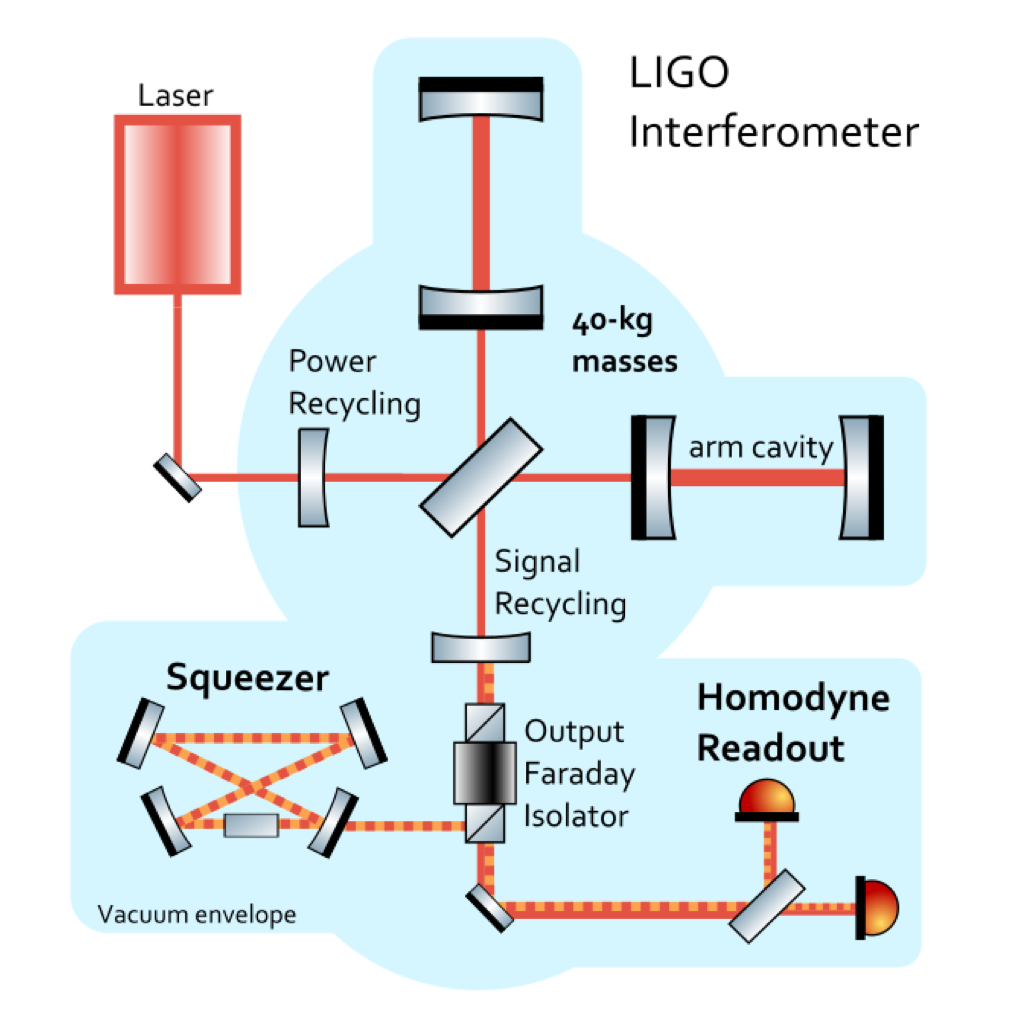
\includegraphics[scale=0.5]{interferometer}
                \centering
                \caption{Simplified schematic of the experimental setup. Several modifications to the Michelson interferometer are shown such as power and signal recycling. The photodetector records the differential lengths of the arms. \cite{9}}
                \label{fig:interferometer}
                \end{figure}

\subsection{Ground-based laser interferometers}

	Detectors have nearly $4\pi$ steradian sensitivity to events over the sky. 
	This means that any source on the sky will be detectable,
        not just sources in specific pointing directions. \\
	A single interferometer is unable to detect GW alone,
	because it us difficult to separate a signal from noise confidently 
	and also provides no directional information about the source.
	A worldwide network of detector is essential to a successful GW detection:
	looking for identical, simultaneous signals from multiple detectors worldwide, 
	rules out noise sources which are local to a given detector. 
	More detectors means a better determination of the direction of GW sources: 
	to reconstruct the location of a transient signal is primarily due to triangulation 
	based on the observed time delays of the signal at several detectors. 
	For more than two sites, requiring a consistency between the observed amplitudes 
	will also serve to restrict the allowed sky positions\cite{12}. \\
	A crucial aspect of the research is to make the instrument sufficiently sensitive:
        at the targeted strain sensitivity of $10^{−21}$ m, the resulting arm length change is only $ 10^{-18}$ m for km-scale instruments, that is
        a thousand times smaller than the diameter of a proton.
        A key feature of the detectors is simply their scale:
        the arms are made as long as practically possible to increase the signal due to a GW strain. \\
	We now briefly list current GW interferometers.

	\begin{itemize}
		\item LIGO. LIGO operates two identical and far apart GW observatories: 
			    LIGO Hanford Observatory (LHO), in Washington, and LIGO Livingston Observatory (LLO), in Louisiana.
			    The sites are separated by roughly 3000 km, 
		   	    and are situated to support coincidence analysis of events.
		       	    LIGO's original instrument engaged in "science observations" from 2002 to 2010. 
			    During this initial phase, the Hanford site operated two collocated interferometers:
			    one detector with 4 km long arms (H1) and another with 2 km long arms (H2). 
			    The Livingston site operated a second 4 km detector (L1). 
			    Each observatory is made up of ultra high vacuum system, 
			    where the interferometer is placed. \\
			    This Advanced LIGO project successfully improved the capabilities of the detectors, 
			    both interferometers were completely overhauled to incorporate much more sophisticated engineering.
		\item Virgo. The Advanced Virgo detector, located in Cascina (near Pisa) in Italy, 
			     is the upgraded version of the Virgo detector. 
			     As LIGO, it is a Michelson interferometer but with 3 km arms.
                 \item GEO600. GEO600 is a 600 m interferometer located near Hannover,
                 	       Germany. It is designed and operated by scientists from the
                               Max Planck Institute for Gravitational Physics and the Leibniz Universität Hannover.
                  \item KAGRA. It is Japan’s first GW detector and also the first GW detector to operate
			       at cryogenic temperatures, improving sensitivity at frequencies around 100 Hz.

\end{itemize}

\section{Interaction of gravitational waves with test masses}
	
	The effects of GWs cannot be seen in isolated bodies. 
	This is a result of the fact that a single test mass, 
	in a frame freely falling with it, will remain at rest.
	At least two test masses are required to measure the effects of GWs. 	
	This is also the case when one wants to measure any curvature of spacetime. \\
        Therefore, to understand how GWs interact with the interferometric detectors,
        it is necessary to use the geodesic equation and the geodesic deviation equation, which are also important tools
        for understanding the physical meaning of a given gauge choice \cite{3}. 
        In fact the physics must be invariant under coordinate trasformations but GWs and the detector description's depend on the chosen reference frame.
        Consider a test mass initially at rest at $\tau = 0$. \\
	The geodesic equation then becomes
                \begin{equation}
                	{{dx^i}\over{d\tau^2}} = -[\Gamma^i_{\nu\rho}{{dx^{\nu}}\over{d\tau}}{{dx^{\rho}}\over{d\tau}}]_{\tau=0} \\ 
                			       = - [ \Gamma^i_{00}({{dx^0}\over{d\tau}})^2]_{\tau=0}
                \end{equation}
        because
                \begin{equation}
                	{{dx^i}\over{d\tau}} = 0 \hspace*{2cm} at \hspace*{0.5cm}\tau = 0
                \end{equation}
        since the mass is initially at rest. Expanding to first order in $h_{\mu\nu}$,
        the Christoffel symbol $\Gamma^i_{00} = 1/2(2\partial_{0}h_{0i} - \partial_i h_{00})$ vanishes in the TT gauge
        because both $h_{00}$ and $h_{0i}$ are set to zero by the gauge condition. \\
        Therefore, if at time $\tau = 0$ $dx^i/d\tau$ is zero, it remains zero at all times,
        because its derivative also vanishes.
        This shows that if two test masses are initially separated by a coordinate separation of $x^i$ in the TT frame,
        and are at rest with respect to each other, they will remain at this separation.
        Overall, it seems that a GW has no influence on the geodesic or on the deviation of geodesics. 
        In other words, in the TT gauge the coordinate location of a slowly moving, free-falling body is unaffected
        by a GW because the coordinates move with the waves \cite{4}. \\
        The TT gauge illustrates that, in general relativity, the physical effects are not expressed by what happens
        to the coordinates since the theory is invariant under coordinate transformations:
        the position of test masses does not change because the gauge freedom allowed to define the coordinates
        in such a way that they do not change \cite{3}.
        Physical effects can instead be found monitoring proper distances, or proper times. 
        GWs cause the proper separation between two freely falling particles to oscillate,
        even if their coordinate separation is constant. Consider two  free-falling particles,
        located at $z = 0$, and separated on the $x$ axis by a coordinate distance $L_c$. \\
        Consider a GW in TT gauge that propagates down the $z$ axis, $h^{TT}_{\mu\nu}(t,z)$.
        The proper distance L between the two particles in the presence of the GW is given by
                \begin{align}
                \label{distance}
                	L & = \int^{L_c}_{0}{dx\sqrt{g_{xx}}} = \int^{L_c}_{0}dx\sqrt{1 + h^{TT}_{xx}(t,z=0)} \\
                	  & \simeq \int^{L_c}_{0}{dx[1 + {1 \over 2}h^{TT}_{xx}(t,z=0)]} \\
                	  &= L_c[1 + {1 \over 2}h^{TT}_{xx}(t,z=0)]
                \end{align}
        Therefore, the proper distance expands and shrinks periodically, with a fractional length change $\delta L/L_c$ given by
                \begin{equation}
                	{{\delta L}\over{L_c}} \simeq {1 \over 2} h_{xx}^{TT}(t,z=0)
                \end{equation}
        Even though this result is calculated in the TT gauge, it is indeed gauge indipendent;
        $h_{xx}^{TT}$ acts as a strain, a fractional length change.
        Because the time that light travels between the two test masses is related to the proper distance,
        which directly relates to the accumulated phase measured by laser interferometric GW observatories,
        GWs leave an imprint on the time it takes for a photon to make a round trip \cite{4}. \\
        Consequently, interferometers can potentially measure these imprints by measuring the length difference between
        their arms. The “extra” phase $\delta \phi$ (if $L \ll \lambda$ so that the metric perturbation
	does not vary during a light travel time) accumulated by a photon that travels
        down and back the arm of a laser interferometer in the presence of a GW is $\delta \phi = 4\pi \delta L \lambda$,
        where $\lambda$ is the photon’s wavelength and $\delta L$ is the distance
        the end mirror moves relative to the beam splitter.

\subsection{Local proper reference frame}

        Since positions in a lab are not marked by test particles,
        the $TT$ frame is not very practical.
        The preferred reference frame is the proper detector frame
        in which the test particle is free to move because of a passing GW.
        The path of a test particle can then be described by Newtonian equations of motion in terms of forces.
        There are terms proportional to the Riemann curvature tensor from the gravitational field of the Earth
        but also terms from static gravitational forces, Coriolis forces, etc \cite{5}.
	GW detectors need to be designed in order to maximise their sensitivity to the part proportional to the Riemann tensor while minimizing their sensitivity to all other terms.
        Consider a detector capable of measuring changes in the proper distance, between two test masses
        and assume the detector has a characteristic size that is much smaller
        than the characteristic wavelength of the GW. \\
        In this case, one can approximate the entire detector to be in a near local Lorentz frame
        (freely falling frame), even in the presence of GWs. This coordinate system is defined by the requirements
                \begin{equation}
                	z^i(\tau) = 0, \hspace*{2cm} g_{ab}(t, 0) = \eta_{ab}, \hspace*{2cm} \Gamma^a_{bc}(t,0) = 0,
                \end{equation}
        which imply that the metric has the form
                \begin{equation}
                	ds^2 \approx -dt^2 + \delta_{ij}dx^i dx^j + O({{x^ix^j}\over{L^2_B}})
                \end{equation}
        where $L^2_B$ denotes the typical variation scale of the metric. \\
        Consider now the proper distance between the two geodesics of the test masses, $\zeta^i$.
        The GWs influence these two test masses via the geodesic deviation equation
                \begin{equation}
                	{{d^2\zeta^{\mu}}\over{d\tau^2}} + 2\Gamma^{\mu}_{\nu\rho}{{dx^{\nu}}\over{d\tau}}{{dx^\rho}\over{d\tau}} + \zeta^{\sigma}\Gamma^{\mu}_{\nu\rho,\sigma}{{dx^{\nu}}\over{d\tau}}{{dx^{\rho}}\over{d\tau}} = 0
                \end{equation}
        Assuming the two test masses are moving non-relativistically, $dx^i/d\tau$ can be neglected compared to $dx^0/d\tau$. \\
        Furthermore, the term proportional to $\Gamma^{\mu}_{\nu\rho}$ is negligible compared to other terms in a near  local-Lorentz frame, LLF. Hence,
                \begin{equation}
                	{{d^2\zeta^{\mu}}\over{d\tau^2}} + \zeta^{\sigma}\Gamma^{i}_{00, \sigma}({{dx^0}\over{d\tau}})^2 = 0
                \end{equation}
        Further simplifying $\zeta^{\sigma}\Gamma^{i}_{00, \sigma} \approx \zeta^{j}\Gamma^{i}_{00, j}$
                \begin{equation}
                	{{d^2\zeta^{\mu}}\over{d\tau^2}} + \zeta^{j}\Gamma^{i}_{00,j}({{dx^0}\over{d\tau}})^2 = 0
                \end{equation}
        But in the LLF, $R^i_{0j0} = \Gamma^i_{00,j} - \Gamma^i_{0j,0} = \Gamma^i_{00,j}$ and therefore
                \begin{equation}
                	{{d^2\zeta^{\mu}}\over{d\tau^2}} + R^i_{0j0} \zeta^j({{dx^0}\over{d\tau}})^2 = 0
                \end{equation}
        Because $dx^0/d\tau \approx 1$, one can approximate $\tau \approx t$:
                \begin{equation}
                	{\ddot \zeta}^j = - R^i_{0j0}\zeta^j
                \end{equation}
        The key quantity entering into the equation, the Rienmann tensor, is gauge invariant in the linearized theory and
        it can be evaluated in any convenient coordinate system. \\
        The expression for the Rienmann tensor in terms of the TT gauge metric perturbation $h_{ij}^{TT}$ is
                \begin{equation}
                	R^i_{0j0} = R_{i0j0} = - {1 \over 2}{\ddot h}_{ij}^{TT}
                \end{equation}
        Substituting into the previous equation, the geodesic deviation equation in the proper detector frame takes the form
                \begin{equation}
                	{\ddot \zeta}^i = {1 \over 2}{\ddot h}_{ij}^{TT}\zeta^j
                \end{equation}
        which can be interpreted as if the influence of a GW in a near LLF resembles a Newtonian force. \\
        Generalizing Eq.$\ref{distance}$, the proper distance may be written as
                \begin{equation}
                	s = \sqrt{L^2 + h_{ij}(t)L_{i}L_{j}}
                \end{equation}
        where $L_i$ denotes the spatial separation between two test masses and $L$ the associated coordinate distance.
        In the given metric for the proper reference frame, the proper distance is just $|L| = \sqrt{L_iL_j}$ up to fractional errors;
        since we are considering detectors such that
        $L \ll \lambda$, these errors are smaller than the fractional distance changes caused by the GW. \\
        Therefore $|L|$ is simply identified as the proper separation. The equation for analyzing an interferometric GW detector is therefore
                \begin{equation}
                	{\ddot L}^i = {1 \over 2}{\ddot h}_{ij}^{TT}L^j
                \end{equation}

\subsection{Ring of test masses}

        Consider a ring of test masses in the $(x, y)$ plane of a proper detector frame, initially at rest, centred at $z = 0$,
        and a GW travelling in the $z$-direction.
        This situation restricts the attention to the $(x,y)$ plane alone, because $h_{ij}^{TT}$ is transverse to the propagation direction,
        so the GW will only have influence in the plane of the test masses:
        the only non zero compontents of the metric perturbation are
                \begin{equation}
                	h_{xx}^{TT} = - h_{yy}^{TT} = h_{+} \hspace*{3cm} h_{xy}^{TT} = h_{yx}^{TT} = h_{\times}
                \end{equation}
        where $h_{+}=h_{+}(t-z)$ and $h_{\times}=h_{\times}(t-z)$ are the two polarization components, which are indipendent and can be considered separately.
        For the plus polarization at $z=0$ and initial conditions $h_{ij}^{TT} = 0$ at $t=0$:
                \begin{equation}
                h_{ab}^{TT} = 
                \begin{bmatrix}
                1  & 0 \\
                0 &  -1 \\
                \end{bmatrix} 
                h_{+}\cos \omega t
                \end{equation}
        If the displacement between geodesics is $\zeta_a (t) = (x_0 + \delta x(t), y_0 + \delta y(t))$, then
                \begin{equation}
                	\delta {\ddot x} = - {{h_{+}} \over 2} (x_0 + \delta x) \omega ^2 \sin \omega t
                \end{equation}
                \begin{equation}
                	\delta {\ddot y} =  {{h_{+}} \over 2} (y_0 + \delta y) \omega ^2 \sin \omega t
                \end{equation}
        Assuming that the perturbations are $O(h)$, and thus small compared to the unperturbed locations, $\delta x$ and $\delta y$ can be neglected.
        The integrations gives the deviations caused by the plus polarisations:
                \begin{equation}
                	\delta x(t) =  {{h_{+}} \over 2} x_0 \sin \omega t
                \end{equation}
                \begin{equation}
                	\delta y(t) = - {{h_{+}} \over 2} y_0  \sin \omega t
                \end{equation}
        Similarly, for the cross polarization at $z=0$ and initial conditions $h_{ii}^{TT} = 0$ at $t= 0$, the situation is described by the equations
                \begin{equation}
                	\delta x(t) =  {{h_{\times}} \over 2} y_0 \sin \omega t
                \end{equation}
                \begin{equation}
                	\delta y(t) =  {{h_{\times}} \over 2} x_0  \sin \omega t
                \end{equation}
        This set of equations describes the changes in the $x$ and $y$ components for a passing GW.
        The plus polarization alternately stretches and compresses the ring of test masses in the x and y directions,
        while the cross polarization exhibits the same behavior rotated by $\ang{45}$ in the $x - y$ plane. This is shown in Figure 2.1.
                \begin{figure}[H]
                \label{ring}
                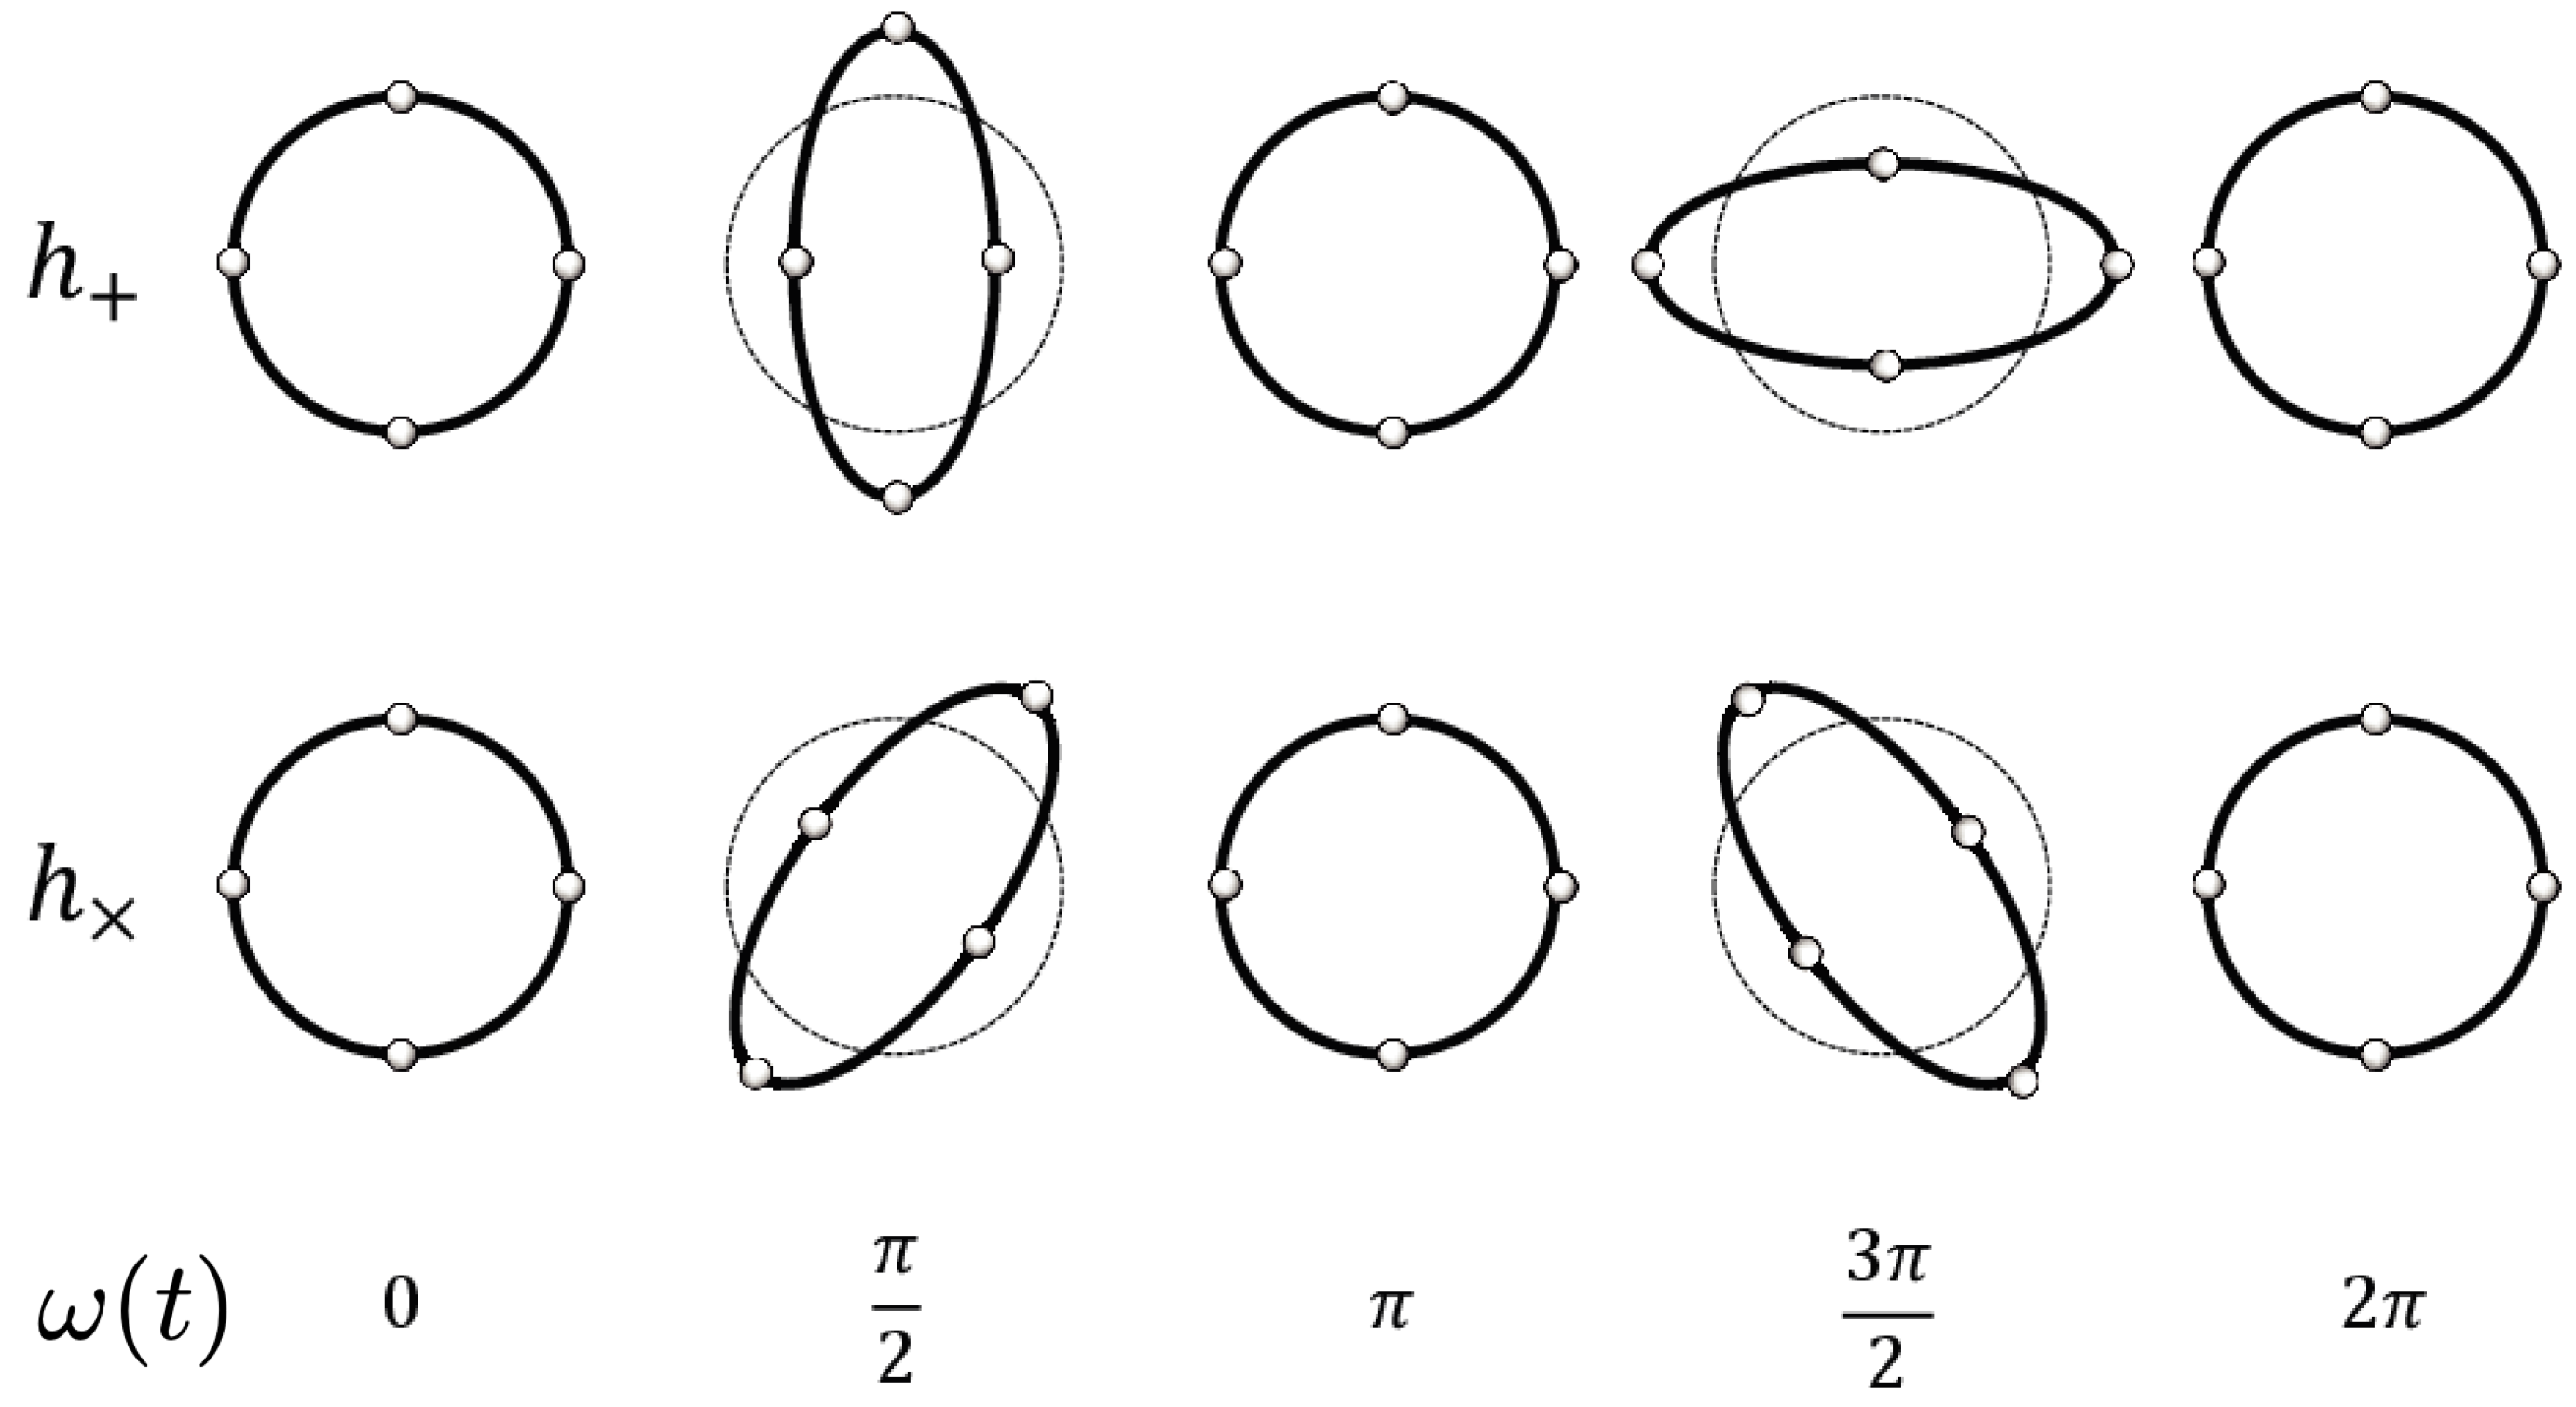
\includegraphics[scale=1]{ring}
                \centering
                \caption{The effects of plus and cross polarization on a ring of test masses. The plus polarization alternately compresses and stretches the x- and y-separations. The cross polarization has the same effect only rotated by  $\ang{45}$.}
                \label{fig:ring}
                \end{figure}

\section{Response of an interferometer to a gravitational wave}

        Interferometers are sensitive to the relative difference between two distances, the so-called strain \cite{6} .
        Suppose we have an interferometer with its arms pointing along the unit vectors $u^i$ and $v^i$. The strain $h(t)$ is given by
                \begin{equation}
                	h(t) = {1 \over 2} (h_{ij}u^iu^j - h_{ij}v^iv^j) = D^{ij}h_{ij}(t)
                \end{equation}
        where $D^{ij}$ is referred to as the detector tensor and is given by
                \begin{equation}
                	D^{ij} = {1\over 2} (u^iu^j -v^iv^j)
                \end{equation}
        As the expression for $h(t)$ is linear in $h_{+}$ and $h_{\times}$, one can also write
                \begin{equation}
		 \label{beampattern}
                	h(t) = F_{+}h_{+} (t) + F_{\times}h_{\times}(t)
                \end{equation}
        where $F_{+,\times}$ are called the beam pattern functions. Suppose we have a detector
        with arms that are perpendicular to each other, one pointing in the x-direction and the other
        in the $y$-direction in a Cartesian coordinate system. This detector frame, denoted by $(x,y,z)$,
        is generally different from the GW coordinate system, denoted by $(x^\prime,y^\prime,z^\prime)$, where the source
        is conveniently described. To account for such a difference, we first note that when the plus
        and cross polarisations are not equal in strength, we can rotate the coordinate system by
        an angle $\psi$ around the $z^\prime$ axis so that the $x^\prime$ and $y^\prime$ axes
        coincide with the mayor and minor axis of the associated ellipse. \\
        In going from the GW frame to the detector frame, we can rotate the GW frame by
        an angle $\theta$ around the $x^\prime$ axis and an angle $\phi$ around the $z^\prime$ axis,
        where the angles $(\theta, \phi)$ denote the direction of propagation of the GW in the detector frame.
        Applying these three rotations, the beam pattern functions for a detector with perpendicular arms are given by
                \begin{align}
                F_{+}^{\ang{90}}& = {1 \over 2} (1 + \cos^2 \theta)\cos 2\phi \cos 2 \psi - \cos \theta \sin2\phi \sin2\psi \\
                F_{\times}^{\ang{90}}& = {1 \over 2} (1 + \cos^2 \theta)\cos 2\phi \sin 2 \psi + \cos \theta \sin2\phi \cos2\psi
                \end{align}

\section{Non-stationary transient noise sources}
	
	The various noises of the detector can be conveniently characterized by a spectral strain
        sensitivity with dimensions of $1/\sqrt{Hz}$, as we explain in this section. 
        The detector output $s(t)$ is composed of instrumental noise $n(t)$ arising from
        naturally occurring random processes and a potential strain signal $h(t)$
                \begin{equation}
                	s(t) = n(t) + h(t)
                \end{equation}
        The detection problem then becomes how to distinguish $h(t)$ from $n(t)$ when $h(t) << n(t)$.
        In a way, $n(t)$ provides a measure of how small an $h(t)$ we can detect.
        Thus we take $n(t)$ as the detector’s noise and have a convenient way to
        compare performances of different detectors.
	The instrument response $s(t)$ can be also expressed as a convolution of the antenna patterns 
	with the two GW polarizations $h_{+}, h_{\times}(t)$:
		\begin{equation}
			s(t) = n(t) +  F_{+}h_{+} (t) + F_{\times}h_{\times}(t)
		\end{equation} 
	The antenna patterns depend on the frequency and sky location of the source; 
	for wavelengths that are large compared to the detector, the antenna patterns are simple quadrupoles \cite{19}.
	The information contained in the time series is usually represented in the Fourier domain 
	as a strain amplitude spectral density, $h(f)$. \\
	This quantity is defined in terms of the power spectral density $S_s(f) = \tilde s^{*}(f) \tilde s(f)$
	of the Fourier transform of the time series:
		\begin{equation}
                	\tilde s(f) = \int^{\infty}_{-\infty} e^{-2 \pi ift} s(t)dt
		\end{equation}
	The strain amplitude spectral density is then defined as $h(f) = \sqrt{S_s(f)}$.
	Noise is categorised as either displacement noise, which directly moves the suspended mirrors
        causing a differential change in the arm cavity lengths, or as sensing noise,
        which appears in the readout signal but is not caused by a GW. \\
        We describe the principal noises that dominate the limits of our sensitivity, (Fig.$\ref{fig:noise2}$).
		\begin{figure}[H]
                        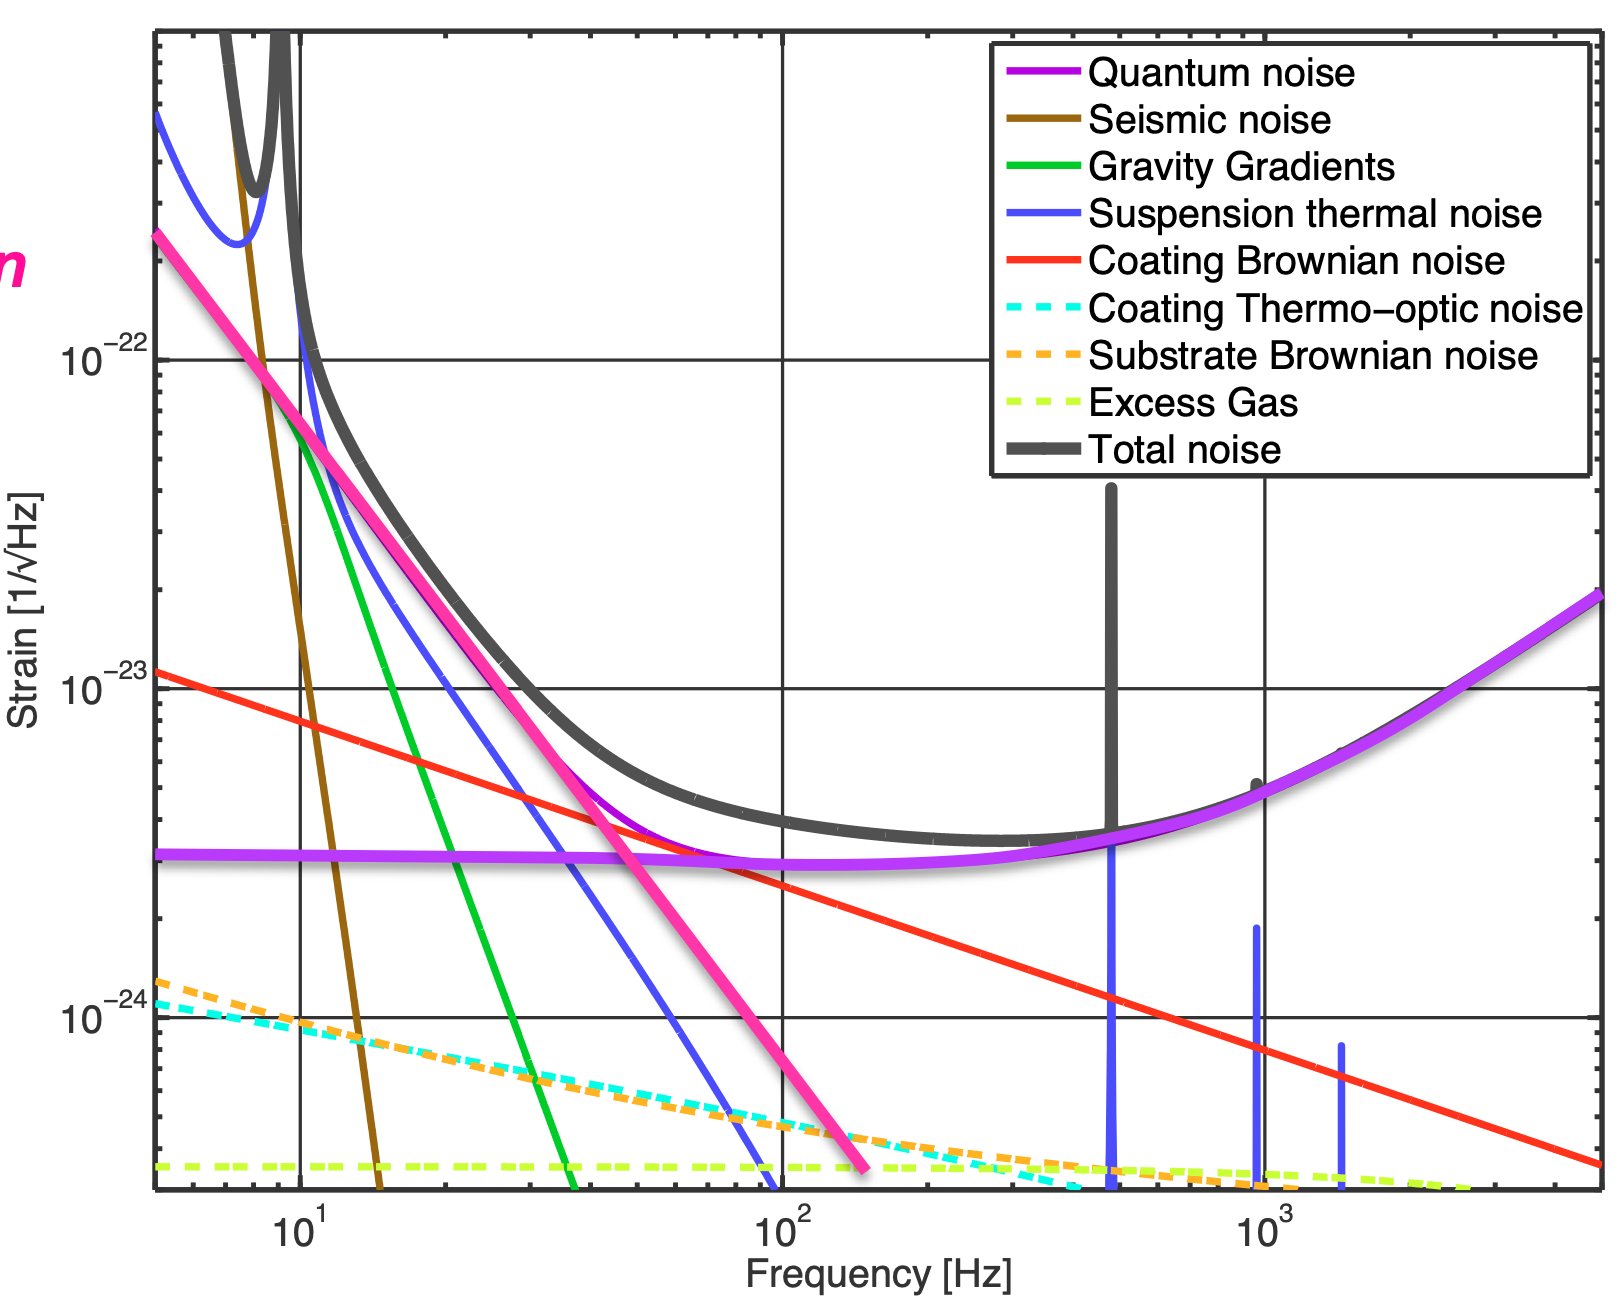
\includegraphics[scale=0.3]{noise2}
                        \centering
                        \caption{The strain equivalent spectral amplitudes $\sqrt{S_n(\omega)}$ of several noises couple to the detector. Most relevant contributions comes from quantum noise and from thermal noise of mirror coating and suspensions. Seismic noise dominates below 10Hz}
                        \label{fig:noise2}
                \end{figure}
        At lower frequencies, up to 10Hz, the main contribution to the global noise
        is due to vibrations of the ground which couple to the mirror motion, (Fig.$\ref{fig:noise2}$ brown line): 
	it shakes the optics and produces strain signals that mask GW signals. 
        This seismic noise is caused by earthquakes, weather and human activity.
        To reduce the potential movements of the optical elements,
        the mirrors are isolated using an advanced suspension system. \\
        At frequencies where the seismic motion has been sufficiently reduced,
        between 10Hz and 500Hz, the random Brownian motion of the molecules on the surface of the mirrors and wires dominates (Fig.$\ref{fig:noise2}$ red line). \\
        The thermal energy of the interferometer’s components induce vibrations both in the suspensions and in the mirrors.
        The nature of GW signal requires the sensitivity of the interferometric detectors
        to be extremely high in broad frequency band.
        Therefore, the power spectrum density of the thermal noise must be considered in the development of the detectors.
        The Fluctuation-dissipation Theorem relates the spectrum of the thermal noise to the amount of dissipation
                \begin{equation}
                	S_{n}(\omega) = - {{4k_bT} \over {\omega}} Im[H(\omega)]
                \end{equation}
        From this equation is possible to state that the energy of fluctuations has a frequency dependent distribution;
        $H(z)$ is the transfer function of the system, it is a mathematical function that models the device’s output, defined as
                \begin{equation}
                	H(x) = {1 \over {iWZ(\omega)}}
                \end{equation}
        In which $Z(\omega)$ is the impedance of the system in the frequency domain that can be computed as the ratio
        between the Fourier components of the generalised force $\tilde F(\omega)$ and the response of the system $\tilde X(\omega)$
                \begin{equation}
                	Z(\omega) = {{\tilde F(\omega)} \over {i\omega \tilde X(\omega)}}
                \end{equation}
        In the case of an harmonic oscillator, the noise spectral density is
                \begin{equation}
                	S_n(\omega) = {{4k_bT} \over {m\omega}} {{{\omega_0}^2 \phi(\omega)} \over {(\omega^2-{\omega_0}^2)^2 + {\omega_0}^4 \phi^2(\omega)}}
		\end{equation} 
	Generally, thermal noise can be reduced decreasing the dissipation with monolithic suspensions and better coatings
        other than lowering the temperature using criogenic payloads as it is done in KAGRA.
        Quantum mechanics limits the precision at which the test mass positions can be determined. \\
        At high frequencies, photon shot noise limits the sensitivity, 
	while at low frequencies it is limited by radiation pressure.
        The photon shot noise is produced by the natural fluctuations in the rate of photons arriving at the photodiode,
        that follow a Poisson process. The noise will decrease with increasing laser power,
        recycling cavity gain, arm cavity gain, and arm length.
        The corresponding noise spectral density is
		\begin{equation}
                	S_n(\omega) = \Bigg({{\lambda_{laser}} \over {4 \pi L}}\Bigg)^2 {{2 \hbar \omega_{laser}} \over {P}}
                \end{equation}
        Radiation pressure noise is associated with the photons from the laser striking the mirror
        and causing a force on the mirror. Of course, increasing the laser power to combat shot noise
        will actually result in an increase of radiation pressure.
                \begin{equation}
                	S_n(\omega) =  {{32 \hbar \omega_{laser}P} \over {(4MLc \pi^2 f^2)^2}}
                \end{equation}
        This is an example of the Heisenberg’s Uncertainty Principle, which says that the knowledge
        of the position and the momentum of a body is restricted from the relation $\Delta x \Delta p \geq \hbar$. 
        The high laser power required to determine the position of the test masses exerts
        a fluctuating radiation pressure which perturbs the test mass positions. 
        The minimun noise level is called Standard Quantum Limit (SQL) and sets a fundamental limit
        on the sensitivity of beam detectors, contributing to the noise as
                \begin{equation}
                	S_n(\omega) = {{2 \hbar} \over {M(\pi f L)^2}}
                \end{equation}
        Moreover, the presence of residual gas in the beam tubes would worsen the performance
        of the mirrors and of the laser; for this reason the vacuum system is maintained at a pressure
        of below $10^{-6}$Pa and the noise curve of the interferometer includes only
        the most dominant residual gas component, hydrogen, at a pressure of $10^{−7}$ Pa. 
		\begin{figure}[H]
                	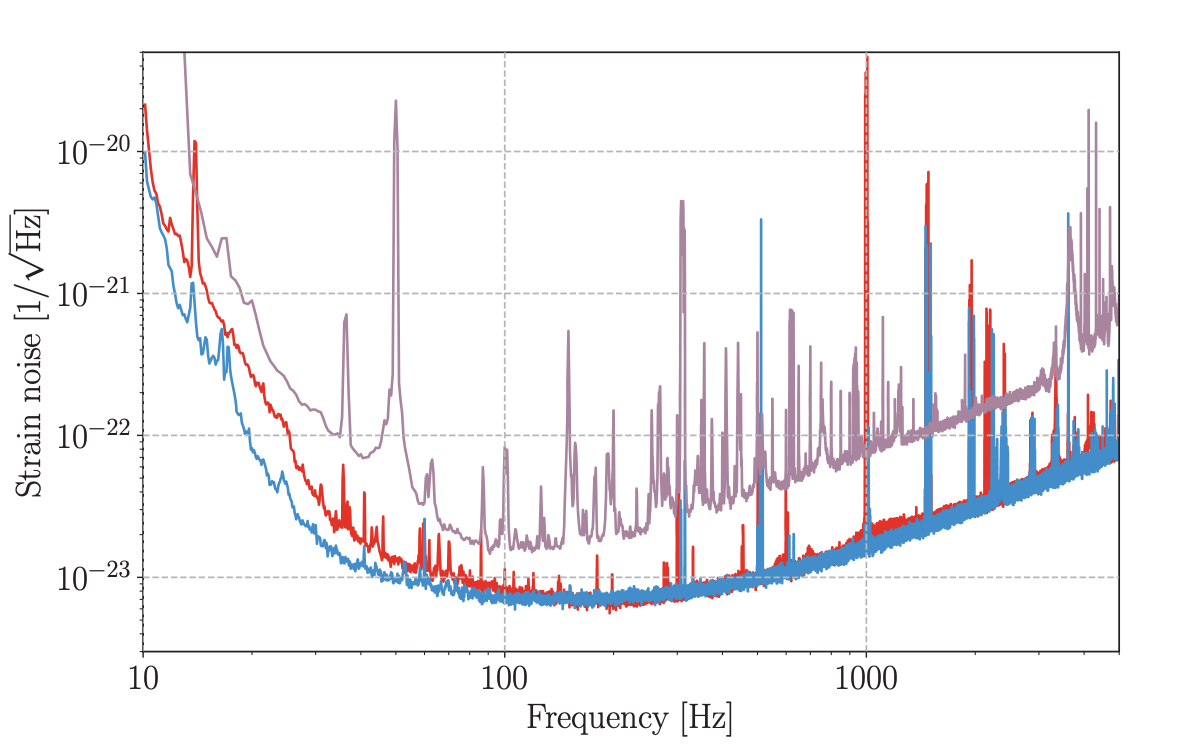
\includegraphics[scale=0.6]{noise1}
                	\centering
                	\caption{Amplitude spectral density of the total strain noise  of the Virgo, LHO, and LLO detectors. The curves are representative of the best performance of each detector during O2 \cite{13}.}
                	\label{fig:noise1}
                \end{figure}

\subsection{Sources}

	There are four different classes of physical sources 
	that are potential sources of GWs 
	of sufficient amplitude to be detectable 
	by current or theorised GW detectors. 

\subsubsection{Coalescing compact binaries}

	Compact binary star systems, in which each member is a NS or BH, 
	are currently the only observed sources of GWs.
	They are an ideal source for ground based GW detectors, 
	as their compactness allows their orbital separation to become 
	small enough before they merge for them to emit GWs in the detectors sensitive frequency band.
	If one of the components of the binary is a NS 
	then there may be an electromagnetic counterpart to the GW signal \cite{20}. 
	The loss of energy from the system will cause the orbital radius to decay, 
	the frequency to increase, and the amplitude of the radiation to increase, 
	producing a distinctive chirp-like signal. 
	Eventually, the two objects will be close enough to merge together, 
	and the new single object will pulsate in an excite state as it tries to return to equilibrium \cite{21}. 
	If the remanant is a BH, this phase is known as the ringdown phase and it is well-modeled as a series of quasi-normal modes. 
	As the form of the gravitational radiation can be predicted allows 
	a more sensitive search to be performed: knowing the form of the signal 
	that is being search for allows powerful matched filtering techniques 
	and signal consistency tests to be used in the attempt to detect such signals.


\subsubsection{Bursts}

	A burst of GWs is an event that releases a large amount 
	of gravitational energy over a very short period of time, typically less than a few seconds.  
	Astrophysical events that are believed to result in a transient signal 
	include gamma ray bursts and supernovae explosion as well as the final stages of a coalescing binary. 
	GW signal with a partially modelled or unknown waveform, 
	this may be due to unknown or complicated physics, or the source may be something totally unpredicted. 
	The matched filtering is not a useful technique to search for this type of signal, 
	as the waveform of a GW burst signal is unknown \cite{3}. 
	Searches for GW bursts typically search for excess power that occurs coherently between multiple detectors.  
	Even with no knowledge of the source of a GW signal, 
	it is still possible to estimate some of the source parameters. 
	Searches for GW bursts typically give estimations of the duration, 
	amplitude and frequency of the source. \\
	An estimation of the sky position is given by measuring the difference 
	in arrival time between different detectors. 
	If the distance to the source is known, 
	perhaps through an electromagnetic counterpart, 
	then it is possible to estimate the energy of the source. 


\subsubsection{Continuous Sources}

	A periodic source is a source that emits at constant or nearly constant frequency.
	The prototypical source of continuous GWs is high frequency rotating NSs 
	with a non-axial deformation or low frequency binary systems 
	composed of white dwarfs or BHs far from merger. 
	These sources should be present throughout the operational lifetime of a detector, 
	so the greater the observation time, the better the sensitivity to periodic sources becomes. 
	Spinning NSs will lose energy and spin down over time, 
	and this energy loss is due to a number of different mechanisms, 
	including emission of gravitational radiation \cite{3}. 
	To emit a continuous GW with characteristic amplitude, 
	a NS must have a non-axisymmetry in the crust. 
	The radiation amplitude is proportional to the crucial parameter $\epsilon$, 
	the fractional asymmetry that is proportional to the mass of the bump on the surface. \\
	As NSs emit electromagnetic radiation, 
	it is possible to target searches of GWs for NSs with positions, 
	frequencies and spin-downs known from X-ray, radio and gamma-ray observations. 
	Examples are the Crab and Vela pulsars. 
	Continuous GWs have not yet been detected, 
	but current searches have produced upper limits for their emission. 
	Upgraded interferometers in LIGO could set an upper limit on  
	$\epsilon$ of order $10^{-6}$ for sources at $\sim10$ kpc, 
	and explain how a NS can be distorted to give a value of $\epsilon$ that is interesting as a GW source. 
	Whatever the mechanism generating the distortion, 
	it is clear that  $\epsilon$ will be small,
	so that $h \sim 10^{-24}$ or smaller, which is quite weak. 
	Measuring these waves will require
	coherently tracking their signal for a large number of wave cycles, 
	which is actually quite difficult, 
	since the signal is strongly modulated by the Earth’s rotation and orbital motion.\\
	Searching for periodic GWs means demodulating the motion of the detector, 
	a computationally intensive problem since the modulation is different for every sky position \cite{4}. 
	Unless one knows in advance the position of the source, 
	one needs to search over a huge number of sky position "error boxes”.

\subsubsection{Stochastic background}

	Stochastic backgrounds are “random” GWs, 
	arising from a  number of sources that overlap 
	in time and frequency that are not individually resolvable \cite{22}. 
	The sum of the signals at any given time and frequency will have 
	a random pattern that may be analyzed statistically but not predicted precisely.
	A particularly interesting source of stochastic waves is the dynamics of the early Universe, 
	which could produce an all-sky GW background, 
	similar to the cosmic microwave background. \\ 
	However, to measure waves from this epoch, 
	we would need much more sensitive detectors than the ground-based interferometers available.
	Stochastic backgrounds are usually idealized as being stationary, 
	isotropic and homogeneous and because of their random nature they look just like noise \cite{4}.	
	Another possible background could come from astrophysical sources. \\ 
	These possible sources include a population of rotating NSs 
	and a population of white dwarf binaries that would be important mostly for a space-based interferometers such as LISA. 

%----------------------------------------------------------------------------------------------------------------------------------------------------------------------------------------------------------
\chapter{Data Analysis for Coalescing Binary Systems}

	One of the tasks of GW data analysis is to extract GWs signal 
	buried into noisy interferometric strain data, hence achieving GW detections.
	The techniques involved in this proces depend on the type of source.
	GW searches from the inspiral, merger and ringdown phases of compact binary systems 
	are based on two broad techniques: 
	modeled searches which use theoretical waveforms for the GW emitted by such systems 
	as predicted by general relativity, and 
	unmodelled (or burst) searches which assume minimal information about these waveforms \cite{23}.
        This chapter provides a basic overview of the main data analysis ingredients needed to perform a modelled GW search:
        matched filtering, template banks, evalution of a candidate's significance, measure of the sensitivity of a search.

\section{Matched Filtering}
	Although signals from coalescing binaries will most probably not stand above the broadband noise of the detector, 
	their detection is possible by the use of matched filtering, 
	which takes advantage of the fact that the waveform can be fairly well predicted. 
	As we will see, this technique is the optimal detection strategy when searching for GWs
        with well understood waveforms in Gaussian noise.

	The filtering procedure involves correlating the detector output 
	with a copy of the expected waveform, 
	called template.
	A real detector operates over a finite frequency band, 
	and acquires data at a finite sample rate \cite{24}. 
	In this case, the noise power spectrum $S_n$ 
	may be taken to be infinite outside the bandwidth of the instrument, 
	effectively restricting the range of integration to lie between $[-f_N, f_N]$, 
	where $f_N$ denotes the Nyquist frequency $f_N = 1/(2\Delta t)$, 
	and $\Delta t$ is the time between successive data samples.   \\
	The measured detector strain amplitude, $s(t)$, may or may not contain a signal,
	thus it will be composed of $n(t)$, the real strain-equivalent noise
        produced by fluctuations within the detector and its environment, 
	and possibly a GW of known form, $h(t)$
                \begin{equation}
                        s(t) = h(t) + n(t)\,.
                \end{equation}
        When no signal is present,   		
		\begin{equation}
                        s(t) = n(t)\,.
                \end{equation}
        The aim of the match filtering is to look for a filter function to process the data,
	the output of which will be large when a signal is present and small otherwise. 
        If the waveform, $h(t)$, is embedded in stationary Gaussian noise with zero mean and one-sided power-spectral density (PSD) $S_n(f)$,
        the optimal filter takes the form $\tilde h_{template}/S_n$, where $\tilde h_{template}$
        is the frequency domain waveform template that approximates the real signal to the best of our knowledge.
	This optimal filter may be cross-correlated with the data over the detector frequency band to search for GW
        signals.  The output of this filtering operation may be viewed as a weighted inner product in the frequency domain, 
	between the data and the template, where the weight is the inverse PSD of the detector:
		\begin{equation}
 			(s|h)(t) = 4Re \int^{f^{high}}_{f^{low}} {{\tilde s (f) \tilde h^{*}_{template}(f)} \over {S_n (f)}} e^{2 \pi ift}df\,, 
		\end{equation}
	where the frequency limits $f_{low}$ and $f_{high}$ are determined by the detector bandwidth
	and $\hat s(f)$ denotes the Fourier-transformed detector data, defined as
		\begin{equation}
			\tilde s(f) = \int^{\infty}_{-\infty} s(t) e^{-2i \pi tf} dt\,.
		\end{equation}
  
\subsection{Signal-to-noise ratio}

	Finding the form of the filter which will optimally extract the signal from the noise,
        means locating the maxima of the output of the matched filter, $(s|h)(t)$, 
	over the arrival time and phase.
        One can therefore set a threshold value such that values of the matched filter 
	above it would indicate a signal candidate while values below would indicate the absence of signals. \\
	The filter output can be normalized by the variance of the optimal filter, $\sigma^2$,
	which is an estimate of the uncertainty in a measurement of $(s|h)$ due to the detector noise:
                \begin{equation}
                        \sigma^2 =4 \int^{f^{high}}_{f^{low}} {{|\tilde h_{template}(f)|^2} \over {S_n(f)}}df
                \end{equation}
 	The normalized output of the optimal filter is a new thresholding statistic and can be defined as  
	the signal-to-noise ratio (SNR), the ratio of the observed filter output to its,
        expected or observed, root-mean-square fluctuations \cite{24}:
                \begin{align}
                        \rho(t) &= {{| (s|h) |} \over {\sigma_{h}}} \\
                             &= {{(\tilde s|\tilde h_{template})} \over {\sqrt{(h_{template}|h_{template})}}}\,.
                \end{align}
        The value of the SNR will then be proportional to the amplitude of the signal buried in the noise.
	The smart choice for a threshold that can be set on this value is such that
	it can admit as many signals as possible, while still keeping the false alarm rate low. 

\subsection{Matched filtering for compact binary coalescence signals}

	An interferometric detector is sensitive to a linear combination 
	of the two GW polarizations \cite{26}: 
                \begin{equation}
                h(t) = F_{+}h_{+} (t) + F_{\times}h_{\times}(t)\,,
                \end{equation}
	where $F_{+}$ and $F_{\times}$ are the two antenna response functions of the detector, 
	which depend on $\theta$ and $\phi$, 
	the angular coordinates of the source sky position with respect to axes defined by the interferometer arms. 
	Due to the nature of GW signals from the inspiral stage of compact binary coalescences (CBCs), 
	it follows that the phase evolution of the cross polarization is $\ang{90}$ out of phase with the plus polarization:
		\begin{equation}
			h_{+}(t) = A(t) \cos (\phi (t))
		\end{equation}
		\begin{equation}
			h_{\times}(t) = A(t) \sin (\phi (t))  
		\end{equation}
	where $A(t)$ is the amplitude evolution of the signal 
	and $\phi(t)$ is the phase evolution of the signal. 
	The Fourier transform of the two polarization are related by $\tilde h_{+} = i\tilde{h}_{\times}$, 
	which means that the inner product between the two orthogonal polarisations is zero 
		\begin{equation}
			(h_{\times}|h_{+}) = 0
		\end{equation}
	Hence, when filtering  $s = (Xh_{+}/\sigma_{h}) + (Y h_{\times}/\sigma_{h})$ 
	with the templates $h_{+}$ and $h_{\times}$, we obtain the matched-filter real-time series
		\begin{equation}
			z_{+} = X\sigma_{h}
		\end{equation}
		\begin{equation}
			z_{\times} = Y \sigma_{h} 
		\end{equation}
	This leads to the definition of the two-phase filter, 
	which has twice the degrees of freedom of a single-phase filter:
		\begin{equation}
			\rho = {1 \over \sigma_h} \sqrt{|z_{+}| ^2+ |z_{\times}|^2}
		\end{equation}
	The bonus of extracting information from both polarizations of the GW 
	comes at the cost of increasing the expectation value of $\rho$ when there is no signal present. 
	For a detector output that includes a signal at distance $D_{eff}$, 
	$s(t) = n(t) + (D_{eff}/1 Mpc)^{-1}h_{1Mpc}$, 
	a biased estimate of the effective distance for a given trigger 
	may be defined by combining the definition of the SNR with the template normalization $\sigma_h$:
		\begin{equation}
			\hat D_{eff} = {{\sigma_h} \over {\rho}}
		\end{equation}
	In reality, the parameters of astrophysical systems will not be known a-priori, 
	and searches must therefore be sensitive to signals at any location in the parameter space \cite{25}. 
	Performing the matched-filter calculation at every point in the full parameter space 
	would be computationally prohibitive, 
	and therefore a number of analytic approximations are used to reduce the size of the parameter space. 
	It is assumed that the ``extrinsic'' parameters of a GW signal --- 
	sky-location, source orientation, polarisation phase and distance --- 
	can all be absorbed by applying a constant phase-shift, 
	constant time-shift and a constant amplitude scaling to the observed waveform \cite{27}. 
	With these assumptions in place, 
	one can analytically maximise over an overall amplitude and phase of the signal, 
	and use an inverse Fourier transform to quickly evaluate the statistic as a function of time. \\
	The component masses and spins --- the intrinsic parameters --- 
	are searched over by repeating the search process with a well chosen discrete set of waveform models 
	with varying values of the component masses and spins, 
	known as the template bank \cite{27}. 
	Physically, these assumptions hold if one assumes that the sources being observed 
	have negligible orbital eccentricity, precession and contributions from higher-order modes 
	to the GW signal \cite{23}. 

\section{Template Banks}

	To perform a matched-filtered search that recovers compact binary coalescence signals
	with minimal loss of SNR over a given range of intrinsic parameters, 
	one must filter the data against a predetermined collection of waveform models: the template bank \cite{28}.
	The manifold of waveforms is a continuous space in the component masses and spins. 
	One may only to search over this manifold on a discrete points, 
	which have to be placed in such a way that any signal
	that has parameters in the targeted space will still produce an SNR 
	above threshold by matching with the ''losest'' template \cite{27}. \\ 
	In order to compute the distance between two templates with different parameter values, 
	one can create a metric over the parameter space and then compute an ``error'' between two waveforms.
	Two neighbouring templates can be defined as $\tilde h(f;\lambda)$ and $\tilde h(f;\lambda + \Delta \lambda)$,
	where $\lambda = \{\lambda_{intr}, \lambda_{extr}\}$ is the set of 
	intrinsic (masses and spins) and extrinsic (time and phase shifts) template parameters.
	Using the overlap of two waveforms, defined as the normalized inner product inversely weighted 
	by the detector one-sided PSD $S_n(f)$, one can define the match:
		\begin{equation}
			\mathcal{M}(\lambda, \Delta \lambda) \equiv \max_{\Delta \lambda_{extr}} (\tilde h(f;\lambda), \tilde h(f;\lambda + \Delta \lambda))
		\end{equation}
        \fpg{Qua manca la normalizzazione.}
	The match is maximised only over the two extrinsic parameters of a template, 
	because waveforms related by time and phase offsets
	are described by the same template, 
	since all possible coalescence times and phases are searched for \cite{29}. \\
	This expression can be Taylor-expanded about $\Delta \lambda = 0$:
		\begin{equation}
			\mathcal{M}(\lambda, \Delta \lambda) \simeq 1 - g_{ij} \Delta \lambda^i \Delta \lambda^j\,,
		\end{equation}
	where 
		\begin{equation}
			 g_{ij} \equiv -{1 \over 2} {{\partial^2\mathcal{M}} \over {\partial  \Delta \lambda^i  \partial \Delta \lambda^j}}\vert_{\Delta \lambda = 0}
		\end{equation}
	can be interpreted as a metric in the waveform manifold.  A commonly used quantity related to this metric
	is the mismatch between two templates $MM = (1 − \mathcal{M})$.
	Any mismatch between signal and template leads to a loss in SNR, 
	and to a down-weighting by the signal-based vetoes \fpg{(see Sec.\,...)}. \\
	When constructing a template bank, this mismatch can be viewed as the means
	to compute the proper distance in the waveform space:
		\begin{equation}
			ds_{ij}^2 = 1 − \mathcal{M} = g_{ij} \Delta \lambda^i \Delta \lambda^j\,.
		\end{equation}
	This proper distance should be chosen to guarantee that the loss in SNR due to the mismatch 
	between template and signal does not jeopardize the detectability of the signal \cite{30}.

\subsubsection{Fitting factor}

	The standard measure used to determine the set of waveform models to used in a
        search is the fitting factor, $FF$.
	The fitting factor quantitatively describes the ``closeness'' of 
	the true signals to the template manifold, in terms of the fraction of 
	SNR obtained when filtering 
	the data with an approximate family of templates \cite{31}. 
	To quantify the bank coverage, usually Monte-Carlo simulations are carried out   
	to compute the distribution of fitting factors of the templates in the bank against 
	a set of injected signal waveforms with randomly chosen parameters \cite{32}. \\
	The fitting factor, $FF$, of a template bank with respect to an injected signal $h_{*}$ 
	is defined as the maximum value of match over all the templates:
		\begin{equation}
			FF(h_{*}) = \max_\Lambda \mathcal{M}(\tilde{h}_{*}, \tilde{h}(\Lambda))
		\end{equation}
	assuming that the signal model is the same for both templates and injections. 
	The fractional loss of SNR in capturing the signal 
	$h_{*}$ with the template bank is $1 - FF(h_{*})$.
	If the fitting factor is less than unity, the signal lies outside the parameter space, 
	and the fitting factor represents the cross-correlation between 
	the signal and its nearest template in the waveform parameter space \cite{33}. 
	This loss arises from the discrete placement of the templates. 
	Because binaries are, on large scales, uniformly distributed in space 
	and because the signal strength scales inversely with distance, 
	the fraction of events retained is approximately $FF(h_*)^3$. \\ 
	Therefore it is desirable that the template bank is constructed such that 
	no putative signal anywhere in the parameter space
	has a FF value less than the minimal match. 
	A bank is said to be effectual if it can satisfy this condition.
	It has become conventional to set $FF = 97\%$ as a reasonable goal when building a template bank, 
	as this translates into a $10\%$ loss of events \cite{33}.

\subsubsection{Frequency bound}

	An algorithm that most efficiently covers the parameter space relies on the choice of a coordinate system, 
	in which the metric is as flat as possible across the space \cite{34}.
	In computations with the two-mass-parameter waveforms, 
	the best coordinates to use on the parameter space are not the two masses, 
	but rather the inspiral times, chirp times, from some fiducial frequency to final merger, 
	as computed at Newtonian and first post-Newtonian order. 
	The metric components are slowly varying over the parameter space, 
	when expressed in as dimensionless chirp times. 
        The lower frequency cutoff $f_L$, which essentially determines the size of the parameter space
        of chirptimes and plays a crucial role in the computational resources required
        to process the data through the template bank \cite{30}, and is not itself a parameter to search for. \\
        However, it affects the length of the signals
        (therefore, the parameter space to be covered) and the SNR extracted.

\subsection{Template placement}

	The computational cost of any GW search
	 is directly proportional to the number of templates used \cite{28}.
	It is therefore vital to have a method that enables one 
	to place a template bank using as few templates as possible. \\ 
	Two broad classes of template-placement algorithms 
	have been developed in the literature. 

\subsubsection{Stochastic placement}

	Stochastic methods place templates, 
	that are randomly drawn from an initially chosen distribution, 
	at random points in the parameter space.
	The bank is gradually built by comparing the newly drawn waveform
	with previously accepted templates, 
	and keeping only the ones that are sufficiently far away 
	from the ones already in the bank.
 	Those that are too similar to at least one existing waveform are discarded \cite{35}.
	This procedure continues until the pre-set convergence threshold is reached, 
	resulting in a final saturated template bank.
	The threshold is measured from the ratio of rejected templates over the total number of template candidates.
	Stochastic placement, however, has the shortcoming that 
	a large number of trial waveforms needs to be drawn and generated before convergence is achieved 
	(many more than the required number of templates in the bank). 
	This method also tends to over-cover the parameter space, 
	in the sense that the average template density is higher than optimal at fixed minimum match. \\
	Furthermore, the construction of a stochastic template bank 
	can be computationally demanding since, in principle, 
	each new proposed template needs to be compared 
	with the previously chosen templates \cite{36}. 
	This problem becomes particularly acute 
	the closer the bank gets to saturation. 
	The computational problem also becomes especially demanding 
	when precession effects are considered as these additional degrees 
	of freedom require a large number of templates. \\
	It is therefore important to consider methods to optimise the template bank construction, 
	specifically finding ways of improving effectualness for a given number 
	of templates and reducing the computational cost. 

\subsubsection{Geometric placement}


	A different method to construct the bank is geometric placement:
	this means building a flat, linear space in such a way that embeds the space of physical waveforms. 
	Hence, a crucial point is to identify a set of coordinates 
	in which the parameter space metric is almost constant: 
	the Euclidean distance in this space coincides with the matched-filtering overlap 
	between waveforms, making these coordinates naturally suited to define a regular lattice. 
	The minimal match determines the choice of spacing of the discrete template parameters, as shown in Section 3.2, 
	and therefore the number of discrete templates in the family.
	The most significant drawback of such banks is the amount of fine-tuning required 
	in order to cover ``holes'' across local patches because of the misalignment 
	of the cells arising from the variation of the metric \cite{29}. 

\subsubsection{Hybrid placement}

	In practice, a combination of the two methods is often a better strategy. 
	For example, one can place templates geometrically at low masses 
	and stochastically at high masses, or one can use many small patches 
	with regularly spaced templates, which are themselves placed stochastically 
	to cover the entire parameter space \cite{29, 34}. 

\subsubsection{Spins of compact objects}

	The processes that lead to the formation of a compact binary
	depend sensitively on a number of poorly constrained parameters, 
	such as the typical stellar metallicity at formation, 
	the distribution of supernova kicks, 
	and the binding energy of the common envelope. 
	There are two main channels through which compact objects can be formed:
	the coevolution of two massive stars in a binary and 
	the dynamical capture of two preformed compact objects 
	in dense stellar environments such as globular clusters \cite{37}. \\	
	It is thought that compact binaries formed by dynamical capture 
	are more likely to have component spins
	at large angles with respect to the orbital angular momentum, 
	while those formed by common evolution are more likely to have 
	spins that are nearly aligned with the orbital angular momentum.
	Present observations clearly indicate the potential for large spins 
	on BHs in binaries, possibly close to the Kerr limit $|\mathbf{S}/m^2| = |\mathbf{\chi}| = 1$.
	Very few measurements of the angles between the spins and 
	the orbital angular momentum exist from electromagnetic observations. 
	In some cases, one can measure this spin misalignment via GW emission, 
	as misalignment leads to precession of the orbital plane, 
	which appears as phase and amplitude modulations in the observed signal. \\
	Almost all searches for GWs from coalescing compact binaries 
	using the data of first generation interferometers 
	have used templates that neglect the spins of the compact objects \cite{32}.
	This was primarily motivated by the sensitivity of the initial LIGO and Virgo detectors:
	because the sensitivity band started above 40 Hz, 
	including spin effects greatly increased the number of templates to be searched over, 
	and the search performed, on average, no better than non spinning searches, 	
	as the increased degrees of freedom in the signal space picked up extra noise noise transients, 	
	increasing the false alarm rate \cite{32, 38}. \\ 
	However, the Advanced LIGO and Virgo detectors are sensitive to frequencies above 10–20 Hz, 
	therefore they can observe the inspiral from much larger orbital separations, 
	resulting is significantly longer observed GW signal \cite{23}. 
	Proper consideration of the spin effects is essential in the advanced detector era, 
	as there might be astrophysical systems that are entirely missed by non-precessing searches.
	Neglecting the spin effects can cause a much larger dephasing of the template with the signal, 
	and hence considerable loss of SNR. \\
	Currently, waveform models with spins (anti)aligned with the orbital angular momentum 
	are used in searches with Advanced LIGO and Virgo, 
	as it was demonstrated that aligned-spin templates accumulate more signals than noise \cite{27}. 
	While building a template bank with the geometric approach for these cases is feasible, 
	since a closed-form expression of the template-space metric can be computed, 
	this is not possible for binaries with generic spins. 
	This is due to the fact that, 
	if the spins are misaligned with the orbital angular momentum of the binary, 
	the spin-orbit and spin-spin interactions will cause the spins 
	(and hence the orbit) to precess. 
	The resulting dynamics as well as the GW forms are rather complex, 
	and the modelling requires solving a set of coupled ordinary differential equations \cite{39}. 
	The template placement is further complicated by the large dimensionality of the parameter space 
	(two mass parameters, five spin parameters, and two angles describing the orientation of the binary, in general). 
	Detecting highly precessing systems offers a better chance to 
	disentangle the various parameters that describe the source,  
	breaking degeneracies that exist between physical parameters 
	in the emitted GW signal.  
	This could allow for a better understanding of the nature and origin of these systems.
	Although the effect of precession on the GW signal is not fully captured 
	by aligned-spin templates, it has been demonstrated that non-precessing templates 
	are also effectual in detecting binaries with generic spins if the mass ratio is moderate 
	$(m_1/m_2 \leq 10)$; these spin effects can be also described by 
	a single reduced-spin parameter in an approximate way, 
	which makes the parameter space three-dimensional, 
	using the two masses and reduced-spin as variables \cite{32}. 
	
\section{Candidate ranking statistic}

 	Since the detector calibrated strain data contains both stationary, Gaussian noise
        and non-Gaussian noise transients of instrumental and environmental origin,
        matched filtering does not suffice as a detection statistic.
        Consistency checks are needed to mitigate the effect of noise transients,
        which can sometimes mimic signals of astrophysical origin,
        and to assign an accurate statistical significance to candidate signals.
        In order to eliminate the worst periods of detector performance, 
        data quality investigations are conducted by looking only at the detector behaviour,  
        which is analysed by monitoring environmental and instrumental channels \cite{40}.
        After removing data that is not suitable for astrophysical searches, 
        noise transients, glitches, of unknown origin could still be present in the data 
        and cause certain templates to produce high SNR values.
        To mitigate the effect of glitches, a gating procedure is applied:
        after identification of times impacting on the sensitivity of the search,
        the data are zeroed out around these times \cite{42}.
        Filtering the data with template banks generates a matched-filter SNR for each template in each detector;
        GPS times of local maxima that exceed the SNR threshold are recorded as triggers. 
        Waveform consistency tests are then needed to determine if the morphology 
        of a candidate signal is consistent with the expectation from the triggering template waveform.  If it is not,
        it is more likely to correspond to a noise transient.
	
\subsection{$\chi^2$ test}

	For signals from compact binary mergers, one can construct $\chi^2$-test.
	A standard $\chi^2$-test consists in splitting the template into $p$ non-overlapping frequency bins 
	constructed so that each one contributes equally to 
	the SNR of a perfectly matching signal \cite{28, 41}. 
	The $\chi^2$ statistic compares the expected to the measured SNR in each bin as follows:
		\begin{equation}
			\chi^2_r = {1 \over {2p-2}}   \sum_{i=1}^{i=p} || \langle   s|h_i  \rangle -   \langle  h_i|h_i   \rangle ||^2\,,
		\end{equation}
	where $\chi^2_r = \chi^2/(2p-2)$ is the reduced chi-squared.  For real GW signals, this value should be close to unity, 
	meaning that the data is describing Gaussian noise with an embedded signal.\\
	The SNR returned by the matched filtering procedure is combined with the $\chi^2$-test result to produce a ranking statistic 
	that down-weights triggers caused by noise transients, the so-called reweighted SNR:
		\begin{equation}
		\begin{cases}
			\hat \rho &= \rho \hspace*{4.5cm}  \text{for} \hspace*{0.15cm}\chi^2_r \leq 1 \\
			\hat \rho &= \rho[{1 \over 2} (1 + (\chi^2_r)^3)]^{-1/6}  \hspace*{1.5cm}  \text{for} \hspace*{0.15cm} \chi^2_r > 1
		\end{cases}
		\end{equation}
                \fpg{Quello che segue riguarda i consistency tests, non i chi-square tests.} 
	The search requires that GW signals be identified via matched filtering 
	in at least two independent detectors with consistent parameters. 
	To be considered a candidate event, arrival times of the GWs at each detector 
	must differ by no more than the the maximum time-of-flight between the detectors, 
	with an additional window to account for uncertainty in the measurement of the time of arrival \cite{13}.
 
\subsection{False Alarm Rate}

\fpg{Sono qui.}

	After mitigating the effects of noise transients, the probability of remaining transients 
	occurring simultaneously in two detectors and producing a large joint 
	ranking statistic value becomes extremely small.
	In order to keep only the most representative trigger among all the triggers produced by a single inspiral signal or glitch, 
	a final clustering step is performed on coincident triggers, 
	by selecting those with the largest value of $\hat \rho$ 
	in each time window of $10s$. 
	Any other events in the same time window are discarded. 
	This ensures that a loud signal or transient noise artifact gives rise to at most one candidate event.
	In order to assess the actual significance of a candidate, 
	we need to measure the false-alarm rate, (FAR), of the search as a function of the detection statistic.
	Typically, a detector’s background FAR can be determined 
	simply by turning off the source or changing the orientation of the detector \cite{13, 43}. \\ 
  	However, since it is not possible to isolate the detectors from GWs, 
	it is impossible to directly measure the detector noise in the absence of signals.
 	To estimate the FARs the data stream is shifted in time, 
	choosing the minimum time-shift offset to be larger than the time-coincidence window 
	used to determine if signals are observed with consistent parameters in the network.
	The resulting “time-shifted” coincidences are then treated as a background noise sample, as seen in Fig.$\ref{fig:Significance}$. 
	This is done numerous times with different time shifts in order to obtain 
	a probability distribution for the joint detector ranking statistics \cite{44}. 
		\begin{figure}[H]
			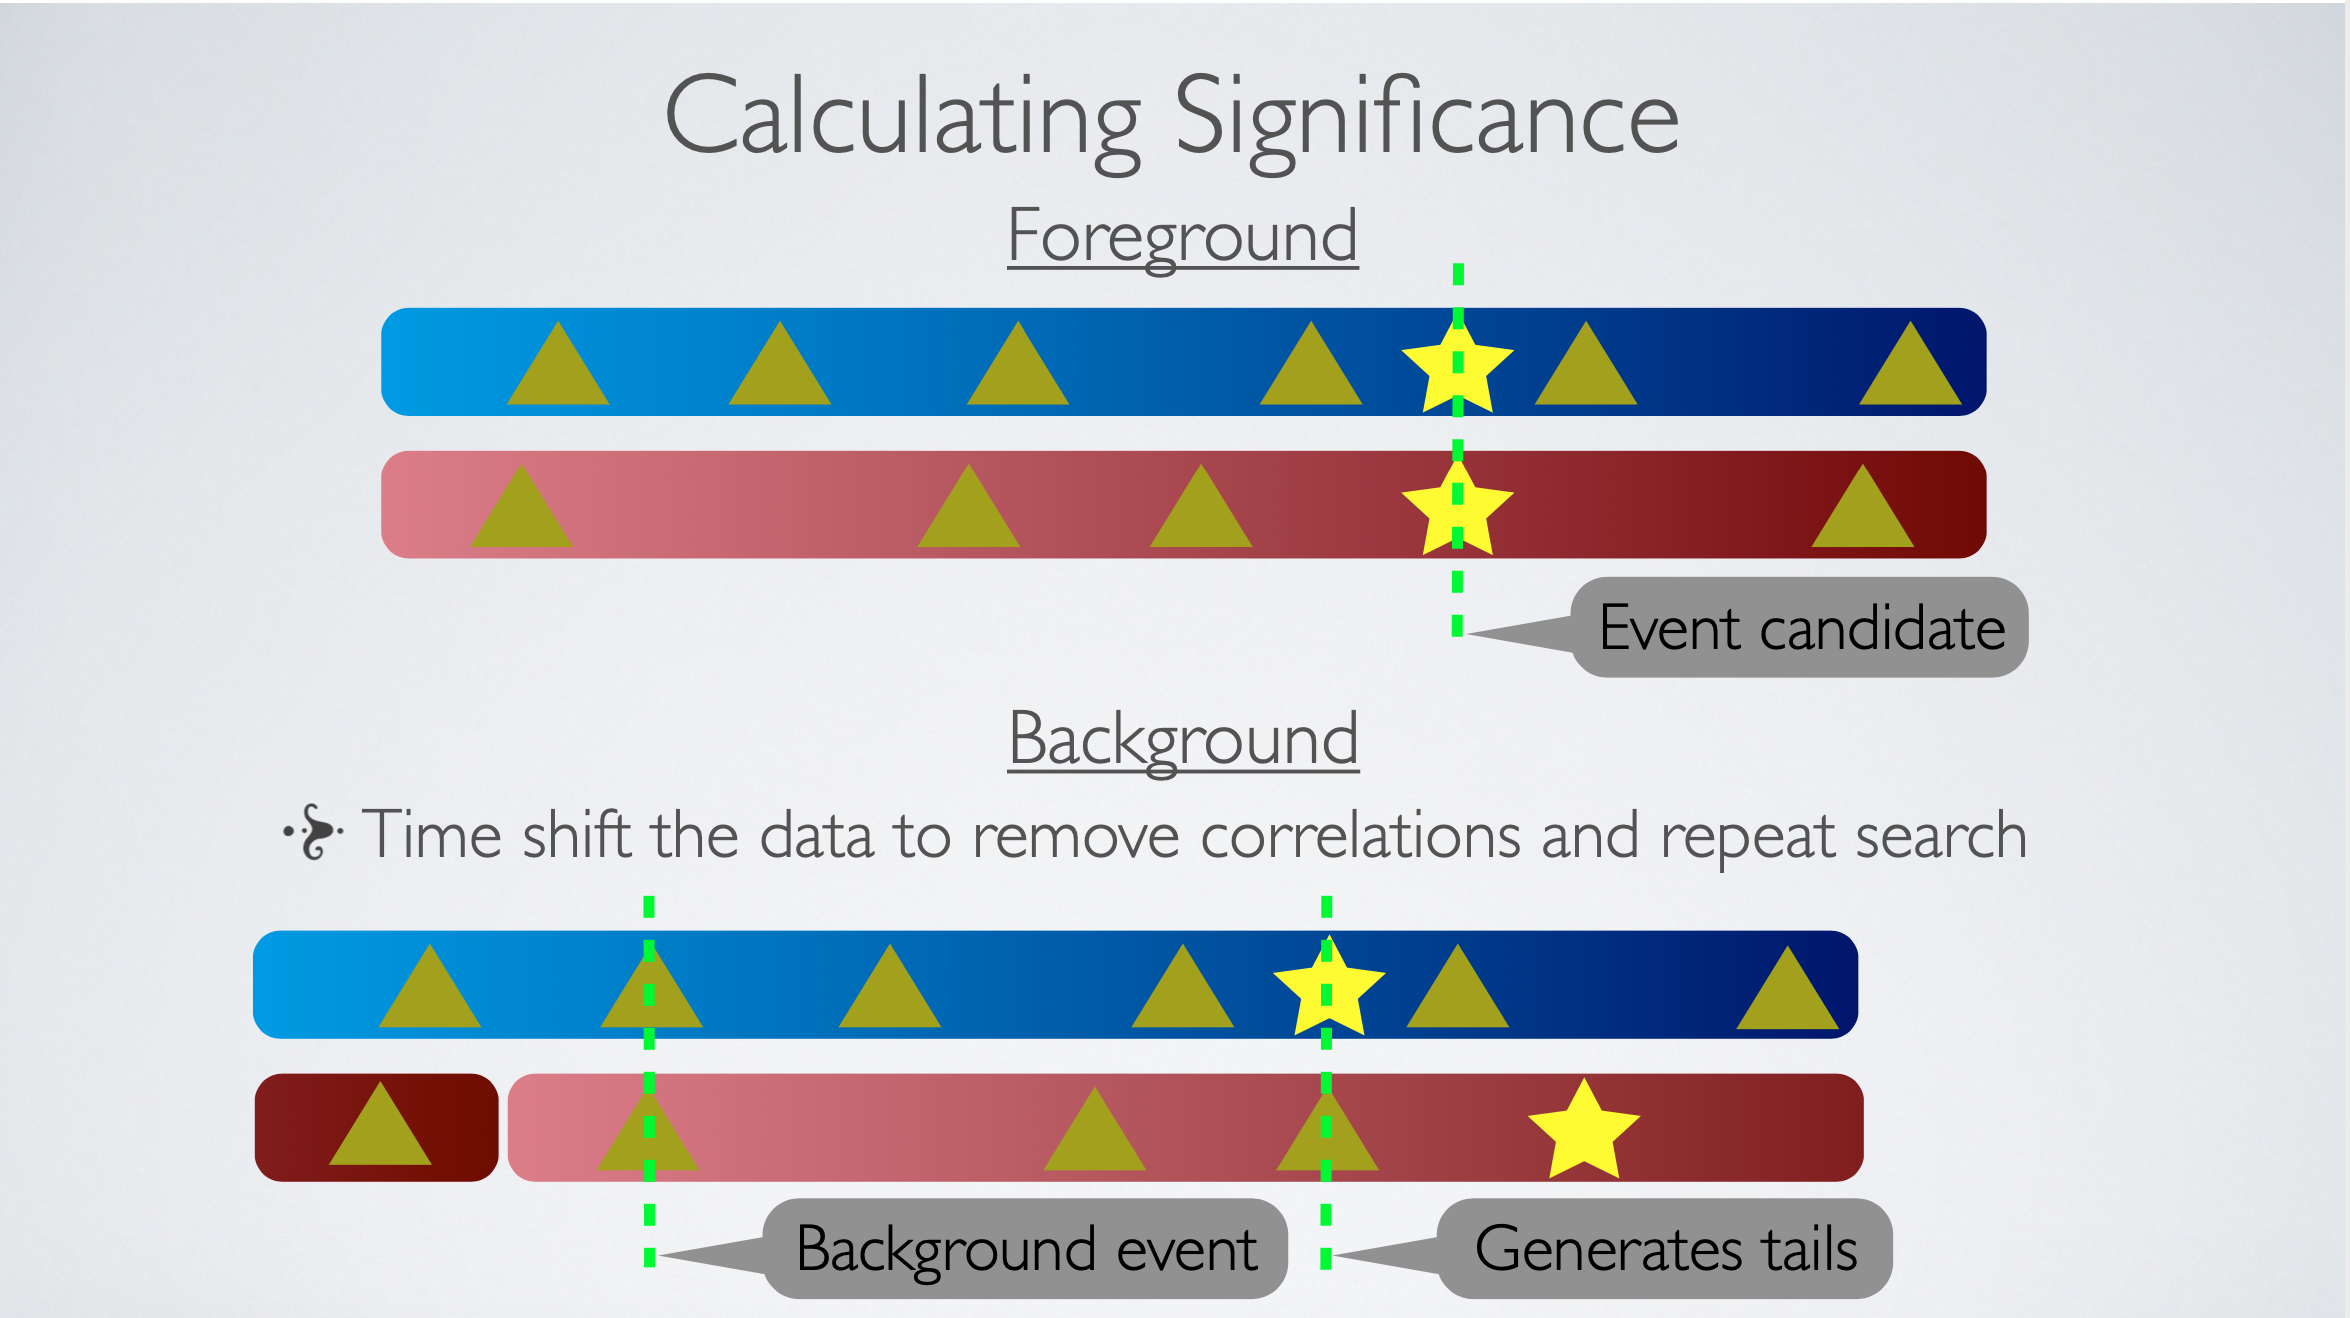
\includegraphics[scale=0.25]{Significance}
                  	\centering
                  	\caption{Visual description of time shifting data to build a background noise sample.}
                  	\label{fig:Significance}
                 \end{figure}
	Each coincident trigger is assigned a FAR given by the number 
	of background triggers, $n_b(\hat \rho)$, with an equal or larger ranking statistic, 
	divided by the total time searched for time-shifted coincidences $T_b$
		\begin{equation}
			FAR = {{1 + n_(\hat \rho)} \over {T_b}}
		\end{equation}
	To account for the noise background varying across the target signal space, 
	candidate and background events are divided into different search classes based on template length. 
	The significance of candidate events is measured against the background from the same class. 
	For each candidate event, one can compute the probability of finding one or more 
	noise background events in the observation time with a detection-statistic value above that of the candidate event, given by 
		\begin{equation}
			FAP(\hat \rho) \equiv P(\geq 1 \hspace*{0.1cm}\text{noise event above}\hspace*{0.1cm} \hat \rho|T,T_b) = 1 - e^{-T{{1+n_b(\hat \rho)} \over{T_b}}}
		\end{equation}
	where T is the observation time of the search.
	If a candidate event’s detection-statistic value is larger 
	than that of any noise background event, 
	then the analysis places an upper bound on the candidate’s false alarm probability. 
	The inverse of FAR specifies the waiting time before such an event from noise is seen, and it is given by 
		\begin{equation}
			IFAR = {1 \over {FAR}}
		\end{equation}   
\section{Coincident and coherent research}

	There are two main detection strategies to search for GWs 	
	from a network of detectors: coincident and coherent.

\subsection{Coincident analysis}

	A coincidence analysis searches the data from individual detectors independently 	
	and matches the candidate event lists of individual detectors for consistency,
	in the mass and time parameters of a GW signal.
	This methodology ignores the phase information at the expense of some loss in sensitivity, 
	so there is no guarantee that the observed signals in each detector 
	are compatible with a GW source with two polarisations.
	The benefit of the coincidence search is that it is not computationally expensive: 
	the dominant cost of the search is in performing a matched filter 
	of the data against a bank of template waveforms, (as seen in Section 2.1):
        this task is done once per detector per template \cite{28, 45}. \\
	A search over the sky location of the signal is then trivially done 
	by time-shifting the results from the different detectors accordingly.
        Similarly, the noise background is estimated by applying larger time shifts to the data,
        significantly longer than the light travel time between detectors, to search for noise coincidences.
        In a coincidence search, it is necessary to place a threshold on the SNR of events
        which will be stored by the analysis prior to identifying coincidences.
        This means that the power in the GW signal will only be accumulated
	in those detectors where there was an event above threshold \cite{45}.

\subsection{Coherent}

	A coherent search is a very sensitive way to search for GWs from a network of detectors:
	this strategy treats the detectors as if they are isolated 
	and then combines the data from all detectors phase coherently, 
	appropriately correcting for time-delays and polarization phases, 
	to obtain an individual detection statistic which is then compared with a single threshold \cite{18}. 
	The aim of this type of search is to obtain a single statistic for the full 
	network, that is optimized in the maximum likelihood sense, 
	to effectively construct a single, more sensitive detector. \\
 	While this method has been applied to searches for unmodelled burst sources,
        it has proven more difficult to use for the binary merger search \cite{45}.

\subsubsection{Coherent SNR}
	
	The GW signal seen by detector $X$ is a combination of 
	the two polarisations weighted by the detector antenna 
	response
		\begin{equation}
			h^X(t) = F_{+}^X h_{+}(t^X) + F_{\times}^X h_{\times}(t^X) 
		\end{equation}
	where the time of arrival in detector $X$ depends upon the sky location 
	of the source relative to the detector and the time of arrival at a fiducial location, 
	for example the Earth’s centre \cite{45}. 
	For a network of detectors, the multi-detector matched-filter
	is defined as the sum of the single detector inner products
		\begin{equation}
			(a|b) \equiv \sum^D_{X=1} (a^X|b^X)
		\end{equation}
	where D is the number of detectors in the network. The multi-detector log-likelihood is then calculated as
		\begin{equation}
			ln \lambda = (s|h) - {1 \over 2} (h|h)
		\end{equation}
	The larger the value of $ln \lambda$, the more likely that a signal is present.
	The coherent SNR is obtained by maximising the log-likelihood 
	over the values of the waveform amplitudes:

		\begin{equation}
			\rho^2 _{coh}\equiv 2 ln \lambda |_{MAX}
		\end{equation}
	In the absence of a signal, the $\rho^2_{coh}$ follows a $\chi^2$ distribution. \\
        While in a coincidence search requires a signal to be observed in two or more detectors, 
	resulting in the coincident SNR to be simply the sum of all power consistent with the template waveform in each detector,
	the coherent search naturally incorporates the SNR from all operational detectors \cite{45, 46}. \\
	It has been demonstrated that for a signal in the absence of noise the coincident and coherent SNRs are identical. 
	For noise events, the coincident SNR includes all of the noise, 
	while the coherent SNR, incorporating only those contributions which are compatible 
	with a coherent signal at all detectors, obtains precisely the same signal but reduces the noise background \cite{45}. \\
	Even though the coherent method is highly effective at removing background noise,  
	signal consistency tests are still required to distinguish glitches from GW signals. 

\subsubsection{Null Stream Consistency}

	In the coherent analysis the data from all detectors 
	is combined to extract the two physical GW polarisations, 
	and uses this to restrict the signal model to 
	only two independent polarizations, 
	thus it is easier to distinguish transients from GW signals, 
	as those transients which do not contribute power to the signal space, and to reject incoherent background noise. \\
	Consequently the search is more sensitive as the number of detectors in the global network increases.
        When there are more than two detectors, 
	it is possible to construct one or more null data streams 
	which contain only noise, and define the null SNR as
		\begin{equation}
			\rho^2_N = \rho^2_{coinc} - \rho^2_{coh} 
		\end{equation}
	Requiring a small null SNR is an effective method to separate 
	an incoherent noise transient from a real GW signals: 
	in fact such noise events may give a large coherent SNR,
	but it is likely to also give a large null SNR \cite{45}.       

\section{Injections}

	In order to test the sensitivity of a search pipeline to detect CBC signals, 
	simulated gravitational waveforms, injections, can be added in the data before filtering.
	Then a search can be performed over the data with the added injections just as it would normally do with the real data;
	by determining FARs for the injections that we recover, 	
	and noting which injections are not recovered at all,
	we can understand how well we detect certain types of sources \cite{47, 48}.
	Studies of injection recovery also aid with tuning different parameters 
	of the search pipeline and setting upper limits on the rates of particular sources. 
	One method of determining sensitivity to particular injections is the efficiency, 
	or fraction of found injections, as a function of injected physical distance. 
	Another method of determining a search’s sensitivity to a particular source 
	is to examine the injected distance as a function of frequency 
	(or total mass) for missed and found injections. \\
	These simulations can be performed in two ways: software and hardware injections.
	The former are used to verify the results obtained from software injections, 
	the latter are used for high-statistics evaluation of the performance of analyses \cite{49}. 

\subsection{Software injections}

	Software injections are a streaming time series of simulated gravitational waveforms, 
	generated in the software, from a synthetic population of a certain type of source, 
	described by astrophysical parameters, including the strain amplitude, sky location, 	
	and initial frequency, and added to the data stream \cite{30}. 
	This can be done many times, by specifying a time-step at which to place injections, 
	without disturbing the detector or significantly reducing the duty cycle of the detectors. 
	To randomize the placement, a time interval needs to be provided around 
	each time-step in which the injection is actually placed. 
	Furthermore, one can choose to set up multiple injection searches with different injection sets. 
	Thus, we can study the recovery of thousands of injections to decide on the best tuning for a search. \\ 
	However, there is no limit to the number of software injections that can be performed. 
	The analysis of the same data can simply be repeated with different software injections present as often as is desired. 
	For the CBC analysis, the process is to use software injections to tune the pipeline; 
	they are also used when calculating upper limits \cite{47}.
	
\subsection{Hardware injections}

	In contrast hardware injections are performed by physically displacing
	the detectors’ test masses to simulate the response of a GW passage. 
	Even though the detectors’ response to a true GW signal is not 
	exactly the same as the response from the injection,
	the difference is well understood and it is only relevant at high frequencies.
	These hardware injections offer a better test of the sensitivity of the infrastructure than the software ones:
	they provide an end-to-end check for the search,
	from the GW being incident on 
	the detector through to making a detection, and parameter estimation analysis to recover signals in the detectors’ data. 
	The recovery of hardware injections provides an additional check 
	of the sign of the calibration between the Advanced LIGO detectors 
	using astrophysical waveforms and the recovery measures 
	the time delay of the signal in the controls system. \\ 
	However, as hardware injections cannot be removed from the data, 
	times when hardware injections are made cannot be analysed 
	for any other signals that might be in the data. 
	:herefore, only a limited number of hardware injections can be made in a given stretch of data. \\
	If a detection candidate is a true GW, 
	we should be able to reproduce the morphology of the posterior distributions 
	using the hardware injections as well as with software injection. 
	Conversely any significant differences have the potential to highlight 
	discrepancies between the observation and our waveform models, or errors in our data analysis \cite{50}. 
%----------------------------------------------------------------------------------------------------------------------------------------------------------------------------------------------------------
\chapter{Gravitational wave observation so far}

	The initial LIGO six observing runs (S1...S6) were carried out 
	by the LIGO Scientific Collaboration from 2002 to 2010; 
	during the last two observing runs various enhancements 
	beyond the original design improved the detectors' sensitivity up to a $20\%$  
	as measured by the BNS range \cite{53,54},
	defined as the average distance at which we can detect a binary NS (BNS) merger
	assuming each NS with mass of 1.4 ${M_\odot}$ with a SNR of 8, 
	averaged over all possible sky locations and orientations of the source \cite{51}. 
	Even though no GW were detected during the initial LIGO era, 
	observations led to over 100 publications of observational limits 
	on the strength and frequency of occurrence of GWs, from a broad range of alleged GW sources. \\
	The first GW direct observation was achieved after LIGO began observing in an upgraded program called Advanced LIGO (aLIGO), 
	during its first observing run (O1) in 2015  \cite{52}, which was followed by a second observing run (O2) in 2016 and a third (O3) in 2019.
	A total of eleven confident detections were collected from the O1 and O2 data \cite{13}: 
	ten BBH mergers \cite{14, 52, 58-60} and one BNS merger \cite{61} and fourteen marginal triggers.
	Notable events in this catalog are the first observed event GW150914 \cite{52},
	the first three-detector event GW170814 \cite{60} and the BNS
	coalescence GW170817 \cite{61}, the first case where an electromagnetic counterpart to a GW 
	has been observed from a single source \cite{15}. \\
	Data from GW detectors are searched by detection pipelines, which look for many types of possible signals \cite{68}
	Candidate triggers flagged by a pipeline are assigned a detection statistic 
	to quantify how signal-like they are. 
	Here we focus on signals from CBCs, including BNS, NSBH and BBH systems.
	During the observing runs, CBC searches are carried out in near real-time 
	to rapidly identify event candidates and deliver prompt notice of potential GW transients 
	enabling follow-up observations in the electromagnetic spectrum. 
	Increased detection confidence, improved sky localization, identification of a host galaxy, 
	and the source redshift are just some of the benefits of joint GW–electromagnetic observations. \\
	The emitted signals depend upon the strong field dynamics of general relativity; 
	thus, GWs observations provide an extraordinary opportunity to test 
	the predictions of general relativity for binary coalescence waveforms, such as tests for the consistency of the observed waveform with a general-relativity-based model.
	For example, lower mass systems, lasting for many more cycles in the detector data, 
	allow to better constrain the post-newtonian coefficients that describe the evolution of the binary through the inspiral phase. 

\section{O1: first observing run}

	The first observing run, which took place from 12th September 2015 to 19th January 2016, 
	involved the LIGO Hanford Observatory (LHO) and LIGO Livingston Observatory (LLO) detectors, which provided unprecedented sensitivity to GW 
	over a range of frequencies from 30 Hz to several kHz \cite{14}, 
	covering the frequencies of GW emitted during 
	the late inspiral, merger, and ringdown of stellar-mass BBHs. \\
	Two independent matched-filter searches were used to detect GWs from CBC, PyCBC \cite{109-112} and GstLAL \cite{112-114}.
	The pipelines identify GW candidates by looking at coincident events, 
	found in both LIGO detectors in a proper time window, 15 ms, 
	that accounts for the intersite propagation time plus uncertainties; 
	they both use a discrete template bank \cite{42, 114, 115, 117-120}, which targets GW from binaries with individual masses from 1${M_\odot}$  to 99 ${M_\odot}$,
	total mass less than 100 ${M_\odot}$, and dimensionless spins up to 0.99.\\
	To assess the candidate significance, they compare the candidate with the noise background, 
	and once an event is confirmed to be a real GW signal, it is removed from the data when estimating the noise background.
	Polluted data with short duration artifacts are identified and removed from the analysis data set.
	After applying this data quality process, the remaining coincident analysis time in O1 was 48.6 days. 
	The analyses search only stretches of data longer than a minimum duration, 
	to ensure that the detectors are operating stably, 
	resulting in 46.1 days of available data for the PyCBC analysis and 48.3 daysr for the GstLAL analysis. \\
	Three GW events detected during this run, all three consistent with originating from BBHs.
	The binary component masses of all three systems lie 
	within the range expected for stellar-mass BHs. 

\subsection{GW150914 BBH first detection}
	
	The era of GW astronomy began with the detection of the merger of two stellar-mass BH, GW150914, 
	on September 14, 2015 at 09:50:45 UTC with a matched-filter SNR of 23.7 \cite{21}. 
	It is recovered with a reweighted SNR in the PyCBC analysis of 22.7, 
	and a log likelihood of $84.7$ in the GstLAL analysis, as shown in Fig.$\ref{fig:firstgw}$. 
	Both analyses have shown that GW150914 is the most significant event and that the probability that 
	this event was formed by random coincidence of detector noise is extremely small. 
	In both cases, there are no background events with significance 
	equal to or greater than GW150914, therefore only a limit can be imposed on the false alarm rate (FAR) for GW150914. \\ 
	Using the time-shift method to estimate background, 
	the FAR of GW150914 is limited to be less than $6.0 \times 10^{-7} yr^{-1}$. 
	This corresponds to a p-value of $7.5\times10^{-8}$, or a significance of $5.3\sigma$. \\
	\textbf{Masses} \\ 
	The analysis makes use of two waveform models, the double aligned spin waveform model (EOBNR) \cite{103, 104} 
	and an effective precessing spin model (IMRPhenom) \cite{105-107}. 
	Results from the two waveforms are similar, and match the expectations for a coherent signal in both detectors,
	coming from astrophysical origin. 
	GW150914 corresponds to the heaviest BBH system, $M^{source} = 65.3^{+4.1}_{-3.4}M_\odot$ and came from a near equal-mass system of $36^{+5}_{-4}M_\odot$ and $29^{+4}_{-4}M_\odot$ \cite{21,41,51}
	Following the inspiral, the BBHs merge to form a final remnant BH, that has a mass of $M^{source}_f = 62.3^{+3.7}_{-3.1}M_\odot$. \\
	This result is coherent with the expected final remnant BH mass, which is usually 0.95–0.98 of the initial 
	total mass of the binary components, as similar fractions of 0.02–0.05 are radiated away as GWs. 
	While predominantly determined by the total mass, the radiated energy also 
	depends upon the mass ratio and component spins. \\
	\textbf{Spin} \\
	The results obtained for GW150914 are consistent with expectations for moderately spinning BH \cite{101, 102}. 
	For equal mass binaries, both components of the spin, 
	parallel and orthogonal to the orbital angular momentum, 
	play an equal role in the dynamics, but, as the mass ratio tends towards zero, 
	the effects of the secondary spin become negligible. 
	The spin of the final BH, like its mass, is calculated using fitting formulas 
	calibrated against numerical relativity simulations. \\
	The final BHs for GW150914 has spin of $0.68^{+0.05}_{-0.06}$ as expected for mergers of similar-mass BHs \cite{99, 100}. 
	The final spin is dominated by the orbital angular momentum of the binary at merger. \\
	\textbf{Distance, inclination, and sky location} \\
	The luminosity distance to the source is inversely proportional to the signal’s amplitude: 
	GW150914 has an estimate distance of $D_L = 420^{+150}_{-180}Mpc$ (redshift $z=0.09^{+0.03}_{-0.04}$). 
	Since there is a degeneracy between the distance and the binary’s inclination, 	
	which also impacts the signal amplitude \cite{96-98}, 
	there is significant fractional uncertainty for the distance. 
	The configurations for which the orientation of the binary produces the greatest GW amplitude, 
	are either face-on or face-off (angular momentum pointed parallel or antiparallel to the line of sight). 
	The inclination could potentially be better constrained in a precessing system \cite{94, 95}. 
	Only for GW150914 is there preference for one of the configurations, with there being greater posterior support for the source being face-off \cite{93}. \\ 
	Sky localization from a GW detector network is primarily determined by the measured delay in the signal arriving at the sites, 
	with additional information coming from the signal amplitude and phase \cite{91,92}. 
	The arrival time at Hanford relative to Livingstone was $\Delta t_{HL} = 7.0^{+0.02}_{-0.02}$.
	The 90\% credible region for sky localization is $230 deg^2$ for GW150914.
	The sky area is expected to scale inversely with the square of the SNR \cite{89,90}, 
	and this trend is followed as this event has the smallest sky localisation and 
	highest SNR than the other two events detected during O1, as we will see in the next sections. \\
	\textbf{Astrophysical implications} \\
	This GW discovery provides the first robust confirmation of several theoretical predictions:
	heavy BH exist, BBHs form in nature, and BBHs merge within the age of the Universe at a detectable rate. 
	However, it was impossible to determine the formation channel for this event. 
	Possible BBH formation channels include dynamical formation in a dense stellar environment \cite{84, 88} 
	possibly assisted by gas drag in galactic nuclear disks \cite{82, 83}, or isolated binary evolution, 
	either the classical variant via a common-envelope phase \cite{76-81}, 
	possibly from population III binaries \cite{74, 75}, or chemically homogeneous evolution 
	in close tidally locked binaries \cite{72, 73}. 
	All of these channels have been shown to be consistent with the GW150914 discovery \cite{63-70}. 
		\begin{figure}[H]
                	\label{firstgw}
                	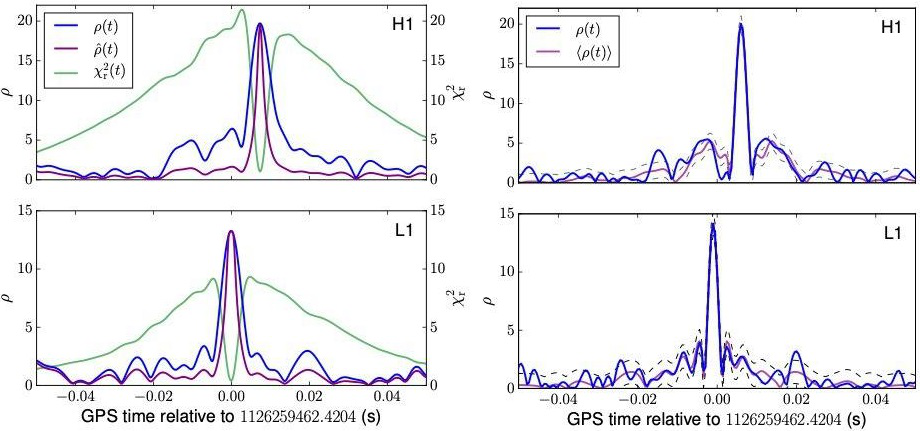
\includegraphics[scale=0.45]{firstgw}
                	\centering
                	\caption{Left: PyCBC matched-filter SNR (blue), re-weighted SNR (purple) and c2 (green) versus time of the best-matching template at the time of GW150914. The top plot shows the Hanford detector; bottom, Livingston. Right: Observed matched-filter SNR (blue) and expected matched-filter SNR (purple) versus time for the best-matching template at the time of GW150914, as reported by the GstLAL analysis. The expected matched-filter SNR is based on the autocorrelation of the best-matching template. The dashed black lines indicate 1s deviations expected in Gaussian noise.\cite{21}} 
                	\label{fig:firstgw}
                \end{figure}

\subsection{GW151226 22-Solar-Mass BBH Coalescence}

	The observation of a second coincident signal GW151226, also from the coalescence of two BHs, 
	was observed by the twin LIGO detectors, with a combined matched-filter SNR of 13. 
	The signal was identified as the second most significant event in both the PyCBC and GstLAL analyses 
	with a reweighed SNR of 12.8 and a log likelihood of 22.6, respectively. 
	GW151226 was more significant than all background events in the PyCBC analysis, 
	after having removed any background events associated with GW150914 from the distribution. \\
	Its significance assessed by its FAR is limited to be less than $6.0 \times 10^{-7} yr^{-1}$. 
	This corresponds to a p-value of $7.5 \times 10^{-8}$, or a significance of $5.3\sigma$. 
	In the GstLAL analysis, the background extends past the observed log likelihood of GW151226, 
	and the event is recovered with a FAR of 1 per 44000 years, which corresponds to a p-value of $3.5\times 10^{-6}$ and a significance of $4.5\sigma$. \\ 
	\textbf{Source Parameters}
	GW151226 persisted in the LIGO frequency band for approximately 1 s, 
	increasing in frequency and amplitude over about 55 cycles from 35 to 450 Hz, 
	this is different from the more massive GW150914 binary for which only the last 10 cycles, 
	comprising inspiral and merger, dominated the SNR. 
	As a consequence, the parameters characterizing GW151226 have different precision than those of GW150914. \\
	The chirp mass  \cite{126, 127}, which controls the binary’s evolution during the early inspiral, is determined very precisely. 
	The individual masses, which rely on information from the late inspiral and merger, are measured far less precisely. 
	The least massive BH is the secondary of GW151226, which has a 90\% credible lower bound that $m^{source}_2 \geq 5.6M_\odot$.
	This is above the expected maximum NS mass of $\sim3M_\odot$ \cite{121, 122} 
	and beyond the mass gap where there is currently a dearth of BHs observed in X-ray binaries \cite{123, 125}. 
	GW151226, corresponds to the least massive BBH system observed during O1 ($M^{source} = 21.8^{+5.9}_{-1.7}M_\odot$). \\
	The initial binary was an unequal-mass system, composed of two stellar-mass BH 
	with a source-frame primary mass $m_1. = 14.2^{+8.3}_{-2.3}M_\odot$ and secondary mass $m_2 = 7.5^{+2.3}_{-2.4}M_\odot$.
	The inferred BH masses are within the range of dynamically measured masses of BHs found in X-ray binaries \cite{128-132}, unlike GW150914. 
	Since the mass ratio for this systems is greater than GW150914,
	there is significantly greater uncertainty for the spin of the secondary than for the primary. \\
	The CBC luminosity distance can be extracted from the amplitude of an observed signal provided the orientation of the orbital plane can be determined. 
	Information about whether the orbit is face-on, edge-on, or in between is encoded in the two polarizations of the gravitational wave. 
	However, the two LIGO detectors are nearly coaligned and the source of GW151226 is likely to be located close to the maxima of the directional responses of both detectors \cite{28}. 
	Consequently, it is difficult to extract the polarization content, and therefore the orientation of the orbital plane. 
	As a result, the luminosity distance is only weakly constrained to be $D_L = 440^{+180}_{-190}Mpc$, comparable to GW150914’s, and corresponding to a redshift of $0.09^{+0.03}_{-0.04}$.
		
\subsection{GW151012 revaluated BBH}
	
	The third most significant GW event from O1, previously referred to as LVT151012,
	was detected with a low statistical significance of $1.7\sigma$, 
	corresponding to a false alarm rate of once in 2.7 years. 
	The trigger had an SNR of 9.7, therefore it was initially classified as a LIGO/Virgo Transient, 
	possibly associated with an astrophysical event. \\
	However, a detailed re-analysis of this event has demonstrated that it does indeed 
	meet the criteria of a confident detection of a BBH merger, and it is now re-labeled as GW151012.
                \begin{figure}[H]
                        \label{o1}
                        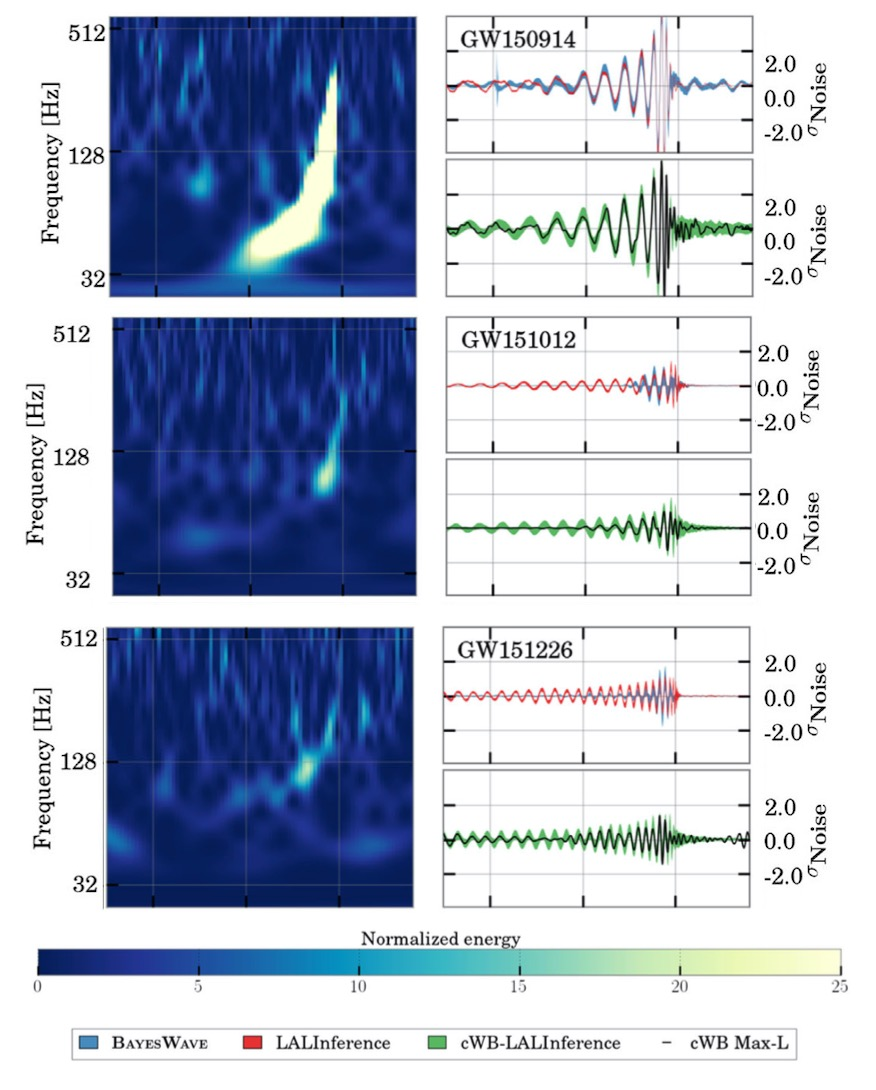
\includegraphics[scale=0.45]{o1}
                        \centering
                        \caption{Time-frequency maps and reconstructed signal waveforms for the O1 BBH events. Each event is represented with three panels showing whitened data from the LIGO detector where the higher SNR is recorded. The first panel shows a normalized time-frequency power map of the GW strain. The remaining pair of panels shows time-domain reconstructions of the whitened signal, in units of the standard deviation of the noise. The upper panels show the 90\% credible intervals from the posterior probability density functions of the waveform time series, inferred using CBC waveform templates from Bayesian inference (LALINFERENCE with the PhenomP model (red band) and by the BAYESWAVE wavelet model (blue band) The lower panels show the point estimates from the cWB search (solid lines), along with a 90\% confidence interval (green band) derived from cWB analyses of simulated waveforms from the LALINFERENCE CBC parameter estimation injected into data near each event. \cite{193}}
                         \label{fig:o1}
                \end{figure}


\section{O2: second observing run}

	After an upgrade and commissioning period, the second observing run (O2) took place from November 30, 2016 to August 25, 2017. 
	During O2, on the 1st August 2017, Advanced Virgo (AdV) joined the two aLIGO detectors for the first time, 
	taking sensitive data about 80\% of the time \cite{13}.  \\
	Between O1 and O2 run the sensitivity of both LIGO instruments was improved and 
	at LLO further improvements were made during O2. 
	As a result, the LLO BNS range increased from about 60 Mpc during O1, 
	to 80 Mpc at the beginning of O2 and then it was increased 
	by an average of about $20\%$ over all of O2. 
 	Despite the lower BNS range, during O2 was about 25 Mpc, 
	and cumulative time-volume for Virgo, its contribution has been important 
	for astrophysical parameter estimation, especially in determining source localization and orientation \cite{56}. \\
	In addition to the instruments upgrade, development were made also
	in the algorithms that search for GW signal in the observed data motivated the reanalysis of data from O1, 
	in order to reevaluate the significance of previously identified GW events and to potentially discover new ones. 
	Data from the O2 run was also reanalysed after the application of a data cleaning procedure, 
	to remove some of the detector noise and improve the sensitivity. \\
	Of the eight GW signals detected during O2, five were localized by the three detector LHO, LLO and Virgo (HLV) network. 
	Consequently, the detection accuracy is  due to the addition of AdV to the network. 
	The second observing run is divided into periods of two-detector cumulative 
	coincident observing time with 5 days of data to measure the false alarm rate 
	of the search at the level where detections can be confidently claimed. 
	The searches can target BBH mergers with detector-frame total masses $2M_\odot \leq M^{det} \leq 500 M_\odot$,
	and spin magnitudes up to $\sim0.99$.
	The upper mass boundary of the bank is determined by imposing a lower limit on the duration of the template in the detectors’ sensitive frequency band.



\subsection{GW170104 50-Solar-Mass BBH Coalescence}

	The observation of GW170104 was made by LIGO detectors, 
	with a network SNR of 13 and a false alarm rate less than 1 in 70,000 years.
	At the detection statistic value of GW170104, the background rate in both matched filter 
	analyses is dwarfed by the signal rate, yielding a $P_{astro} > 1 - (3 \times 10^{-5)}$. \\
	GW170104’s source is a heavy BBH system, with a total mass of $\sim50M_\odot$,	
	the inferred component BH masses are $31.2^{+8.4}_{-6.0}M_\odot$ and $19.4^{+5.3} _{-5.9}M_\odot$ (at the 90\% credible level). 
	The BH spins are best constrained through measurement of the effective inspiral spin parameter, $\chi_{eff}$, 
	a mass-weighted combination of the spin components perpendicular to the orbital plane, $\chi_{eff} = −0.12^{+0.21}_{−0.30}$. 
	This result implies that the BH spins show a preference away from being 
	(positively) aligned with the orbital angular momentum, but do not exclude zero spins. 
	This is distinct from the case for GW151226, which had a strong preference 
	for spins with positive projections along the orbital angular momentum \cite{58}. \\
	The source luminosity distance is $880^{+450}_{−390} Mpc$ corresponding to a redshift of $z = 0.18^{+0.08}_{−0.07}$. 
	Stars losee mass throughout their lives; to leave a heavy BH as a remnant 
	they must avoid significant mass loss. 
	Low-metallicity progenitors are believed to have weaker stellar winds and hence diminished mass loss \cite{135}. 
	The heaviness of the source masses suggests formation in a sub-solar metallicity environment \cite{134}. 
	The inferred merger rate agrees with previous calculations \cite{59, 137}, and could potentially be explained 	
	by BBHs forming through isolated binary evolution or dynamical interactions in dense stellar clusters \cite{134}. 

\subsection{GW170608 19 Solar-mass BBH Coalescence}

	GW170608 was first identified as a loud (SNR $\sim9$) event in LLO data,
	via low-latency templated searches \cite{138}.	
	The morphology of the LLO event is consistent with a compact binary merger signal, 
	but a noise origin could not be ruled out using LLO data alone. 
	Consequently, LHO data were investigated and were determined to be stable 
	at frequencies above 30Hz, which was established as the starting frequecy to look into a segment of LHO data around the event time.
	Two matched filter pipelines identified GW170608, with a network SNR of 13 
	and a rate of occurrence of noise events of less than 1 in 3,000 years for the PyCBC pipeline, 
	and a false alarm rate of 1 in 160,000 years for GstLAL. \\
	The binary of GW170608 consisted of two compact objects with source-frame component masses 
	$m_1 =12^{+7}_{-2}M_\odot$ and $m =7^{+2}_{-2}M_\odot$.  
	Since NSs are expected to have masses below $\sim 4M_\odot$ \cite{141},
	both objects are most likely BHs. 
	The $\chi_{eff}$ inferred from this event is $0.07^{+0.23}_{−0.09}$,
	disfavoring large, anti-aligned spins on both BH. \\
	GW170608 is localized at a luminosity distance of  $D_L = 340^{+140}_{−140}Mpc$, and to a sky area of $\sim520 deg^2$, determined largely by the signal’s measured arrival time at LLO $\sim7$ ms later than at LHO. 
	The low mass of GW170608’s source binary, in comparison to other BBH systems 
	observed by LIGO and Virgo, has potential implications for the binary’s progenitor environment. 
	High-metallicity progenitors are expected to experience substantial mass loss through strong stellar winds \cite{142}.
	GW170608’s low mass suggests formation in a higher metallicity environment; 
	however, formation at lower metallicity with comparatively lower mass progenitors is not excluded. 
	At this lower boundary of the observed distribution of BBH masses, 
	a comparison between the component BHs with those found in X-ray binaries is possible.
	X-ray binary systems contain either a BH or NS which accretes matter from a companion donor star. 
	The inferred component masses of GW170608 are consistent with dynamically-measured masses of BHs found in low-mass X-ray binaries.

\subsection{GW170814 Three-detector Observation of BBH Coalescence}	
	
	On August 14, 2017, a GW signal coming from the merger of two stellar mass BH 
	was observed for the first time by a three detector network, with the Virgo and LIGO detectors. 
	GW170814 was first identified with high confidence by two independent 
	low-latency matched-filter pipelines \cite{111,143-146,149},
	with a Hanford-Livingston network SNR of 15 and a three-detector network SNR of 18. \\
	Ranking statistic values from the two pipelines correspond to 
	a false-alarm rate of 1 in 140 000 years in one search \cite{114,143} 
	and 1 in 27 000 years in the other search \cite{111,146,149,150}, 
	clearly identifying GW170814 as a GW signal. 
	These results did not use data from Virgo for significance estimates.
	The significance of GW170814 was confirmed by 
	an independent coherent analysis that targets 
	generic GW transients with increasing frequency over time \cite{151},
	which includes Virgo data. 
	The improved significance achieved by adding the data from Virgo 
	can be shown by comparing the results of this analysis with 
	all the detectors with the results with only LIGO data.
	The former case reports a false-alarm rate < 1 in 5900 years,
	while the latter the false-alarm rate is approximately 1 in 300 years. \\ 
	The parameters of the source inferred through a coherent Bayesian analysis \cite{93, 152} 
	of offline noise-subtracted data for the LIGO and Virgo detectors, 
	%the absence of precession \cite{154-160}, 
	%dynamics through a rotation of an originally nonprecessing model \cite{161,163,164}. 
	are the  masses of the initial black BH, $30.5^{+5.7}_{-3.0}M_\odot$ 
	and $25.3^{+2.8}_{-4.2}M_\odot$, at the 90\% credible level. \\
	Before the addition of Virgo, the localisation of most mergers 
	was restricted to roughly annular regions by the baseline formed by the two LIGO detectors,
	spanning hundreds to about a thousand square degrees at the 90\% credible level \cite{165-167}. 
	The inclusion of Virgo contributes with additional independent baselines, 
	which in cases such as GW170814 can reduce the positional uncertainty by an order of magnitude or more \cite{166}. 
	With a network of detectors, sky position can be inferred by triangulation employing 	
	the time differences \cite{168,169}, phase differences, and amplitude ratios on arrival at the sites \cite{170}. 
	For an initial rapid localization from Hanford and Livingston, 
	the 90\% credible area on the sky is $1160 deg^2$ and shrinks to $100 deg^2$ when including Virgo data. 
	Incorporating Virgo data also reduces the luminosity distance uncertainty from 
	$570^{+300}_{-200}Mpc$ (rapid localization) to $540^{+130}_{-210} Mpc$ (full parameter estimation). \\
	 Since the two LIGO instruments have similar orientations, little information about polarizations 
	can be obtained using the LIGO detectors alone, therefore including Virgo in the search 
	allows for the first time to investigate GW polarizations, by geometrically 
	projecting the wave’s amplitude onto the three detectors. \\
	Generic metric theories predict that any combination of tensor, vector, or scalar 
	polarizations \cite{171,172} characterize metric perturbations.
	So far, some evidence that GWs are described by the tensor (spin-2) metric perturbations 
	of general relativity has been obtained from measurements of the rate of orbital decay of binary pulsars \cite{173,176}, 
	and from the rapidly changing GW phase of BBH mergers observed by LIGO, in the framework of parametrized models \cite{52,57,60}. 
	The results from this analysis show that the data strongly favor
	pure tensor polarization of GWs, over pure scalar or pure vector polarizations. \\
	The black hole characteristics of GW170814 are similar to GW150914 and GW170104, 
	and are found to be consistent with the astrophysical population and merger rate determined with previous detections.
		\begin{figure}[H]
                        \label{o2}
                        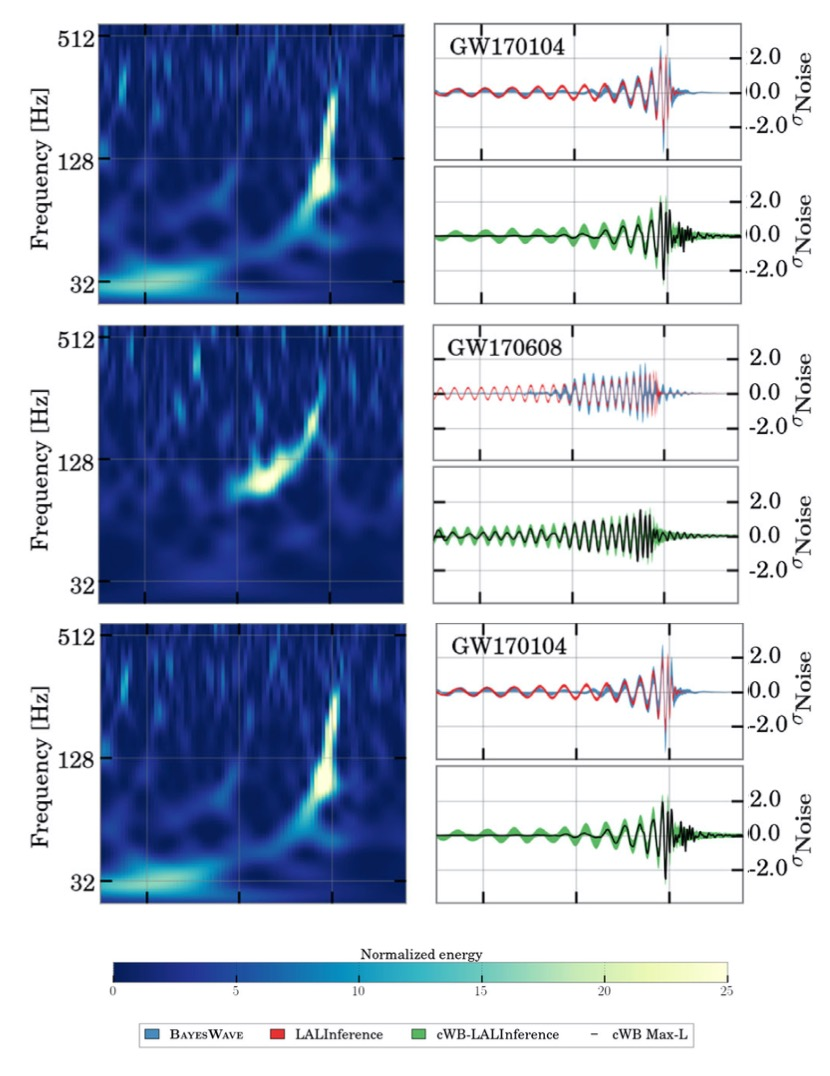
\includegraphics[scale=0.45]{o2}
                        \centering
                        \caption{Time-frequency maps and reconstructed signal waveforms for some of the O2 BBH event Each event is represented with three panels showing whitened data from the LIGO detector where the higher SNR is recorded. The first panel shows a normalized time-frequency power map of the GW strain. The remaining pair of panels shows time-domain reconstructions of the whitened signal in units of the standard deviation of the noise. The upper panels show the 90\% credible intervals from the posterior probability density functions of the waveform time series, inferred using CBC waveform templates from Bayesian inference (LALINFERENCE) with the PhenomP model (red band) and by the BAYESWAVE wavelet model (blue band). The lower panels show the point estimates from the cWB search (solid lines) along with a 90\% confidence interval (green band) derived from cWB analyses of simulated waveforms from the LALINFERENCE CBC parameter estimation injected into data near each event.}
                         \label{fig:o2}
                \end{figure}


\subsection{Gamma Ray Burst}

	Discovered fortuitously by the Vela satellites in the late 1960s \cite{180}, 
	gamma-ray bursts (GRBs) are brief, $\Delta t \sim 0.1-100s$, intense, flashes of high-energy, 1 keV–10 MeV, radiation 
	produced when an ultra-relativistic fireball of high energy photons is launched from some central engine. 
	In most cosmological scenarios, as well as a few galactic ones, 
	the large energy density at the source implies that the plasma produced 
	undergoes relativistic expansion \cite{181}.
	An important consequence of this scenario, as well as the prompt emission of gamma-ray emission from internal shocks, 
	is the prediction that this fireball will produce detectable afterglow emission in the X-ray and sometimes optical and radio bands \cite{182},	
	after ploughing into the external medium, surrounding the source \cite{153,162}. \\ 
	Collected data from the Swift and Fermi satellites show 
	that the observed spectra are composed of several distinctive components:
	the spectra of both the prompt and afterglow emission is non-thermal, 
	the prompt emission also has an exponential high energy cutoff.
	Broadband simultaneous spectral energy distributions  
	reveal the presence of spectral breaks, showing that the spectrum is composed of multiple, 
	smoothly connected power law branches. 
	The spectral break frequencies are seen to evolve during time, 
	and the peak of the spectrum to move towards lower frequencies. 
	There are evidence that the very high energy part of the spectra evolve differently than the lower energy part, 
	hence is likely to have a separate origin. 
	The sharp cutoff in the lightcurves of many GRBs observed by Swift enables a clear discrimination between the prompt and the afterglow phases.  \\
	The afterglow is believed to be synchrotron emission caused by the shocked external medium: after producing the prompt emission, the GRB ejecta move at relativistic speed 
	and they expand into the interstellar medium, sweeping it. 	
	As soon as the rest mass of the collected interstellar medium becomes comparable 
	to the kinetic energy of the ejecta, a strong shock wave is formed. 	
	At the shock, electrons are accelerated by the Fermi process and radiate mainly by synchrotron emission\cite{153,162}. 
	In many cases, the decay of the optical or X-ray afterglow light-curve steepens 
	to $F_{\nu} \propto t^{−2.2}$ at $\sim 1$ day after the burst, meaning that GRB outflows 
	are not spherical but collimated into narrow jets \cite{183}. 
	As the ejecta is decelerated and the strength of the relativistic beaming diminishes, 
	the edge of the jet becomes visible to the observer. 
	Distances to GRBs were completely uncertain until the launch of Compton-Gamma-Ray-Observatory (CGRO),  	
	which discovered roughly one new GRB per day and established that these bursts 
	are isotropically distributed, meaning they occur everywhere in the cosmos \cite{184}.\\
	Burst redshift and flux show that GRBs radiate between $10^48$ and $10^55 ergs$, if isotropic.
	This means that they are the most powerful outbursts of electromagnetic (EM) radiation in our universe 
	and a possible source of (ultra) high-energy cosmic rays \cite{185,186}. 
	After the discovery of the afterglow, a distinction between the initial gamma-rays 
	and the subsequent longer wavelength counterpart became necessary: 
	observationally, the prompt emission phase of a GRB is conventionally defined 
	as the temporal phase during which sub-MeV emission is detected by 
	the GRB triggering detectors above the background level. \\
	Quantitatively, the duration of a burst is defined by the so-called $T_90$: 
	the time interval between the epochs when 5\% and 95\% of the total fluence is registered by the detector. 
	Fluence here is the gamma-ray flux received in the detector integrated over the duration of the GRB. \\
	The histogram of GRB duration has two distinct peaks:
	one at $0.3s$ and the other at about $30s$, and there is a trough in between the peaks at $2s$. \\
	Bursts with duration less than $2s$ are classified as short-GRBs (SGRB) 
	and those that last for more than $2s$ are called long-GRBs.
	The two peaks in the duration distribution indicate the existence of 
	two progenitor source classes: mergers of compact object
	and rapidly spinning, hydrogen-stripped massive stars. 
	These models are linked with SGRBs and LGRBs respectively. 
	The secure association of SGRB with with both elliptical and star-forming galaxies
	demonstrates unambiguously that some of the GRB progenitors are related to an old stellar population. 
	Moreover, an analysis of the distribution of SGRB offsets relative to their 
	host galaxy centers indicated that SGRB progenitors are compact object binaries. 
	These observation led to the association of SGRB with mergers of NS 
	with other NS or with BH, which was confirmed with the joint observation of GW170817 and GRB170817A. \\
	The Fermi Gamma-ray Space Telescope is currently the most efficient GRB detection satellite in orbit. 
	Its two main instruments are the Large Area Telescope (LAT) and the Gamma-ray Burst Monitor (GBM). 
	Whereas LAT has a sky coverage of 20\%, GBM continuously observes the full region of the sky not occulted by Earth. \\ 
	The Swift satellite is a first-of-its-kind multi-wavelength observatory:
	it has X-ray and UV-optical telescopes on board and provides localization of bursts to within 3 arcminutes. 
	When Swift’s gamma-ray telescope (Burst and Altert Telescope or BAT) detects a burst, 
	the X-Ray Telescope (XRT) and the UV-Optical Telescope (UVOT) on board Swift quickly slew to the 
	GRB position within 60-100 seconds to observe the target, which provides excellent coverage 
	of the transition from the prompt gamma-ray phase to the lower-frequency afterglow emission phase.

\subsection{GW170817: first BNS detection}

	On 2017 August 17 the first confident joint EM–GW observation in history was made when 
	a coincident GW trigger by LIGO occurred $\sim1.7s$ prior to the announcement of a GBM trigger \cite{147},
	which was later designated GRB170817A \cite{140}.
	The comparison of the Fermi-GBM Gamma-ray Coordinates Network (GCN) notice to the GW 
	trigger shows the small time offset between the events which, together with an independent localization of the triggers,
	allowed an unambiguous association of these two events. 
	The GW170817 candidate was registered in low latency \cite{112,114}
	based on a single-detector analysis LHO data. 
	Rapid offline re-analysis \cite{28,111} of data from the LIGO/Virgo network 
	confirmed the presence of a significant coincident signal in the LIGO GW detectors with a combined SNR of 32.4. \\
	The offline analysis then identified GW170817 with a false-alarm rate of less than 1 in 80,000 years \cite{61}. 
	A coherent Bayesian analysis \cite{59,152}
	inferred the GW source localisation in a region of $28 deg^2$ at a distance of $40^{+8}_{-14}$ Mpc, 
	consistent with the early estimates disseminated through GCN Circulars \cite{55,60}. \\ 
	The inspiral phase of the binary coalescence dominates 
	the portion of GW170817 in the instruments’ sensitivity band, 
	and as a consequence, the chirp mass, which drives the frequency evolution of gravitational radiation at the leading order, 
	is the best constrained parameter with a value of $1.188^{+0.004}_{-0.002}M_\odot$.
	The measured component masses are in the range 0.86 to 2.26 $M_\odot$
	consistent with a binary whose components are neutron stars. \\
	Two offline targeted coherent searches were employed to analyse the LIGO-Virgo data: 
	the first targeted search \cite{111,116,213}
	assumes that the source is a BNS or NS–BH binary merger and is located at the sky-position 
	observed for the optical counterpart to GW170817 and GRB170817A \cite{55,136}, 
	and that there is a $[-1, +5] s$ time delay in the arrival of gamma-rays (determined by the GBM trigger time) 
	compared to the binary merger time \cite{55}. 
	At the detection statistic value assigned to GW170817, this search has a p-value of $<9.4\time 10^{-6}(>4.2\sigma)$, 
	with this significance estimate limited by computational resources used to estimate the noise background. 
	The second coherent search does not assume any particular GW morphology or GRB model 
	\cite{55,144,145} and uses the GBM localization of GRB170817A 	
	to constrain the sky location of the source. This search allows for a $[-60, +600] s$ 
	coincidence between the gamma-rays and the GWs in order to include potentially 
	larger delays in collapsar models of long GRBs. 
	At the detection-statistic value observed for GW170817, this search has a p-value of $1.3\times 10^{-5} (4.2\sigma)$. \\ 
	Standard follow-up analyses \cite{108,110} of the Fermi-GBM trigger 
	determined the burst duration to be $T_{90} = 2.0 \pm 0.5 s$,
	therefore GRB 170817A was classified as a sGRB, with 3:1 odds over being a long GRB. 
	The classification of GRB170817A as an sGRB is further supported by incorporating 
	the hardness ratio of the burst and comparing it to the Fermi-GBM catalog \cite{110}. 
	The electromagnetic observations further support the interpretation of the nature of the binary, 
	and comprise three components at different wavelengths: a prompt sGRB that demonstrates 
	that BNS mergers are the progenitor of at least a fraction of such bursts; an ultraviolet, optical, 
	and infrared transient (kilonova), which allows for the identification of the host galaxy 
	and is associated with the aftermath of the BNS merger; 
	delayed X-ray and radio counterparts that provide information on the environment of the binary. 
	A major astrophysical implication of a joint detection of an SGRB and of GWs from a BNS merger 
	is the confirmation that these binaries are indeed the progenitors of at least some SGRBs. 
		\begin{figure}[H]
                        \label{gw-grb}
                        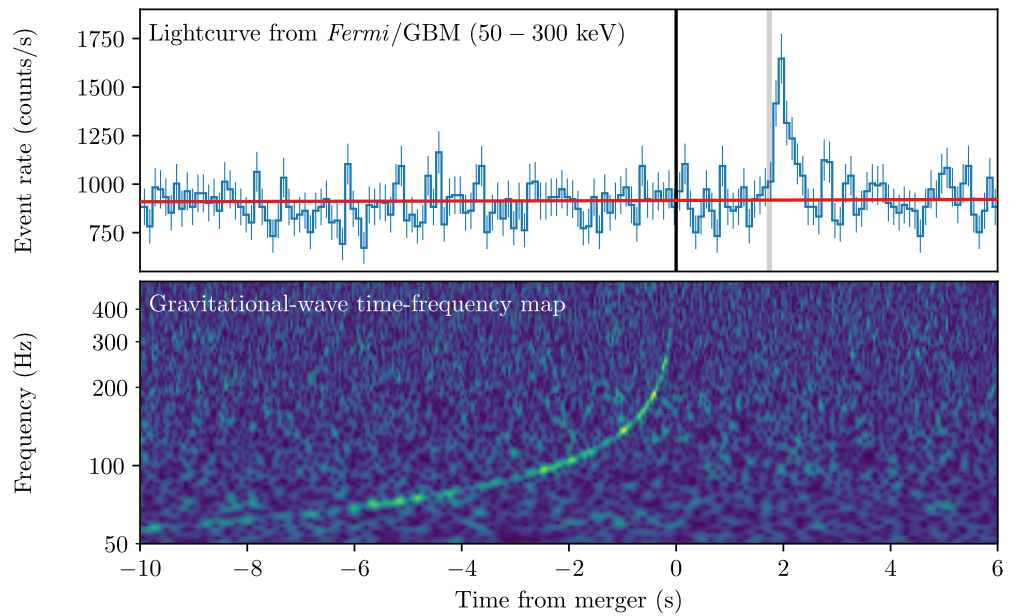
\includegraphics[scale=0.45]{gw-grb}
                        \centering
                        \caption{Joint, multi-messenger detection of GW170817 and GRB170817A. Top: the summed GBM lightcurve for sodium iodide (NaI) detector for GRB170817A in the 50–300 keV energy range matching the 100 ms time bins of the SPI-ACS data. The background estimate from \cite{110} is overlaid in red. Bottom: the time-frequency map of GW170817 was obtained by coherently combining LHO and LLO data. All times here are referenced to the GW170817 trigger time $T_0^{GW}$. \cite{55}}
                        \label{fig:gw-grb}
                \end{figure}

\section{O3a: first half of the third observing run}

	On April 1, 2019, Advanced LIGO and Advanced Virgo initiated their third observing run (O3), 
	and was prematurely suspended on March 27th 2020 \cite{53}.
	Between O2 and O3, several improvements were made to increase the detectors’ sensitivity: for the LIGO detectors, 
	the changes consisted in increasing the input laser power, adding a squeezed vacuum source 
	at the interferometer output and mitigating noise arising from scattered light .  
	Additionally, end test-mass optics with lower-loss coatings, along with new reaction masses, 
	have been installed in each interferometer \cite{53}. 
	The BNS inspiral range was $102-111 Mpc$ for LHO and $125-140 Mpc$ for LLO during the first phase of O3. \\
	 Also joining O3 was Virgo, with double the sensitivity since its last run, thanks to a series of improvements: 
	fused silica fibers were installed on the Advanced Virgo, as a replacement of the steel test-mass suspensions;
	other upgrades included reducingtechnical noises, increasing the input laser power 
	and installation of a squeezed vacuum source. 
	The Virgo BNS inspiral range was about $43–50 Mpc$ over the first three months of O3, as shown in Fig.$\ref{fig:o3bnsrange}$. 
                \begin{figure}[H]
                        \label{o3bnsrange}
                        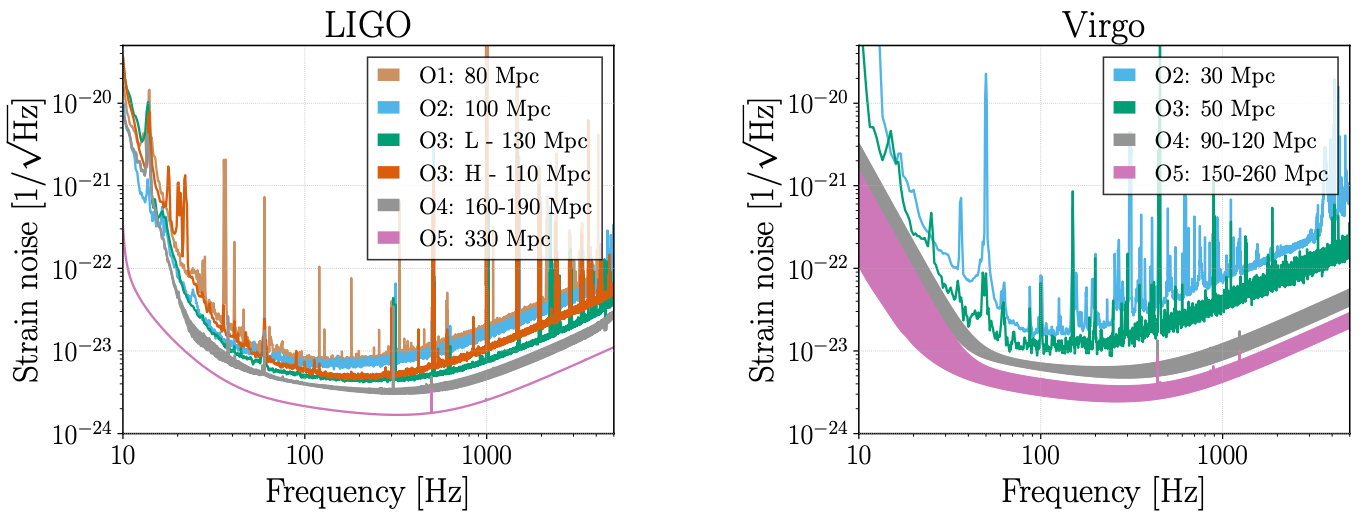
\includegraphics[scale=0.5]{o3bnsrange}
                        \centering
                        \caption{Advanced LIGO (top left), Advance Virgo (top right) target strain sensitivities as a function of frequency. The quoted range is for a [-$1.4M_\odot, 4 M_\odot]$ BNS merger. The BNS range (in megaparsec) achieved in past observing runs and anticipated for future runs is shown. The O1 aLIGO curve is taken from the LHO, the O2 aLIGO curve comes from the LLO. In each case these had the better performance for that observing run. The O3 curves for aLIGO and AdV reflect recent performance. For some runs the anticipated ranges are shown as bands reflecting the uncertainty in the impact of improvements and upgrades to the overall sensitivity. \cite{53}}
                        \label{fig:o3bnsrange}
                \end{figure}
	These improvements successfully impacted the detection: in spite of the early suspension, 
	56 detection candidates have already been announced as public alerts, Fig.$\ref{fig:o3detection}$.
                \begin{figure}[H]
                        \label{o3detection}
                        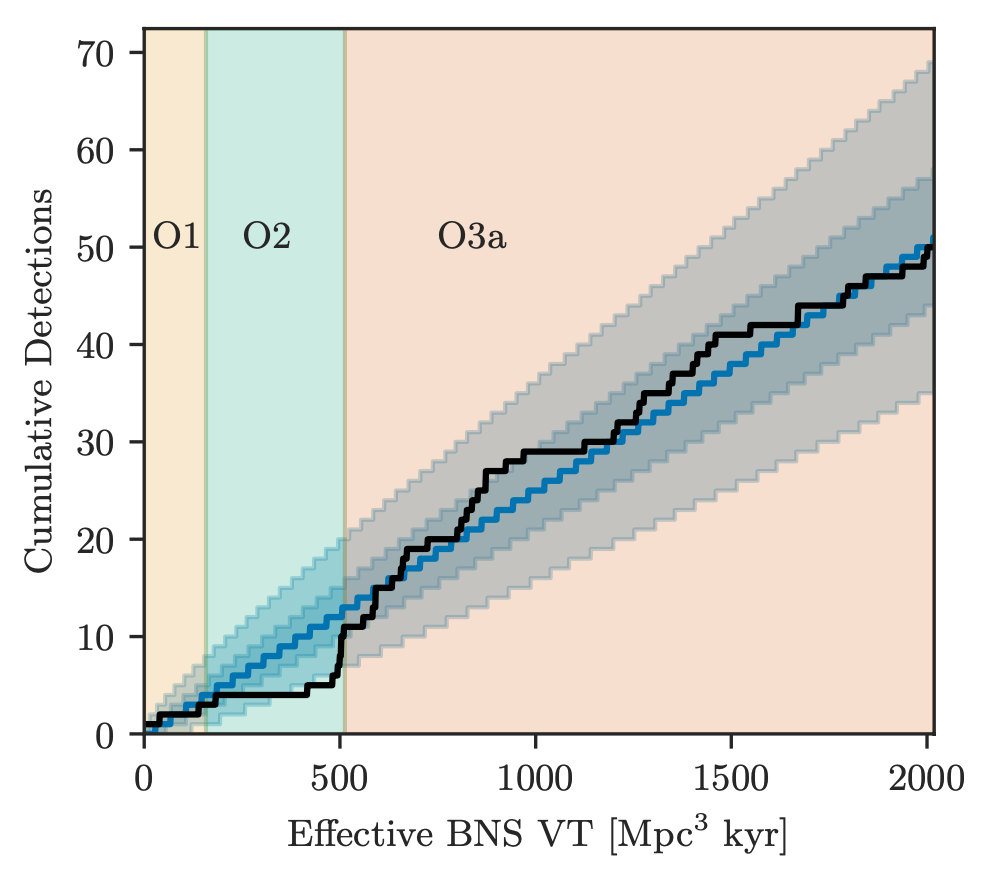
\includegraphics[scale=0.22]{o3detection}
                        \centering
                        \caption{LIGO's third observing run yielded 56 gravitational-wave detections. That's 5-times more than were collectively made during O1 and O2, that yielded 11 gravitational wave detections. Image credit: LIGO-Virgo Collaboration}. 
                        \label{fig:o3detection}
                \end{figure}

\subsection{GW190425: Observation of a compact binary coalescence with total mass ~3.4 Msun}

	On 2019 April 25, the LLO observed the second GW signal, GW190425, 
	consistent with the inspiral of a BNS system of component masses in the range from $1.12$ to $2.52 M_\odot$ 
	This event was detected in real time processing, with an SNR of 12.9 in LLO; 
	Virgo was operating at the time of the event, the SNR it observed was only 2.5, 
	which is below the threshold of 4.0 at which searches consider triggers for significance estimation. 
	The difference in SNR between LLO and Virgo is consistent with the difference 
	in the sensitivities of the two detectors, considering that LLO had 
	a BNS inspiral range of $\sim135 Mpc$, while Virgo had of $\sim48 Mpc$. \\
	The single detector observation has a couple of consequences: 
	the area on the sky that would constrain this event is large which 	
	makes a significant challenge for follow-up searches for EM counterparts. 
	No EM counterpart means that there is no confirmation that this was a BNS; 
	it’s therefore possible that one or both of the merging objects was actually 
	a BH smaller than any BH detected so far \cite{148}.
	In addition, having an event in a single GW detector means that there are not other 
	observatories data to check for signal consistency against. 
	The low-latency FAR as estimated using the data collected in O3 
	up until the time of the event, and it was found to be one in $69,000 yr$. 
	To further establish the significance of GW190425, it was compared against the 169.5 
	days of background from O1 and O2 and 50 days of background 
	from O3 in the BNS part of the parameter space, and found to be 
	louder than any background event \cite{148}. \\
	The binary heaviest component mass is between $1.61M_\odot$ and $2.52 M_\odot$, 
	while the mass of the second object between $1.12M_\odot$ and $1.68 M_\odot$.
	This event is particularly special because of its total mass of $3.4^{+0.3}_{-0.1} M_\odot$ 
	and chirp mass of $1.44^{+0.02}_{-0.02}M_\odot$, which are are significantly larger 
	than those of any other known Galactic BNS system. 
	Currently, there are 17 known galactic neutron star pairs with measured total masses 
	that range from $2.5$ to $2.9 M_\odot$. 
	Fitting a normal distribution to the total masses of ten galactic BNS systems, 
	which are expected to merge within the lifetime of the Universe, 
	shows that the average galactic binary mass is about $2.69 M_\odot$, 
	while the mass of the GW190425 binary is about $3.4 M_\odot$, 
	lying 5 standard deviations away from the Galactic mean, as shown in Fig$\ref{fig:secondbns}$. \\ 
	GW190425’s unusual mass may have implications for the system’s origin \cite{148}.
	There are two ways in which we expect to form a binary with two neutron stars. 
	Massive, fast-merging neutron-star pairs could potentially result from 
	especially low-metallicity stars evolving in close binary systems, undergoing a supernova explosion.
	If this is the case, GW190425 could represent a population of BNS never observed before, 
	because ultra-tight orbits NS systems with sub-hour periods are not detectable by current EM surveys.
	Another formation channel is the dynamical one: a third NS joins an already existing binary, 
	which could be a BNS or a NS with a main sequence star, kicking out the
	lower mass star and leaving behind a binary containing two NS.
	The inferred NS’s spins are also consistent with the spins of the two fastest 
	spinning Galactic BNS that are expected to merge within the lifetime of the Universe. \\
	In the BNS scenario, the detection of GW190425 provides an update 
	on the number of NS that collide in a volume of the universe every year of $250–2810 Gpc^{-3}yr^{-1}$ \cite{62}.
		\begin{figure}[H]
                        \label{secondbns}
                        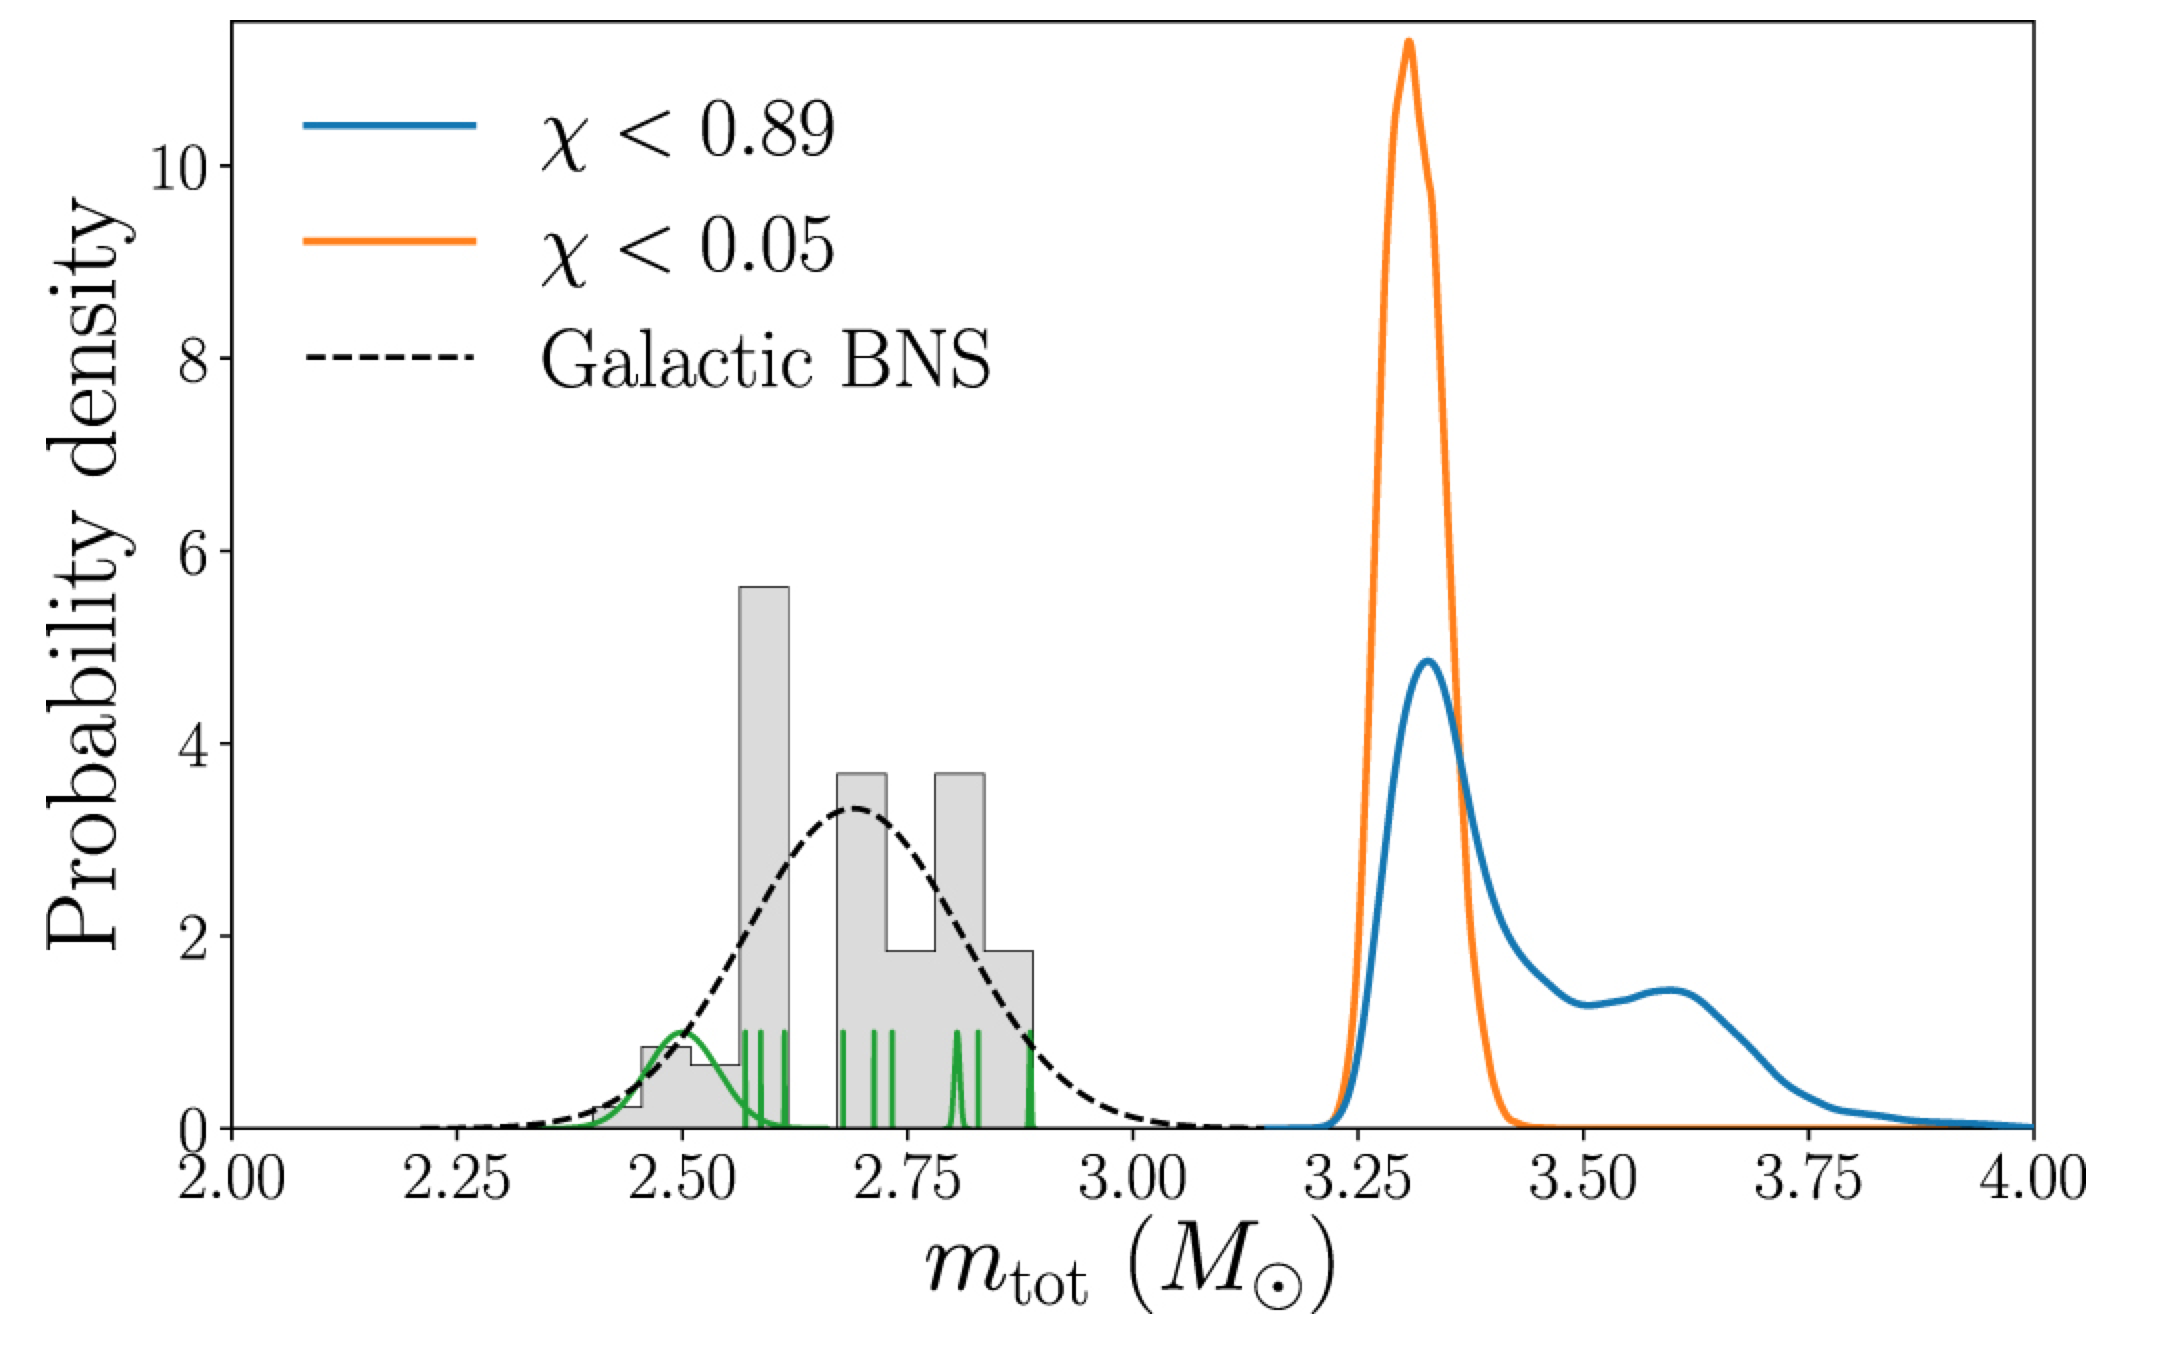
\includegraphics[scale=0.3]{secondbns}
                        \centering
                        \caption{Blue and orange curves show the estimated total mass of GW190425 under different spin assumptions. In either case, the estimated mass is dramatically different from the total masses for the known galactic population of BNS, indicated with the grey histogram bars and the dashed line. \cite{62}}
		        \label{fig:secondbns}
                \end{figure}


\subsection{GW190412: Observation of a Binary-Black-Hole Coalescence with Asymmetric Masses}

	GW190412 is a loud event detected with a three detector network SNR of 19 and a FAR of 1 over 30000 yr.
	The peculiarity of this event is the asymmetry in the binary component masses:
	one BH was $\sim8 M_\odot$, while the other companion $\sim30 M_\odot$.
	While the individual masses of the BBH were consistent with what has been observed in
	prior observing runs, the mass ratio is unlike any of the other BH mergers detected before. 
	Therefore, the GW frequency from each of the BH’s orbit was different: 
	the heaviest was likely producing a lower frequency, while the lighter one was producing a higher frequency.
	This inequality allows to observe a fundamental property of GWs. \\
	Gravitational radiation from CBC was shown to be predominantly quadrupolar \cite{177-179} 
	and is observed as a combination of two polarizations, weighted with the detector response functions, see Eq.$\ref{beampattern}$. 
	This quantity can be expressed also as $h = h_{+}-ih_{\times}$ and expanded into multipole moments 
	using spherical polar coordinates defined in a source centered frame \cite{225}
		\begin{equation}
			h_{+}-ih_{\times} = \sum_{l \geq 2} \sum_{-l \leq m \leq l} {{h_{lm}(t, \boldsymbol{\lambda})} \over {D_L}} _{-2} Y_{lm}(\theta, \phi)
		\end{equation}
	The radiative multipoles, $h_{lm}$, depend on source properties, while the source geometry 
	depends on mass ratio and is most prominently manifested in the relative contribution 
	of multipoles with odd or even azimuthal index, $m$.
	For an exactly equal mass binary with non-spinning components, only multipoles with even $m$ 
	respect orbital symmetry and so are present in the radiation \cite{187}, resulting in the quadrupole, $h_{22}$, 
	to be the most dominant, followed by other multipoles with even $m$. 
	Otherwise, for sufficiently unequal mass ratios, the $l = m = 3$ and subsequent 
	multipoles with $l = m$ gain increasing importance \cite{187-192}. \\
	GWs of higher harmonics had not been observed until GW190412:
	these higher multipoles makes a significant, measurable contribution to the observed data as shown in \cite{133}. \\
	As a result, the orientation of the binary is more accurately determined and 
	tighter bounds are obtained on relevant intrinsic source parameters such as the mass ratio and primary spin magnitude, 
	which is the strongest constraint on the individual spin magnitude of a BH using GWs so far. 
	Even though the $\chi_{eff}$ is found to be positive, there are not lare in-plane spin component, 
	hinting that the system is slightly precessing.
	The degeneracy between luminosity distance and inclination angle that is present 
	in the results obtained without higher multipoles, is broken when higher multipoles are included, 
	resulting in more precise measurements of these parameters. \\ 
	The new observation also provides new insight into the merging BBH rate, 
	and how clearly unequal-mass system are less unlikely but still expected to form in the universe. \cite{133}
                \begin{figure}[H]
                        \label{asymmetric}
                        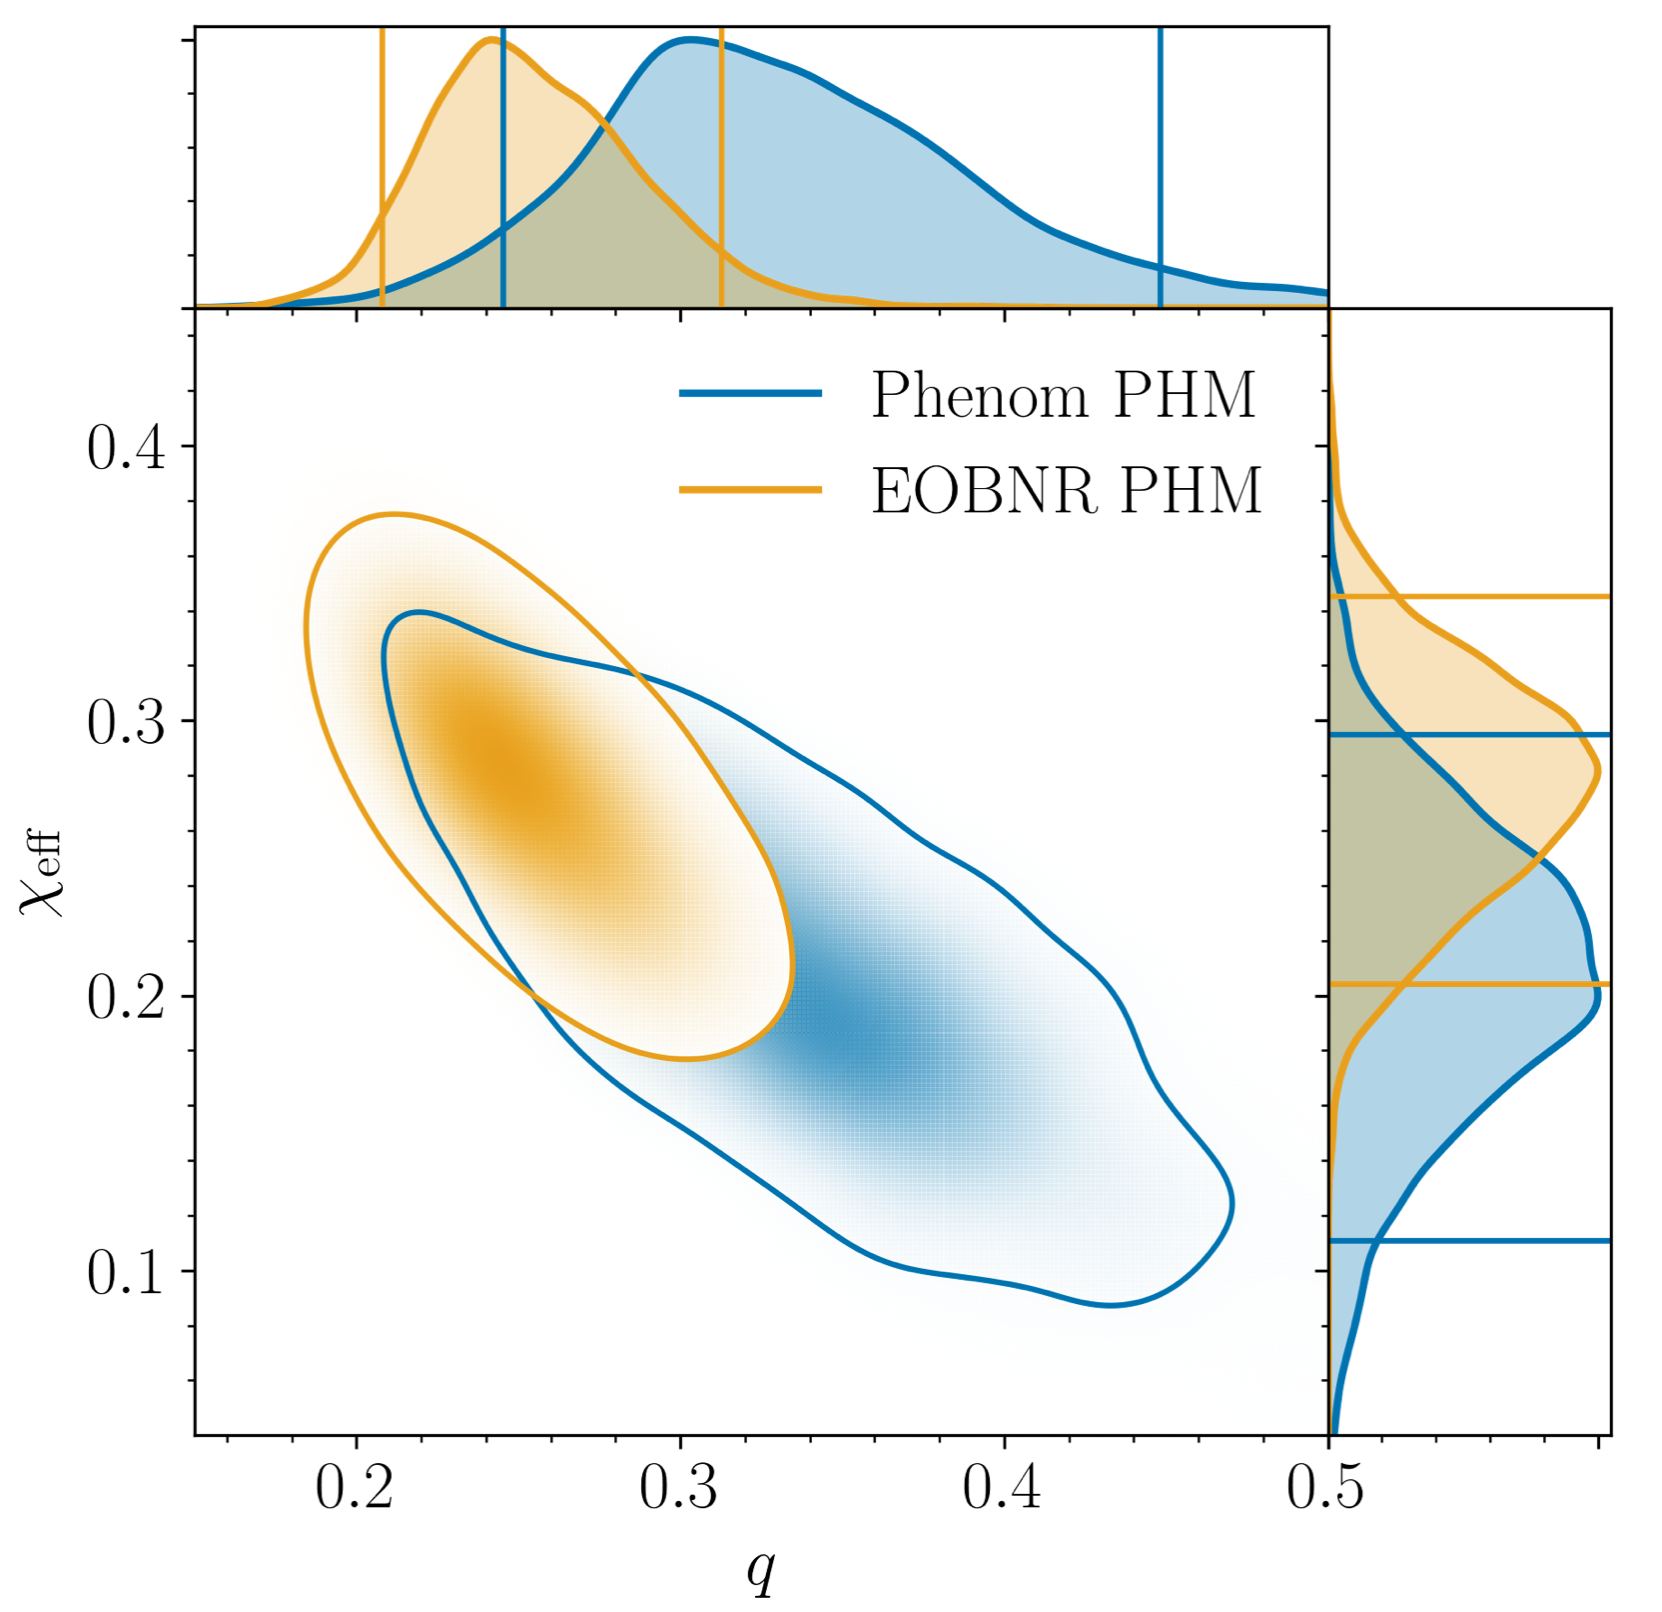
\includegraphics[scale=0.2]{asymmetric}
                        \centering
                        \caption{The inferred mass ratio $q$ and effective spin $\chi_{eff}$ of GW190412. The orange and blue contours show the distributions on the parameters recovered using two different waveform models, which make slightly different approximations for modeling the true general-relativistic signal.\cite{133}} 
                        \label{fig:asymmetric}
                \end{figure}

%----------------------------------------------------------------------------------------------------------------------------------------------------------------------------------------------------------

\chapter{Black hole-neutron star binaries}

        Black holes and neutron stars are the densest object in the universe resulting from gravitational collapse,
        and extraordinary cosmic laboratories to probe gravity in the strong-field regime.
        BHs represent the extremes of space-time curvature:
        they have no surface, just an event horizon which separates the information
        from within the BH’s interior from the outside universe;
        they are the most simple fundamental objects in the universe
        as they are entirely described by two parameters, mass and spin.
        On the other hand, NS represent both the extremes of space-time as well as dense matter.
        Both NSs and BHs represent the end states of the lives of massive stars
        and their masses essentially range from one to a few solar masses,
        crammed into objects with radii of ten to fifteen kilometers. \\
        Informations on the properties of BH and NS in NSBH binaries come from
        their observation in other types of binary systems or from theoretical considerations:
        while most NS observed in BNS systems have masses in the [1.2 − 1.6] $M_{\odot}$ range %\cite{}, 
        more massive NS exist, up to at least $\sim$ 2$M_{\odot}$  %\cite{}. 
        Most galactic BH have masses of [5 − 15] $M_{\odot}$  %\cite{}, 
        but BHs observed through GWs are often more massive %\cite{}. \\ 
        NSBH binaries are believed to form both in isolated binaries,
        and through dynamical interactions in star clusters, nuclear clusters and galactic nuclei \cite{194}.
        Large number of BHs and NSs and the presence of heavy BHs can impact significantly
        the probability for NSBH binary to form and, possibly, merge. \\
        Whether BHs can be formed within the “mass gap” between the most massive NS
        and $\sim$ 5$M_{\odot}$ also remains an important open question. \\
        The magnitude and orientation of BH spins are unknown, and while most NSBH binaries
        are expected to have negligible eccentricities %\cite{}, 
        eccentric NSBH binaries cannot entirely be ruled out
        and have evolutions very distinct from circular binaries %\cite{}. \\
        The evolution of the BH singularity and the presence of matter combine
        the difficulties of evolving both BBHs and BNS, and the system has its own specific challenges,
        specifically the accretion of the NS matter onto the BH.
        Such binaries are not only sources of GW radiation, but also potential sources of GRBs.
        Since the first GW detection, the GW catalog has expanded collecting GW signals from BBH and BNS.
        However, gravitational proof of the NSBH interaction is yet to be achieved:
        this event would display a much richer phenomenology than BBH mergers,
        even in the relatively simple case of both non-spinning objects.
        From this last missing detection we are able to extract and learn about
        the sources fundamental properties, such as the BH’s masses and spins
        as well as the NS equation of state (EOS), because the orbital frequency at tidal disruption
        depends strongly on the compactness of the NS, $C_{NS}$ (Kyutoku et al 2010, 2011);
        from the electromagnetic radiation we can not only
        pinpoint where the event happens but also withdraw informations about the events energetics as well as the environment.
        Multi-messenger astronomy is like putting together the pieces of a cosmic puzzle
        that allows us to understand CBC within the context of astrophysics cosmology and fundamental physics.
        Detecting the GW signal associated to these systems is not only important for
        GW astronomy but it is also an opportunity to observe a general relativistic system in the strong field regime,
        in the presence of high-density nuclear matter, magnetic fields, shocks, and intense neutrino radiation.
        This is the optimal scenario to validate whether NSBH binaries are suitable SGRBs progenitor canditate.

\section{Evolution of Black Hole-Neutron Star mergers}

        Three stages with widely different timescales characterise the evolution of BHNS binaries
        and involve different physical processes and observable signals.
        After their formation, the two objects go through a millions-of-years long inspiral phase,
        followed by a one millisecond long merger phase and a subsequent seconds-long post merger stage,
        if the coalescence’s outcome involves the tidal disruption of the NS. \\
        In the inspiral stage the binary separation gradually decreases due to GW emission,
        such systems will be circularized by the emission of gravitational waves
        and will evolve through a quasi-equilibrium sequence of circular orbits.
        The lifetime of a binary in quasi-circular orbit is approximately written by
                \begin{equation}
                        \tau_{GW} = 1.34 \times 10^{10} yrs ({{r} \over {6 \times 10^6 km}})^4 ({{M_{BH}} \over {6M_{\odot}}})^{-1} ({M_{NS} \over {1.4 M_{\odot}}})^{-1} ({{M_{BH} + M_{NS}} \over {7.4M_{\odot}}})^{-1}
                \end{equation}
        If the initial semi-major axis is $<10^7 km$, BH and NS merge within the Hubble
        timescale after a substantial emission of GWs.
        The inspiral evolves differently during the early stages and the late phase until merger:
        during the first part since the radii are much smaller than the orbital separation,
        the objects are well approximated by point masses in an adiabatic orbit,
        and also the gravitational-radiation-reaction time scale $\tau_{GW}$ is much longer than the orbital period $P_{orb}$.
        Meanwhile in the second part of the inspiral finite-size effects significantly influence the orbital evolution process
        and modify the interaction between the two objects.
        In addition, since the ratio of $\tau_{GW}$ to the $P_{orb}$ is approximately written as
                \begin{equation}
                        {{\tau_{GW}} \over {P_{orb}}} \approx 1.8 ({{r} \over {6 G 1(M_{BH}+M_{NS})}})^{5/2} ({{M_{BH}} \over {6M_{\odot}}})^{-1} ({M_{NS} \over {1.4 M_{\odot}}})^{-1} ({{M_{BH} + M_{NS}} \over {7.4M_{\odot}}})^{-1}
                \end{equation}
        the adiabatic approximation for orbital evolution breaks down when $\tau_{GW} \sim P_{orb}$,
        meaning for the orbit close to the last one with $r \sim 6G(M_{BH}+M_{NS})$.
                 \begin{figure}[H]
                        \label{nsbh}
                        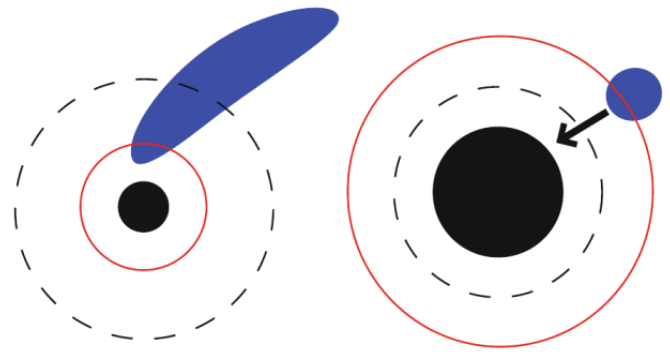
\includegraphics[scale=0.45]{nsbh}
                        \centering
                        \caption{Schematic pictures for the outcome of the merger process, depending on the relative position of $d_{tid}$ and $R_{ISCO}$. The solid filled circle denotes the BH, the distorted ellipsoid denotes the NS, the solid circle is the location of $R_{ISCO}$, and the dashed circle is the location of  $d_{tid}$. Left: the NS is tidally disrupted, and the spatial extent of the disrupted material is larger than or as large as that of the BH. Right: the NS is not tidally disrupted.}
                         \label{fig:nsbh}
                \end{figure}
        As the binary spirals in, the transition to a dynamically plunging orbit happens
        when the NS first reaches either the innermost stable circular orbit $R_{ISCO}$ of the BH, or the tidal disruption distance $d_{tid}$,
        the distance at which the BH gravitational field is able to induce the tidal disruption of the star.
        Depending on the relative position of $R_{ISCO}$ and the $d_{tid}$ there are
        two possible classes of events, as seen in Fig.$\ref{fig:nsbh}$, with very distinct observational properties;
        however, the final remnant of a NSBH merger is always a BH.
        Both the GW emission features and the possibility that NSBH binaries have an EM counterpart
        depends crucially on whether or not the NS is tidally disrupted. \\
        If $d_{tid} \geq R_{ISCO}$ the NS will be tidally disrupted by the tidal field of the BH
        and some debris are left outside the BH after merger.
        When this matter is present outside the BH, EM emission is expected to emerge from a variety of processes.
        Otherwise, if $d_{tid} \leq R_{ISCO}$ the NS plunges into the BH whole and no matter is left outside,
        and very low chances of detectable post-merger EM signals.
        The GW signal is practically identical to a BBH system with the same component masses and spins [35, 70]. \\
        In the merger phase and remnant-formation phase, the dynamics of the system depends
	strongly on the BH and NS mass ratio $q$ defined as $M_{BH}/M_{NS} > 1$, and on the BH spin $\chi_{BH}$.
        The NS tidal deformability $\lambda_{NS}$ also plays a key role in the evolution of the binary:
        the two-body attractive force is strengthen by the effect of the tidal deformation and, by this,
        the orbital separation of the $R_{ISCO}$ is increased and the GW  signal  is  cut  off  when
        disruption occurs. \\
        The main observable effect of the finite size of NS before merger is the acceleration of the GW-driven inspiral
        because the orbital velocity and the centrifugal force has to be increased to maintain circular orbits
        in an enhanced attractive force: large NS merge earlier than more compact stars.
        For a fixed BH mass, a more massive NS requires a larger BH spin in order to be tidally disrupted.
        Indeed high-mass NS are generally more compact, thus $d_{tid}$ is smaller and also
        $R_{ISCO}$ must be small for the BH gravity gradient to unbind material.
        This translates into a larger required BH spin. For a fixed NS mass, more massive BHs have larger
        $R_{ISCO}$, unless their spin is very high. Thus also in this case a high BH spin is required
        to  avoid  a  direct  plunge.  Therefore,  the  best  combination  of binary parameters,
        necessary to induce the NS tidal disruption and release neutron-rich matter, requires $q$ and high $\chi_{BH}$
        At fixed BH and NS masses, the release of ejecta depends on the NS EOS or, equivalently,
        on its $\lambda_{NS}$ defined as
                \begin{equation}
                        \lambda_{NS} = {{2} \over {3}} k_2 C_{NS}^{-5}
                \end{equation}
        where $C_{NS} = M_{NS}/R_{NS}$ and $k_2$ is the dimensionless Love number.

\section{Tidal disruption model}

        Tidal disruption occurs when  the  tidal force of the BH at the surface of the NS is stronger
        than the self-gravity of the NS.  Assuming Newtonian gravity, this condition is approximately
                \begin{equation}
                        {{M_{NS}} \over {R_{NS}^2}} \sim {{3M_{BH}} \over {d_{tid}^3}}R_{NS}
                \end{equation}
        from which tidal disruption is simply $d_{tid} \sim (M_{BH}/M_{NS})^{1/3}R_{NS}$.
        A few tens of milliseconds after tidal disruption occurs the remnant consists of
        a remnant BH and tidal debris containing gravitationally bound and unbound matter.
        Some material gravitationally bound to the remnant swerves
        into an approximately axisymmetric disk around the BH, while some debris material,
        a large amount of neutron-rich material, is dynamically ejected and spread outwards at mildly relativistic speeds.
        The accretion disk an spread to larger radii to conserve angular momentum in the rotational period $\sim 10 ms$,
        rather than being confined within the circularizing radius, resulting in a gradual mass infall into the BH over longer timescales, $\sim 0.1-1 s$.
        However, the mass accretion time scale is much longer than the rotational period, and hence, the disk remains quasi-stationary for $\gg 10 ms$.
        With the intention of obtaining accurate predictions for identifying and characterising NSBH mergers
        a model for the remnant mass outside the BH is needed.
        Whether or not this event can result in SGRBs emission,
        Since NSBH systems cover a high-dimensional and largely unconstrained parameter space,
        understanding whether or not these events can result in SGRBs emission requires to
        derive limits on the range of binary parameters leading to the disruption of a NS.
        Originally, Foucart proposed a model to calculate the amount of matter remaining
        outside the BH about $10ms$ after a BHNS merger, $M_{rem}$, based on comparison
        between $d_{tid}$ and $R_{ISCO}$:
                \begin{equation}
                        {{M_{rem}^{model}} \over {M^b_{NS}}} = \alpha(3q)^{1/3}(1 - 2C_{NS}) - \beta{{R_{ISCO}} \over {R_{NS}}}
                \end{equation}
        where $\alpha$ and $\beta$ are the free parameters of the model,
        and $M^b_{NS}$ is the baryon mass of the NS.
        Since applying the $d_{tid}$ derived from Newtonian gravity to compact object results in underestimating the $C_{NS}$,
        a more appropriate estimation of this quantity, in which compact objects are more strongly bound is
                \begin{equation}
                        \hat{d}_{tid} = d_{tid} (1 - 2C_{NS})
                \end{equation}
        This simple model applies to BH spins aligned with the orbital angular momentum and remnants below
        $\sim 20-25\%$ of the NS mass, leaving out unexplored regions of the parameter space,
        such as comparable masses and high spins.
        To better constraint $M_{rem}$, a new model was proposed by Foucart, Hinderer and Nissanke.
                \begin{equation}
                        {{M_{rem}^{model}} \over {M^b_{NS}}} = \Bigg[ Max \Bigg( \alpha{{1 - 2C_{NS}} \over {\eta^{1/3}}} - \beta {{R_{ISCO}C_{NS}} \over{\eta M_{BH}}} + \gamma, 0 \Bigg)\Bigg]^{\delta}
                \end{equation}



\section{Electromagnetic Counterpart of a Black Hole-Neutron Star Binary Merger}


%----------------------------------------------------------------------------------------------------------------------------------------------------------------------------------------------------------
\chapter{My contribution to gravitational dave data analysis during O3}

	GW170817 not only marked the beginning of a new era in multi-messenger astronomy, 
	but was also a major step forward towards the understanding of the puzzling origins of SGRB. 
	Since then more efforts are now being directed toward optimising the search to take full advantage 
	of the potential for joint GRB-GW events observations.
	In a coherent GW search triggered by SGRBs, template banks play a crucial role in finding the data buried in noise, 
	therefore it is extremely important that they are generated under certain conditions.
	The strong dependence of the GW signal on the component masses and spins, 
	as well as the orientation of the source relative to the detectors, 
	requires that the template bank covers the region of this parameter space 
	that is expected to include the progenitors of short GRBs.
	At the same time it should not exceed this region by too much, 
	as this will make the analysis computationally infeasible and increase the number of background triggers. 
	In order to better discriminate NSBH systems that could produce an accretion disk from this disruption,
	Eq. 5.5 has been replaced by Eq. 5.7 in the generation of the template bank.

\section{Bank Tests}

	The new template bank generates a large set of point within the mass and spin parameter space,
	with the desired minimum $M_{rem}$, then it checks if the systems produce an EM counterpart.
	This means they are required to produce a remnant mass disk: 
	if they do EOS data are loaded and the minimum $\eta$ needed to generate a given $M_{rem}$,
	as a function of $M_{NS}$ and $\chi_{BH}$,  is computed;
	if this is not the case the binary is treated as point particle binaries.
	All system that produce the given $M_{rem}$ make the cut and are stored: 
	as the EM cut can remove several randomly generated binaries, 
	the numbers of accepted points needs to be tracked and stopped when they are enough.
	First all EM dark systems needs to be identified using the logical mask ‘\textbf{{\color{red}mask\_not\_bbh}}, 
	which track points that are not BBH: a point is kept if the secondary object is not a BH, 
	then its masses and spins are stored.
	After this first cut only BNS and NSBH systems are left. 
	To discriminate between these two classes, another requirement is that the secondary mass is a NS, 
	so that ‘\textbf{{\color{green}mask\_bns}}’ identifies only BNS, while the systems that do not satisfy this conditions 
	are identified by ‘\textbf{{\color{black}masknsbh}}’.	
	All these point’s masses and spin are stored.
	As previously showed in Chapter 5, not all NSBH coalescence produce an EM counterpart, 
	so the next step is to cut all systems whose $M_{rem}$ is lower that the threshold mass, 
	identify these points with ‘\textbf{{\color{blue}mask\_nsbh\_bright}}’ and store their masses and spins. 

\begin{table}[]
\begin{tabular}{|l|l|l|l|l|} \hline
\textbf{BNS}  & \textbf{NSBH}       & \textbf{NSBH}    & \textbf{BBH}     \\
EM-bright     & EM-bright  & EM-dim  & EM-dim  \\\hline
{\color{red}1}0{\color{green}1}  & {\color{red}1}1{\color{green}0}{\color{blue}1}  & {\color{red}1}1{\color{green}0}{\color{blue}0}  & {\color{red}0}  \\ \hline
\end{tabular}
\end{table}

\section{O3 offline pyGRB analysis}

\subsection{GRB190425089}

\subsection{GRB190627A}

\subsection{GRB190728271}

\section{PyCBC O3 HL C00 data preliminary runs}

\subsection{Chunk 29}

%--------------------------------------------------------
\chapter{Conclusions}

\backmatter
\cleardoublepage

\phantomsection % Give this command only if hyperref is loaded \addcontentsline{toc}{chapter}{\bibname}

\begin{thebibliography}{500}

	\bibitem{1} Albert Einstein. On the General Theory of Relativity. Sitzungsber. Preuss. Akad. Wiss. Berlin (Math. Phys.), 1915:778–786, 1915. [Addendum: Sitzungsber. Preuss. Akad. Wiss. Berlin (Math. Phys.)1915,799(1915)]. 
	\bibitem{2} Albert Einstein. Naherungsweise integration der feldgleichungen der gravitation. Sitzungsberichte der Koniglich Preu{\ss}ischen Akademie der Wissenschaften (Berlin), 1:688–696, 1916. 
	\bibitem{3} M. Maggiore. Gravitational Waves: Volume 1: Theory and Experiments. Oxford University Press, 2008
	\bibitem{4} E. E. Flanagan and S.A .Hughes. The basics of gravitational wave theory. arXiv:gr-qc/0501041v3
	\bibitem{5} M. Blau, “Lecture Notes on General Relativity,” ICTP (2000). 
	\bibitem{6} Tjonnie G. F. Li. A. Extracting Physics from Gravitational Waves: Testing the Strong-field Dynamics of General Relativity and Inferring the Large-scale Structure of the Universe. Springer, 3 lug 2015	
	\bibitem{7} J. Weber. Detection and generation of gravitational waves. Phys. Rev., 117: 306–313, Jan 1960. doi:10.1103/PhysRev.117.306. 
	\bibitem{8} Gertsenshtein M.E.; Pustovoit V.I. On the detection of low frequency gravitational waves. Sov. J. Exp. Theor. Phys. 1962, 43, 605–607. 
	\bibitem{9} Yu, Haocun and others. Quantum correlations between the light and kilogram-mass mirrors of LIGO. [arXiv:2002.01519 [quant-ph]].
	\bibitem{10} Weinstein, A. Advanced LIGO optical configuration and prototyping effort. Class. Quantum Grav. 19, 1575–1584 (2002).
	\bibitem{11} D. G. Blair, E. J. Howell, L. Ju, C. Zhao. Advanced Gravitational Wave Detectors. Cambridge University Press, 16 feb 2012 
	\bibitem{12} Stephen Fairhurst. Triangulation of gravitational wave sources with a network of detectors. arXiv:0908.2356v2 [gr-qc]
	\bibitem{13} The LIGO Scientific Collaboration, the Virgo Collaboration. GWTC-1: A Gravitational-Wave Transient Catalog of Compact Binary Mergers Observed by LIGO and Virgo during the First and Second Observing Runs.arXiv:1811.12907v3 [astro-ph.HE]
	\bibitem{14} The LIGO Scientific Collaboration, the Virgo Collaboration. GW150914: First results from the search for binary black hole coalescence with Advanced LIGO. arXiv:1602.03839v3 [gr-qc]
        \bibitem{15} B.P. Abbott et al. (LIGO Scientific Collaboration and Virgo Collaboration). GW170817: Observation of Gravitational Waves from a Binary Neutron Star Inspiral. Phys. Rev. Lett. 119, 161101.	
	\bibitem{16} Charles W. Misner, Kip S. Thorne, and John Archibald Wheeler. Gravitation. W. H. Freeman, 1973
	\bibitem{17} Sean M. Carroll. Lecture Notes on General Relativity. arXiv:gr-qc/9712019v1
	\bibitem{18} B.S. Sathyaprakash, B.F. Schutz. Physics, Astrophysics and Cosmology with Gravitational Waves. arXiv:0903.0338v1 [gr-qc]
	\bibitem{19} Schutz, B. F. and Tinto, M. Antenna patterns of interferometric detectors of gravitational waves. I - Linearly polarized (ISSN 0035-8711), vol. 224, Jan. 1, 1987, p. 131-154.
	\bibitem{20} Francesco Zappa, Sebastiano Bernuzzi, Francesco Pannarale, Michela Mapelli, and Nicola Giacobbo. Black-Hole Remnants from Black-Hole–Neutron-Star Mergers. Phys. Rev. Lett. 123, 041102. 
	\bibitem{21} The LIGO Scientific Collaboration, the Virgo Collaboration. The basic physics of the binary black hole merger GW150914. arXiv:1608.01940v4 [gr-qc].
	\bibitem{22} C. J. Moore, R. H. Cole and C. P. L. Berry. Gravitational-wave sensitivity curves. Classical and Quantum Gravity, Volume 32, Number 1
	\bibitem{23} The LIGO Scientific Collaboration and the Virgo Collaboration. Tests of General Relativity with the Binary Black Hole Signals from the LIGO-Virgo Catalog GWTC-1. arXiv:1903.04467v3 [gr-qc].
	\bibitem{24} Bruce Allen. A chi-squared time–frequency discriminator for gravitational wave detection. Phys. Rev. D 71, 062001 (2005).
  	\bibitem{25} Collin Capano, Ian Harry, Stephen Privitera, and Alessandra Buonanno. Implementing a search for gravitational waves from non-precessing, spinning binary black holes. arXiv:1602.03509.
  	\bibitem{26} L. Wen et al 2008. Geometrical expression of the angular resolution of a network of gravitational-wave detectors and improved localization methods. J. Phys.: Conf. Ser. 122 012038.
	\bibitem{27} I. Harry, J. Calderon Bustillo, and A. Nitz, (2017). Searching for the full symphony of black hole binary mergers. arXiv:1709.09181 [gr-qc]. 
  	\bibitem{28} Samantha A. Usman et al. The PyCBC search for gravitational waves from compact binary coalescence.  Classical Quantum Gravity 33, 215004 (2016). 
  	\bibitem{29} Javier Roulet, Liang Dai, Tejaswi Venumadhav, Barak Zackay, and Matias Zaldarriaga. Template bank for compact binary coalescence searches in gravitational wave data: A general geometric placement algorithm. Phys. Rev. D 99, 123022. 
	\bibitem{30} S. Babak, R. Balasubramanian, D. Churches, T. Cokelaer, and B. S. Sathyaprakash. A template bank to search for gravitational waves from inspiralling compact binaries. I: Physical models. Class. Quant. Grav., 23:5477–5504, 2006. 
	\bibitem{31} Benjamin J. Owen, B. S. Sathyaprakash. Matched filtering of gravitational waves from inspiraling compact binaries: Computational cost and template placement. arXiv:gr-qc/9808076v1
	\bibitem{32} P. Ajith, N. Fotopoulos, S. Privitera, A. Neunzert, N. Mazumder, A. J. Weinstein. An effectual template bank for the detection of gravitational waves from inspiralling compact binaries with generic spins. arXiv:1210.6666v2.
	\bibitem{33} B. J. Owen. Search templates for gravitational waves from inspiraling binaries: Choice of template spacing. Phys. Rev. D 53, 6749 (1996). 
	\bibitem{34} I. W. Harry, B. Allen, and B. S. Sathyaprakash. A stochastic template placement algorithm for gravitational wave data analysis. Phys. Rev. D 80, 104014 (2009).  
	\bibitem{35} S. Roy, A. S. Sengupta, and N. Thakor. A hybrid geometric-random template placement algorithm for gravitational wave searches from compact binary coalescences. Phys. Rev. D 95, 104045 (2017). 
	\bibitem{36} N. Indik, K. Haris, T. Dal Canton, H. Fehrmann, B. Kr- ishnan, A. Lundgren, A. B. Nielsen, and A. Pai. A stochastic template bank for gravitational wave searches for precessing neutron-star--black-hole coalescence events. Phys. Rev. D95, 064056 (2017), arXiv:1612.05173 [gr-qc].  
	\bibitem{37} Maccarone, T., and Knigge, C. Compact objects in globular clusters. Astron. Geophys. 48 5.12- 5.20 (2007)
	\bibitem{38} Harry I, Privitera S, Bohé A, Buonanno A (2016) Searching for gravitational waves from compact binaries with precessing spins. Phys Rev D 94:024012. https://doi.org/10.1103/PhysRevD.94.024012. arXiv:1603.02444
	\bibitem{39} Katerina Chatziioannou, Antoine Klein, Nicolás Yunes, and Neil Cornish. Constructing gravitational waves from generic spin-precessing compact binary inspirals. Phys. Rev. D 95, 104004
	\bibitem{40} L. K. Nuttall, T. J. Massinger, J. Areeda, J. Betzwieser, S. Dwyer, A. Effler, R. P. Fisher, P. Fritschel, J. S. Kissel, A. P. Lundgren, D. M. Macleod, D. Martynov, J. McIver, A. Mullavey, D. Sigg, J. R. Smith, G. Vajente, A. R. Williamson, C. C. Wipf. Improving the data quality of Advanced LIGO based on early engineering run results. arXiv:1508.07316v2 [gr-qc].
	\bibitem{41} Alexander H Nitz. Distinguishing short duration noise transients in LIGO data to improve the PyCBC search for gravitational waves from high mass binary black hole mergers. arXiv:1709.08974v2 [gr-qc].
	\bibitem{42} The LIGO Scientific Collaboration, the Virgo Collaboration. Effects of Data Quality Vetoes on a Search for Compact Binary Coalescences in Advanced LIGO's First Observing Run. arXiv:1710.02185v4 [gr-qc].
	\bibitem{43} Gareth S. Davies, Thomas Dent, Márton Tápai, Ian Harry, Connor McIsaac, Alexander H. Nitz. Extending the PyCBC search for gravitational waves from compact binary mergers to a global network. arXiv:2002.08291v2 [astro-ph.HE].
	\bibitem{44} LIGO Scientific, Virgo Collaboration, B. P. Abbott et al., A guide to LIGO-Virgo detector noise and extraction of transient gravitational-wave signals, Class. Quant. Grav. 37 (2020) 055002, [arXiv:1908.11170]. 
	\bibitem{45} Macleod D., Harry I. W. and Fairhurst S. A fully-coherent all-sky search for gravitational-waves from compact binary coalescences. 2016 Phys. Rev. D93 064004. 
	\bibitem{46} Williamson A., Biwer C., Fairhurst S. et al. Improved methods for detecting gravitational waves associated with short gamma-ray bursts. 2014 PhRvD 90 122004.
	\bibitem{47} S. Babak et al. Searching for gravitational waves from binary coalescence. Phys. Rev. D 87, 024033.
	\bibitem{48} Juan Calderón Bustillo, Francesco Salemi, Tito Dal Canton, and Karan P. Jani.Sensitivity of gravitational wave searches to the full signal of intermediate-mass black hole binaries during the first observing run of Advanced LIGO. Phys. Rev. D 97, 024016.
	\bibitem{49} Carl-Johan Haster, Zhilu Wang, Christopher P. L. Berry, Simon Stevenson, John Veitch, Ilya Mandel. Inference on gravitational waves from coalescences of stellar-mass compact objects and intermediate-mass black holes. https://doi.org/10.1093/mnras/stw233.
	\bibitem{50} C. Biwer et al. Validating gravitational-wave detections: The Advanced LIGO hardware injection system. Phys. Rev. D 95, 062002.
	\bibitem{51} Vassiliki Kalogera and Albert Lazzarini. LIGO and the opening of a unique observational window on the universe. PNAS March 21, 2017 114 (12) 3017-3025.
	\bibitem{52} Abbott, B. P. et al. (LIGO Scientific Collaboration, Virgo Collaboration). Observation of gravitational waves from a binary black hole merger. Phys. Rev. Lett. 116, 061102 (2016).
	\bibitem{53} KAGRA Collaboration, LIGO Scientific Collaboration, and Virgo Collaboration. Prospects for observing and localizing gravitational-wave transients with Advanced LIGO, Advanced Virgo and KAGRA (2019). Preprint at https://arxiv.org/abs/1304.0670. 
         \bibitem{54} Chen, H.-Y. et al. Distance measures in gravitational-wave astrophysics and cosmology (2017). arXiv:1709.08079.
	\bibitem{55} LIGO Scientific Collaboration and Virgo Collaboration et al. 2017b. Gravitational Waves and Gamma-rays from a Binary Neutron Star Merger: GW170817 and GRB 170817A.
	\bibitem{56} Abbott, B. P. et al. (LIGO Scientific Collaboration, Virgo Collaboration). Low-latency Gravitational-wave Alerts for Multimessenger Astronomy during the Second Advanced LIGO and Virgo Observing Run. ApJ 875, 161 (2019). 
	\bibitem{57} Abbott, B. P. et al. (LIGO Scientific Collaboration, Virgo Collaboration). GW150914: First Results from the Search for Binary Black Hole Coalescence with Advanced LIGO. Phys. Rev. D 93, 122003 (2016). 
	\bibitem{58} Abbott, B. P. et al. (LIGO Scientific Collaboration, Virgo Collaboration). GW151226: Observation of Gravitational Waves from a 22-Solar-Mass Binary Black Hole Coalescence. Phys. Rev. Lett. 116, 241103 (2016). 
	\bibitem{59} Abbott, B. P. et al. (LIGO Scientific Collaboration, Virgo Collaboration). Binary Black Hole Mergers in the First Advanced LIGO Observing Run. Phys. Rev. X 6, 041015 (2016).
	\bibitem{60} Abbott, B. P. et al. (LIGO Scientific Collaboration, Virgo Collaboration). GW170104: Observation of a 50-Solar-Mass Binary Black Hole Coalescence at Redshift 0.2. Phys. Rev. Lett. 118, 221101 (2017).
	\bibitem{61} Abbott, B. P. et al. (LIGO Scientific Collaboration, Virgo Collaboration). GW170814: A Three-Detector Observation of Gravitational Waves from a Binary Black Hole Coalescence. Phys. Rev. Lett. 119, 141101 (2017).
	\bibitem{62} Abbott, B. P. et al. (LIGO Scientific Collaboration, Virgo Collaboration). GW170817: Observation of Gravitational Waves from a Binary Neutron Star Inspiral. Phys. Rev. Lett. 119, 161101 (2017).         
	\bibitem{63} Abbott, B. P. et al. Multi-messenger observations of a binary neutron star merger. ApJ 848, L12 (2017).
	\bibitem{64} K. Belczynski, D. E. Holz, T. Bulik, and R. O’Shaugh- nessy, The First Gravitational-Wave Source from the Isolated Evolution of Two 40-100 Msun Stars, Nature (London) 534, 512 (2016)
	\bibitem{65} J. J. Eldridge and E. R. Stanway, BPASS Predictions for Binary Black-Hole Mergers, Mon. Not. R. Astron. Soc. 462, 3302 (2016).
	\bibitem{66} V. M. Lipunov, V. Kornilov, E. Gorbovskoy, N. Tiurina, P. Balanutsa, and A. Kuznetsov, The First Gravitational- Wave Burst GW150914. Part I. Scenario Machine Prediction, New Astron. 51, 122 (2016).
	\bibitem{67} S.E. de Mink and I. Mandel, The Chemically Homogeneous Evolutionary Channel for Binary Black Hole Mergers: Rates and Properties of Gravitational-Wave Events Detectable by Advanced LIGO, Mon. Not. R. Astron. Soc. 460, 3545 (2016).
 	\bibitem{68} K. Inayoshi, K. Kashiyama, E. Visbal, and Z. Haiman, Strong Gravitational Wave Background from Population III Binary Black Holes Consistent with Cosmic Reionization, Mon. Not. R. Astron. Soc. 461, 2722 (2016).
 	\bibitem{69} C. L. Rodriguez, C. J. Haster, S. Chatterjee, V. Kalogera, and F. A. Rasio, Dynamical Formation of the GW150914 Binary Black Hole, Astrophys. J. Lett. 824, L8 (2016). M. Mapelli, Massive Black Hole Binaries from Runaway Collisions: The Impact of Metallicity, Mon. Not. R. Astron. Soc. 459, 3432 (2016).
        \bibitem{70} I. Bartos, B. Kocsis, Z. Haiman, and S. Márka, Rapid and Bright Stellar-Mass Binary Black Hole Mergers in Active Galactic Nuclei, arXiv:1602.03831.
 	\bibitem{71} N. C. Stone, B. D. Metzger, and Z. Haiman, Assisted Inspirals of Stellar Mass Black Holes Embedded in AGN Disks, Mon. Not. R. Astron. Soc., doi: 10.1093/ mnras/stw2260 (2015).
       \bibitem{72} I. Mandel and S. E. de Mink, Merging Binary Black Holes Formed through Chemically Homogeneous Evolution in Short-Period Stellar Binaries, Mon. Not. R. Astron. Soc. 458, 2634 (2016).
         \bibitem{73} P. Marchant, N. Langer, P. Podsiadlowski, T. M. Tauris, and T. J. Moriya, A New Route Towards Merging Massive Black Holes, Astron. Astrophys. 588, A50 (2016).
     \bibitem{74}K. Belczynski, T. Bulik, and B. Rudak, The First Stellar Binary Black Holes: The Strongest Gravitational Wave Burst Sources, Astrophys. J. Lett. 608, L45 (2004).
       \bibitem{75} T. Kinugawa, K. Inayoshi, K. Hotokezaka, D. Nakauchi, and T. Nakamura, Possible Indirect Confirmation of the Existence of Pop III Massive Stars by Gravitational Wave, Mon. Not. R. Astron. Soc. 442, 2963 (2014).
         \bibitem{76} A. Tutukov and L. Yungelson, Evolution of Massive Close Binaries, Nauchnye Informatsii 27, 70 (1973).
         \bibitem{77} A. V. Tutukov and L. R. Yungelson, The Merger Rate of Neutron Star and Black Hole Binaries, Mon. Not. R. Astron. Soc. 260, 675 (1993).
        \bibitem{78} V. M. Lipunov, K. A. Postnov, and M. E. Prokhorov, Formation and Coalescence of Relativistic Binary Stars: The Effect of Kick Velocity, Mon. Not. R. Astron. Soc. 288, 245 (1997).
        \bibitem{79} R. Voss and T. M. Tauris, Galactic Distribution of Merging Neutron Stars and Black Holes—Prospects for Short Gamma-Ray Burst Progenitors and LIGO/Virgo, Mon. Not. R. Astron. Soc. 342, 1169 (2003).
        \bibitem{80} G. Nelemans, Galactic Binaries as Sources of Gravitational Waves, in Astrophysics of Gravitational Wave Sources, American Institute of Physics Conference Series, edited by J.M. Centrella (AIP, Melville, NY, 2003), Vol. 686, pp. 263–272.
         \bibitem{81} K. Belczynski, M. Dominik, T. Bulik, R. O’Shaughnessy, C. Fryer, and D. E. Holz, The Effect of Metallicity on the Detection Prospects for Gravitational Waves, Astrophys. J. Lett. 715, L138 (2010).
         \bibitem{82} B. McKernan, K. E. S. Ford, W. Lyra, and H. B. Perets, Intermediate Mass Black Holes in AGN DiscsI. Production and Growth, Mon. Not. R. Astron. Soc. 425, 460 (2012).
         \bibitem{83} J.M. Bellovary, M.-M. Mac Low, B. McKernan, and K. E. S. Ford, Migration Traps in Disks around Super- massive Black Holes, Astrophys. J. Lett. 819, L17 (2016).
         \bibitem{84} S. Sigurdsson and L. Hernquist, Primordial Black Holes in Globular Clusters, Nature (London) 364, 423 (1993).
        \bibitem{85} S. F. Portegies Zwart and S. L. W. McMillan, Black Hole Mergers in the Universe, Astrophys. J. 528, L17 (2000).
        \bibitem{86} M. C. Miller and V. M. Lauburg, Mergers of Stellar-Mass Black Holes in Nuclear Star Clusters, Astrophys. J. 692, 917 (2009).
        \bibitem{87} B. M. Ziosi, M. Mapelli, M. Branchesi, and G. Tormen, Dynamics of Stellar Black Holes in Young Star Clusters with Different Metallicities II. Black Hole-Black Hole Binaries, Mon. Not. R. Astron. Soc. 441, 3703 (2014).
         \bibitem{88} C.L. Rodriguez, M. Morscher, B. Pattabiraman, S. Chatterjee, C.-J. Haster, and F.A. Rasio, Binary Black Hole Mergers from Globular Clusters: Implications for Advanced LIGO, Phys. Rev. Lett. 115, 051101 (2015).
         \bibitem{89} C. P. L. Berry et al., Parameter Estimation for Binary Neutron-Star Coalescences with Realistic Noise During the Advanced LIGO Era, Astrophys. J. 804, 114 (2015).
 	\bibitem{90} S. Fairhurst, Source Localization with an Advanced Gravitational Wave Detector Network, Classical Quantum Gravity 28, 105021 (2011).
         \bibitem{91} L. P. Singer and L. R. Price, Rapid Bayesian Position Reconstruction for Gravitational-Wave Transients, Phys. Rev. D 93, 024013 (2016).
   	\bibitem{92} S. Fairhurst, Triangulation of Gravitational Wave Sources with a Network of Detectors, New J. Phys. 11, 123006 (2009).
    	\bibitem{93} B. P. Abbott, R. Abbott, T. D. Abbott et al. (LIGO Scientific Collaboration and Virgo Collaboration), Properties of the Binary Black Hole Merger GW150914, Phys. Rev. Lett. 116, 241102 (2016).
 	\bibitem{94} S. Vitale, R. Lynch, J. Veitch, V. Raymond, and R. Sturani, Measuring the Spin of Black Holes in Binary Systems Using Gravitational Waves, Phys. Rev. Lett. 112, 251101 (2014). 
 	\bibitem{95} M. V. van der Sluys, C. Roever, A. Stroeer, N. Christensen, V. Kalogera, R. Meyer, and A. Vecchio, Gravitational- Wave Astronomy with Inspiral Signals of Spinning Compact-Object Binaries,        Astrophys. J. 688, L61 (2008).
         \bibitem{96}S. Nissanke, D. E. Holz, S. A. Hughes, N. Dalal, and J. L. Sievers, Exploring Short Gamma-Ray Bursts as Gravitational-Wave Standard Sirens, Astrophys. J. 725, 496 (2010).
         \bibitem{97} B. Farr et al., Parameter Estimation on Gravitational Waves from Neutron-Star Binaries with Spinning Components, Astrophys. J. 825, 116 (2015).
    	\bibitem{98} C. Cutler and E. Flanagan, Gravitational Waves from Merging Compact Binaries: How Accurately Can One Extract the Binary’s Parameters from the Inspiral Waveform?, Phys. Rev. D 49, 2658 (1994) 
   	\bibitem{99} J. A. Gonzalez, U. Sperhake, B. Brügmann, M. Hannam, and S. Husa, Total Recoil: The Maximum Kick from Nonspinning Black-Hole Binary Inspiral, Phys. Rev. Lett. 98, 091101 (2007).
        \bibitem{100} E. Berti, V. Cardoso, J.A. Gonzalez, U. Sperhake, M. Hannam, S. Husa, and B. Brügmann, Inspiral, Merger and Ringdown of Unequal Mass Black Hole Binaries: A Multipolar Analysis, Phys. Rev. D 76, 064034 (2007).
         \bibitem{101} J. G. Baker, W. D. Boggs, J. Centrella, B. J. Kelly, S. T. McWilliams, and J.R. van Meter, Mergers of Non- spinning Black-Hole Binaries: Gravitational Radiation Characteristics, Phys. Rev. D 78, 044046 (2008). 
        \bibitem{102} C. Reisswig, S. Husa, L. Rezzolla, E.N. Dorband, D. Pollney, and J. Seiler, Gravitational-Wave Detectability of Equal-Mass Black-Hole Binaries with Aligned Spins, Phys. Rev. D 80, 124026 (2009). 
    	\bibitem{103} A. Taracchini, A. Buonanno, Y. Pan, T. Hinderer, M. Boyle et al., Effective-One-Body Model for Black-Hole Binaries with Generic Mass Ratios and Spins, Phys. Rev. D 89, 061502 (2014).
         \bibitem{104} M. Pürrer, Frequency Domain Reduced Order Model of Aligned-Spin Effective-One-Body Waveforms with Generic Mass-Ratios and Spins, Phys. Rev. D 93, 064041 (2016). 
        \bibitem{105} S. Husa, S. Khan, M. Hannam, M. Pürrer, F. Ohme, X. J. Forteza, and A. Bohé, Frequency-Domain Gravitational Waves from Nonprecessing Black-Hole Binaries. I. New Numerical Waveforms and Anatomy of the Signal, Phys. Rev. D 93, 044006 (2016).
         \bibitem{106}  S. Khan, S. Husa, M. Hannam, F. Ohme, M. Prrer, X. J. Forteza, and A. Boh, Frequency-Domain Gravitational Waves from Non-precessing Black-Hole Binaries. II. A Phenomenological Model for the Advanced Detector Era, Phys. Rev. D 93, 044007 (2016).
         \bibitem{107} M. Hannam, P. Schmidt, A. Bohé, L. Haegel, S. Husa, F. Ohme, G. Pratten, and M. Pürrer, Simple Model of Complete Precessing Black-Hole-Binary Gravitational Waveforms, Phys. Rev. Lett. 113, 151101 (2014).
         \bibitem{108} B. P. Abbott, R. Abbott, T. D. Abbott et al. (LIGO Scientific Collaboration and Virgo Collaboration), GW150914: The Advanced LIGO Detectors in the Era of First Discoveries, Phys. Rev. Lett. 116, 131103 (2016).
         \bibitem{109} T. Dal Canton et al., Implementing a Search for Aligned- Spin Neutron Star-Black Hole Systems with Advanced Ground Based Gravitational Wave Detectors, Phys. Rev. D 90, 082004 (2014).
 	\bibitem{110} S. A. Usman et al., An Improved Pipeline to Search for Gravitational Waves from Compact Binary Coalescence, arXiv:1508.02357.
        \bibitem{111} A. H. Nitz, I. W. Harry, J. L. Willis, C. M. Biwer, D. A. Brown, L. P. Pekowsky, T. Dal Canton, A. R. Williamson, T. Dent, C. D. Capano et al., PyCBC Software, https:// github.com/ligo!cbc/pycbc.
        \bibitem{112} K. Cannon, R. Cariou, A. Chapman, M. Crispin-Ortuzar, N. Fotopoulos et al., Toward Early-Warning Detection of Gravitational Waves from Compact Binary Coalescence, Astrophys. J. 748, 136 (2012).
 	\bibitem{113} S. Privitera, S. R. P. Mohapatra, P. Ajith, K. Cannon, N. Fotopoulos, M.A. Frei, C. Hanna, A.J. Weinstein, and J. T. Whelan, Improving the Sensitivity of a Search for Coalescing Binary Black Holes with Nonprecessing Spins in Gravitational Wave Data, Phys. Rev. D 89, 024003 (2014).
         \bibitem{114} C. Messick, K. Blackburn, P. Brady, P. Brockill, K. Cannon, S. Caudill, S. J. Chamberlin, J. D. E. Creighton, R. Everett, C. Hanna et al., Analysis Framework for the Prompt Discovery of Compact Binary Mergers in Gravi- tational-wave Data, arXiv:1604.04324
         \bibitem{115} A. Effler, R. M. S. Schofield, V. V. Frolov, G. Gonzalez, K. Kawabe, J. R. Smith, J. Birch, and R. McCarthy, Envi- ronmental Influences on the LIGO Gravitational Wave Detectors During the 6th Science Run, Classical Quantum Gravity 32, 035017 (2015). 
        \bibitem{116} B.P. Abbott et al. (LIGO Scientific Collaboration and Virgo Collaboration), Effects of Data Quality Vetoes on a Search for Compact Binary Coalescences in Ad- vanced LIGO’s First Observing Run 
        \bibitem{117} L. A. Wainstein and V. D. Zubakov, Extraction of Signals from Noise (Prentice-Hall, Englewood Cliffs, NJ, 1962). 
         \bibitem{118} K. S. Thorne, Gravitational Radiation, in Three Hundred Years of Gravitation, edited by S. W. Hawking and W. Israel (Cambridge University Press, Cambridge, England, 1987), Chap. 9, pp. 330–458. 
        \bibitem{119} B. S. Sathyaprakash and S. V. Dhurandhar, Choice of Filters for the Detection of Gravitational Waves from Coalescing Binaries, Phys. Rev. D 44, 3819 (1991). 
 	\bibitem{120} C. Cutler et al., The Last Three Minutes: Issues in Gravitational Wave Measurements of Coalescing Compact Binaries, Phys. Rev. Lett. 70, 2984 (1993).
 	\bibitem{121} C. E. Rhoades, Jr. and R. Ruffini, Maximum Mass of a Neutron Star, Phys. Rev. Lett. 32, 324 (1974). 
	\bibitem{122} V. Kalogera and G. Baym, The Maximum Mass of a Neutron Star, Astrophys. J. 470, L61 (1996). 
	\bibitem{123} F. Ozel, D. Psaltis, R. Narayan, and J. E. McClintock, The Black Hole Mass Distribution in the Galaxy, Astrophys. J. 725, 1918 (2010). 
	\bibitem{124} W. M. Farr, N. Sravan, A. Cantrell, L. Kreidberg, C. D. Bailyn, I. Mandel, and V. Kalogera, The Mass Distribution of Stellar-Mass Black Holes, Astrophys. J. 741, 103 (2011). 
	\bibitem{125} L. Kreidberg, C. D. Bailyn, W. M. Farr, and V. Kalogera, Mass Measurements of Black Holes in X-Ray Transients: Is There a Mass Gap?, Astrophys. J. 757, 36 (2012). 
	\bibitem{126} L. Blanchet, T. Damour, B. R. Iyer, C. M. Will, and A. G. Wiseman, Phys. Rev. Lett. 74, 3515 (1995).
	\bibitem{127} C. Cutler and E. E. Flanagan, Phys. Rev. D 49, 2658 (1994). 
	\bibitem{128} F. Ohme, A.B. Nielsen, D. Keppel, and A. Lundgren, Statistical and Systematic Errors for Gravitational-Wave Inspiral Signals: A Principal Component Analysis, Phys. Rev. D 88, 042002 (2013). 
	\bibitem{129} J. Antoniadis, P. C. C. Freire, N. Wex, T. M. Tauris, R. S. Lynch et al., A Massive Pulsar in a Compact Relativistic Binary, Science 340, 1233232 (2013). 
	\bibitem{130} K. Belczynski, A. Buonanno, M. Cantiello, C. L. Fryer, D. E. Holz, I. Mandel, M. C. Miller, and M. Walczak, The Formation and Gravitational-Wave Detection of Massive Stellar Black-Hole Binaries, Astrophys. J. 789, 120 (2014). 
	\bibitem{131} We quote the matched-filter SNR as computed by the PyCBC search using the updated calibration; the GstLAL values agree within 2\%. 
	\bibitem{132} C. E. Rhoades, Jr. and R. Ruffini, Maximum Mass of a Neutron Star, Phys. Rev. Lett. 32, 324 (1974).
        \bibitem{132} The LIGO Scientific Collaboration, the Virgo Collaboration. GW190412: Observation of a Binary-Black-Hole Coalescence with Asymmetric Masses. arXiv:2004.08342.
	\bibitem{134} B. P. Abbott et al. (LIGO Scientific Collaboration, Virgo Collaboration), Astrophysical Implications of the Binary Black-Hole Merger GW150914. Astrophys. J. Lett. 818, L22 (2016), arXiv:1602.03846 [astro-ph.HE]. 
	\bibitem{135} J. S. Vink, New Astron. Rev. 52, 419 (2008).
	\bibitem{136} B. P. Abbott et al. (LIGO Scientific Collaboration, Virgo Collaboration), Phys. Rev. X 6, 041015 (2016), arXiv:1606.04856 [gr-qc]. 
	\bibitem{137} B. P. Abbott et al. (LIGO Scientific Collaboration, Virgo Collaboration), Astrophys. J. Lett. 833, L1 (2016), arXiv:1602.03842 [astro-ph.HE]. 
	\bibitem{138} Cannon et al. 2015; Messick et al. 2017; Adams et al. 2016; Nitz et al. 2017b.
	\bibitem{139} Racine 2008; Ajith et al. 2011.
	\bibitem{140} Abbott et al. 2016e.
	\bibitem{141} Lattimer and Prakash 2016.
	\bibitem{142} Spera et al. 2015.
	\bibitem{143} K. Cannon et al., Astrophys. J. 748, 136 (2012).
	\bibitem{144} C. Messick et al., Phys. Rev. D 95, 042001 (2017).
	\bibitem{145} A. H. Nitz et al., PYCBC Software (GitHub, 2017) [https:// github.com/ligo-cbc/pycbc].
	\bibitem{146} A. H. Nitz, T. Dent, T. Dal Canton, S. Fairhurst, and D. A. Brown, arXiv:1705.01513.
	\bibitem{147} A. H. Nitz, arXiv:1709.08974.
	\bibitem{148} S. A. Usman et al., Classical Quantum Gravity 33, 215004 (2016).
	\bibitem{149} T. Dal Canton et al., Phys. Rev. D 90, 082004 (2014). 
	\bibitem{150} B. Allen, W. G. Anderson, P. R. Brady, D. A. Brown, and J. D. E. Creighton, Phys. Rev. D 85, 122006 (2012).
	\bibitem{151} S. Klimenko et al., Phys. Rev. D 93, 042004 (2016).
	\bibitem{152} J. Veitch et al., Phys. Rev. D 91, 042003 (2015).
	\bibitem{153} Meszaros, P. and Rees, M. J. Relativistic fireballs and their impact on external matter - Models for cosmological gamma-ray bursts. Astrophysical Journal, Part 1 (ISSN 0004-637X), vol. 405, no. 1, p. 278-284. 
	\bibitem{154} L. Blanchet, Living Rev. Relativity 17, 2 (2014).
	\bibitem{155} A. Buonanno and T. Damour, Phys. Rev. D 59, 084006 (1999).
	\bibitem{156} A. Buonanno and T. Damour, Phys. Rev. D 62, 064015 (2000).
	\bibitem{157} T. Damour, P. Jaranowski, and G. Schaefer, Phys. Rev. D 78, 024009 (2008).
	\bibitem{158} T. Damour and A. Nagar, Phys. Rev. D 79, 081503 (2009).
	\bibitem{159} A. Taracchini, A. Buonanno, Y. Pan, T. Hinderer, M. Boyle et al., Phys. Rev. D 89, 061502 (2014).
	\bibitem{160} M. Pürrer, Phys. Rev. D 93, 064041 (2016).
	\bibitem{161} S. Husa, S. Khan, M. Hannam, M. Pürrer, F. Ohme, X. J. Forteza, and A. Bohé, Phys. Rev. D 93, 044006 (2016). 
	\bibitem{162} Metzger, M et al. Spectral constraints on the redshift of the optical counterpart to the gamma-ray burst. 1997, Nature, 387, 878.
	\bibitem{163} M. Hannam, P. Schmidt, A. Bohé, L. Haegel, S. Husa, F. Ohme, G. Pratten, and M. Pürrer, Phys. Rev. Lett. 113, 151101 (2014).
	\bibitem{164} R. Smith, S.E. Field, K. Blackburn, C.-J. Haster, M. Pürrer, V. Raymond, and P. Schmidt, Phys. Rev. D 94, 044031 (2016).
	\bibitem{165} M. M. Kasliwal and S. Nissanke, Astrophys. J. 789, L5 (2014). 
	\bibitem{166} L. P. Singer, L. R. Price, B. Farr, A. L. Urban, C. Pankow et al., Astrophys. J. 795, 105 (2014). 
	\bibitem{167} C. P. L. Berry et al., Astrophys. J. 804, 114 (2015). 
	\bibitem{168} S. Fairhurst, New J. Phys. 11, 123006 (2009); 13, 069602 (E) (2011). 
 	\bibitem{169} S. Fairhurst, Classical Quantum Gravity 28, 105021 (2011). 
 	\bibitem{170} P. Ajith and S. Bose, Phys. Rev. D 79, 084032 (2009). 
 	\bibitem{171} D. M. Eardley, D. L. Lee, A. P. Lightman, R. V. Wagoner, and C. M. Will, Phys. Rev. Lett. 30, 884 (1973). 
 	\bibitem{172} D. M. Eardley, D. L. Lee, and A. P. Lightman, Phys. Rev. D 
 	\bibitem{173} J. M. Weisberg, D. J. Nice, and J. H. Taylor, Astrophys. J. 722, 1030 (2010).
 	\bibitem{174} P. C. C. Freire, N. Wex, G. Esposito-Farese, J. P. W. Verbiest, M. Bailes, B. A. Jacoby, M. Kramer, I. H. Stairs, J. Antoniadis, and G. H. Janssen, Mon. Not. R. Astron. Soc. 423, 3328 (2012).
 	\bibitem{175} I. H. Stairs, Living Rev. Relativity 6, 5 (2003).
 	\bibitem{176} N. Wex, arXiv:1402.5594.
	\bibitem{177} K. S. Thorne, Rev. Mod. Phys. 52, 299 (1980).
        \bibitem{178} A. Einstein, Sitzungsber. Preuss. Akad. Wiss. Berlin (Math. Phys. ) 1918, 154 (1918).
        \bibitem{179} E. T. Newman and R. Penrose, Journal of Mathematical Physics 7, 863 (1966).
	\bibitem{180} Klebesadel et al., 1973. Observations of Gamma-Ray Bursts of Cosmic Origin.
	\bibitem{181} Rees and Meszaros, 1992; Begelman et al., 1993.
	\bibitem{182} Gehrels et al. 2009. Gamma-Ray Bursts in the Swift Era. https://doi.org/10.1146/annurev.astro.46.060407.145147.
	\bibitem{183} Sari et al., 1999. Jets in Gamma-Ray Bursts. The Astrophysical Journal, 519:L17-L20, 1999 July 1.
	\bibitem{184} Meegan et al., 1992. Spatial distribution of gamma-ray bursts observed by BATSE. Nature, Volume 355, Issue 6356, pp. 143-145 (1992).
	\bibitem{185} A. M. Hillas, The origin of ultra-high-energy cosmic rays, ARAA 22, 425 (1984).
	\bibitem{186} B. Zhang, The Physics of Gamma-Ray Bursts (Cambridge University Press, 2018).
	\bibitem{187} L. Blanchet, Living Rev. Relativ. 9 (2006). 
	\bibitem{188} L. Blanchet, G. Faye, B. R. Iyer, and S. Sinha, Classical and Quantum Gravity 25, 165003 (2008). 
	\bibitem{189} L. E. Kidder, Phys. Rev. D 77, 044016 (2008). 
	\bibitem{190} J. Healy, P. Laguna, L. Pekowsky, and D. Shoemaker, Phys. Rev. D 88, 024034 (2013). 
	\bibitem{191} L. London, D. Shoemaker, and J. Healy, Phys. Rev. D 90, 124032 (2014). 
	\bibitem{192} C. K. Mishra, A. Kela, K. G. Arun, and G. Faye, Phys. Rev. D 93, 084054 (2016).
	\bibitem{193} N. J. Cornish and T. B. Littenberg. BayesWave: Bayesian Inference for Gravitational Wave Bursts and Instrument Glitches. Classical Quantum Gravity 32, 135012 (2015). 
\end{thebibliography}

\printbibliography
\end{document} 

